\documentclass{tufte-book}

\hypersetup{colorlinks}

\usepackage{xspace}
\newcommand{\PETSCVERSION}{3.6\xspace}
\newcommand{\PETSCMINORVERSION}{3.6.2\xspace}
\newcommand{\PETSCMONTH}{November 2015\xspace}

\newcommand{\CODELOC}{}  % each Chapter redefines this

\let\STUBSONLY\relax  %                                <--- UNCOMMENT TO GENERATE STUB CHAPTERS
\ifx\STUBSONLY\undefined
  \newcommand{\stubinput}[2]{\input{#1}}
\else
  \newcommand{\stubinput}[2]{\vspace{5cm} \centerline{\LARGE Percent completed:  \Huge #2\%.} \vfill}
\fi

\renewcommand{\maketitlepage}[0]{%
  \cleardoublepage%
  {%
  \sffamily%
  \begin{fullwidth}%
  \fontsize{18}{20}\selectfont\par\noindent\textcolor{darkgray}{\allcaps{\thanklessauthor}}%
  \vspace{9pc}%
  \fontsize{32}{40}\selectfont\par\noindent\textcolor{darkgray}{\allcaps{\thanklesstitle}}%
  \vfill%
    \fontsize{18}{40}\selectfont\par\noindent\textcolor{darkgray}{\allcaps{numerical solutions in C using}}%
    \fontsize{18}{40}\selectfont\par\noindent\textcolor{darkgray}{\allcaps{the Portable, Extensible Toolkit for Scientific computation version \PETSCVERSION}}%
  \vfill%
  \fontsize{14}{16}\selectfont\par\noindent\allcaps{\thanklesspublisher}%
  \end{fullwidth}%
  }
  \thispagestyle{empty}%
  \clearpage%
}

\title[PETSc for PDEs]{PETSc \\ for \\ Partial \\ Differential \\ Equations}

\author{Ed Bueler}
\publisher{Maybe Someday a Publisher of This Book}

\date{\today}

\usepackage{booktabs} % for nicely-typeset tabular material
\usepackage{verbatim} % for "comment" environment
%\usepackage{underscore} % causes "Missing \endcsname inserted" error?
\usepackage{graphicx}
\usepackage{amsmath,amssymb,amsthm,bm}
\usepackage{tikz}

\usetikzlibrary{arrows,decorations.markings,decorations.pathreplacing,fadings}

\usepackage{pgfplots}

\usepackage{newfloat,caption}

\usepackage{fancyvrb}
% an alternative which does not seem to have "start string" and
% "stop string" capabilities:
%\usepackage{listings}

\newtheorem*{theorem}{Theorem}
\theoremstyle{definition}
\newtheorem*{example}{Example}
\newtheorem*{examplecont}{Example, continued}

% Prints an epigraph and speaker in sans serif, all-caps type.
\newcommand{\openepigraph}[2]{%
  %\sffamily\fontsize{14}{16}\selectfont
  \begin{fullwidth}
  \sffamily\large
  \begin{doublespace}
  \noindent\allcaps{#1}\\% epigraph
  \noindent \Large \allcaps{#2}% author
  \end{doublespace}
  \end{fullwidth}
}

\newcommand{\monthyear}{%
  \ifcase\month\or January\or February\or March\or April\or May\or June\or
  July\or August\or September\or October\or November\or
  December\fi\space\number\year
}


% the goal here is to have a display of code with a separate "Code x.y" numbering
% and with the caption in the margin
\DeclareFloatingEnvironment[placement={!ht},name=Code]{mycodeenv}
\captionsetup[mycodeenv]{labelfont=bf}
% next line duplicates declaration of environment "marginfigure" in tufte-common.def
\newenvironment{margincode}[1][-1.2ex]%
  {\begin{@tufte@margin@float}[#1]{mycodeenv}}
  {\end{@tufte@margin@float}}

\newcommand{\trueinput}[2]{
\VerbatimInput[frame=single,framesep=3mm,label=\fbox{\normalsize \textsl{\,#1\,}},fontfamily=courier,fontsize=\footnotesize]{#2}
}

%\inputfromline{FULLPATH}{FILENAME}{CAPTION}{FIRSTLINE}{LABEL}
\newcommand{\inputfromline}[5]{
\vspace{0.8cm}
\let\FancyVerbStartString\relax
\let\FancyVerbStopString\relax
\begin{minipage}[l]{1.25\textwidth}
\VerbatimInput[frame=single,%
               framesep=3mm,%
               label=\fbox{\small \textsl{\,#2\,}},%
               fontfamily=courier,%
               fontsize=\footnotesize,%
               firstline=#4]{#1}
\end{minipage}
\vspace{0.5cm}
\begin{margincode}[1.0cm]
\caption{#3}
\label{#5}
\end{margincode}
\vspace{1.5cm}
}

\newcommand{\inputwhole}[4]{\inputfromline{#1}{#2}{#3}{1}{#4}}

%\cinputraw{FULLPATH}{FILENAMESHOWN}{CAPTION}{PARTSTRING}{STARTSTRING}{STOPSTRING}{LABEL}
\newcommand{\cinputraw}[7]{
\newcommand*\FancyVerbStartString{#5}
\newcommand*\FancyVerbStopString{#6}
\vspace{0.8cm}
\begin{minipage}[l]{1.25\textwidth}
\VerbatimInput[frame=single,%
               framesep=3mm,%
               label=\fbox{\small \textsl{\,#2\,}#4},%
               fontfamily=courier,%
               fontsize=\footnotesize]{#1}
\end{minipage}
\vspace{0.5cm}
\begin{margincode}[1.0cm]
\caption{#3}
\label{#7}
\end{margincode}
\vspace{1.5cm}
\let\FancyVerbStartString\relax
\let\FancyVerbStopString\relax
}

\newcommand{\cinput}[6]{%
    \cinputraw{cstrip/#1}{#2#1}{#3}{}{#4}{#5}{#6}}

\newcommand{\cinputpart}[7]{%
    \cinputraw{cstrip/#1}{#2#1}{#3}{\quad \textbf{part #4}}{#5}{#6}{#7}}

\newcommand{\cinputpartnostrip}[7]{%
    \cinputraw{#1}{#2}{#3}{\quad \textbf{part #4}}{#5}{#6}{#7}}

\DefineVerbatimEnvironment{code}{Verbatim}
{fontsize=\small,frame=lines,framerule=0.2mm,framesep=2.0mm,xleftmargin=5mm}

\DefineVerbatimEnvironment{cline}{Verbatim}
{fontsize=\small,frame=leftline,framerule=0.3mm,framesep=2.0mm}

\newcommand{\bA}{\mathbf{A}}
\newcommand{\bB}{\mathbf{B}}
\newcommand{\bE}{\mathbf{E}}
\newcommand{\bF}{\mathbf{F}}
\newcommand{\bJ}{\mathbf{J}}

\newcommand{\bb}{\mathbf{b}}
\newcommand{\bc}{\mathbf{c}}
\newcommand{\be}{\mathbf{e}}
\newcommand{\bbf}{\mathbf{f}} % \bf already defined
\newcommand{\bg}{\mathbf{g}}
\newcommand{\bn}{\mathbf{n}}
\newcommand{\bp}{\mathbf{p}}
\newcommand{\bq}{\mathbf{q}}
\newcommand{\br}{\mathbf{r}}
\newcommand{\bs}{\mathbf{s}}
\newcommand{\bu}{\mathbf{u}}
\newcommand{\bv}{\mathbf{v}}
\newcommand{\bw}{\mathbf{w}}
\newcommand{\bx}{\mathbf{x}}
\newcommand{\by}{\mathbf{y}}
\newcommand{\bz}{\mathbf{z}}

\newcommand{\CC}{\mathbb{C}}
\newcommand{\RR}{\mathbb{R}}
\newcommand{\ZZ}{\mathbb{Z}}

\newcommand{\X}{\times}  % for nonzero entries in matrices

\newcommand{\XX}{$\bm{\times}$}  % for ticks in tables
\newcommand{\gX}{{\color{Gray} $\times$}}

\newcommand{\eps}{\epsilon}
\newcommand{\lam}{\lambda}
\newcommand{\lap}{\triangle}

\newcommand{\Div}{\ensuremath{\nabla\cdot}}
\newcommand{\Curl}{\ensuremath{\nabla\times}}
\newcommand{\grad}{\nabla}

\newcommand{\ip}[2]{\ensuremath{\left<#1,#2\right>}}

% iteration vec display in R^2
\newcommand{\twovect}[4]{\ensuremath{{#1}_{#2} =
                            \begin{bmatrix} #3 \\ #4 \end{bmatrix}}}
\newcommand{\rvect}[3]{\twovect{\bu}{#1}{#2}{#3}}

\newcommand{\cond}{\operatorname{cond}}
\newcommand{\onull}{\operatorname{null}}
\newcommand{\rank}{\operatorname{rank}}
\newcommand{\range}{\operatorname{range}}
\newcommand{\Span}{\operatorname{span}}

\renewcommand{\Re}{\operatorname{Re}}
\renewcommand{\Im}{\operatorname{Im}}

\newcommand{\Th}{\mathcal{T}_h}
\newcommand{\Pone}{\mathbf{P}_1}

\newcommand{\Matlab}{\textsc{Matlab}\xspace}
\newcommand{\Triangle}{\textsc{triangle}\xspace}
\newcommand{\MPI}{\textsc{MPI}\xspace}

\newcommand{\PETSc}{\textsc{PETSc}\xspace}

\newcommand{\pDM}{\texttt{DM}\xspace}
\newcommand{\pDMs}{\texttt{DM}s\xspace}

\newcommand{\pDMDA}{\texttt{DMDA}\xspace}
\newcommand{\pDMDAs}{\texttt{DMDA}s\xspace}

\newcommand{\pDMPlex}{\texttt{DMPlex}\xspace}
\newcommand{\pDMPlexs}{\texttt{DMPlex}s\xspace}

\newcommand{\pKSP}{\texttt{KSP}\xspace}
\newcommand{\pKSPs}{\texttt{KSP}s\xspace}

\newcommand{\pPC}{\texttt{PC}\xspace}
\newcommand{\pPCs}{\texttt{PC}s\xspace}

\newcommand{\pSNES}{\texttt{SNES}\xspace}
\newcommand{\pSNESs}{\texttt{SNES}s\xspace}

\newcommand{\pTS}{\texttt{TS}\xspace}
\newcommand{\pTSs}{\texttt{TS}s\xspace}

\newcommand{\pMat}{\texttt{Mat}\xspace}
\newcommand{\pMats}{\texttt{Mat}s\xspace}

\newcommand{\pVec}{\texttt{Vec}\xspace}
\newcommand{\pVecs}{\texttt{Vec}s\xspace}


\setcounter{secnumdepth}{0}

% eventually this is a good idea:
%\usepackage{makeidx}
%\makeindex

\begin{document}

\begin{comment}
% epigraph page first
\newpage\thispagestyle{empty}
\openepigraph{%
\dots when there are disputes among persons, we can simply say: Let us calculate, without further ado, to see who is right.
}{Gottfried Wilhelm Leibniz}
\vfill
\openepigraph{%
Developing parallel, nontrivial PDE solvers that deliver high performance is still difficult and requires months (or even years) of concentrated effort.  PETSc is a toolkit that can ease these difficulties and reduce the development time, but it is not a black-box PDE solver, nor a silver bullet
}{Barry Smith}
\vfill
\openepigraph{%
Tufte's style is known for its extensive use of sidenotes, tight integration of graphics with text, and well-set typography.
}{The Tufte-LaTeX\ Developers}
\vfill

\frontmatter
\end{comment}

\maketitle


\newpage
\begin{fullwidth}
~\vfill
\thispagestyle{empty}
\setlength{\parindent}{0pt}
\setlength{\parskip}{\baselineskip}
Copyright \copyright\ \the\year\ \thanklessauthor

\par\smallcaps{Published by \thanklesspublisher}

%\par  [license here] I have no idea if I should license this at this stage

\par\textit{First printing, \monthyear}
\end{fullwidth}

\tableofcontents


% Thanks to \mbox{Jed Brown} and \mbox{Constantine Khroulev}, fellow students, and gurus.


\chapter*{Preface}
\chapter*{Preface}

\section{Why read this book?}

Perhaps you've taken a mathematics course or two in partial differential equations (PDEs).  You may have written a few codes in C, or various short scripts in \Matlab or python.  You are interested in solving PDEs numerically for models which work in parallel on big problems.  This book is for you.

\section{Get the example codes}

Use \texttt{git} to get the example C codes, and \LaTeX\xspace sources for the book too:
\begin{cline}
$ git clone https://github.com/bueler/p4pdes.git
\end{cline}
%$
In the text we use the C codes in subdirectories \texttt{p4pdes/c/ch}$N$ for $N$ equal to the chapter number.

\section{What is \PETSc?}

The Portable, Extensible Toolkit for Scientific computing (\PETSc)\sidenote{Say it ``pets sea.''  The homepage for PETSc, including download and installation instructions, is \href{http://www.mcs.anl.gov/petsc/index.html}{www.mcs.anl.gov/petsc}.} is an open-source, mathematical software library built on top of the standard software layer for large-scale parallel computation, the Message Passing Interface (MPI) \citep{Groppetal1999}.  Thus \PETSc is a framework capable of solving problems like PDEs at ``large scale,'' that is, at high resolution and on supercomputers with hundreds to millions of cores.

\PETSc is not particularly new.  Version 2.0, the first version to make an impact in the scientific computing world, was built in 1994.  A well-known monograph \citet{Smithetal1996}\sidenote{B.~Smith, P.~Bjorstad, and W.~Gropp. \emph{Domain decomposition: parallel multilevel methods for elliptic partial differential equations}. Cambridge University Press, 1996} uses \PETSc 2.0 for scalable solutions of linear partial differential equations (PDEs).  That book focusses on pre-conditioned iterative linear solvers and domain decomposition.  For example, methods like additive Schwarz are shown to scalably-solve the Poisson equation on irregular domains and fine meshes in parallel.

But \PETSc is now at version \PETSCVERSION.\sidenote{Version \PETSCMINORVERSION is current in \PETSCMONTH.}  It has evolved into a more powerful toolbox with a much richer API (application program interface).  Typical examples and applications are for nonlinear PDEs.  Indeed nonlinear, multigrid, and multiphysics\sidenote{This buzzword refers to a diverse system of coupled PDEs with nontrivial scalings among the variables.} parts of the API are now highly-visible to users.  The \PETSc strategy is to compose Newton's method and mesh topology tools with a run-time choice of preconditioners and iterative linear solvers.  \PETSc may not be a silver bullet, but it presents users with many powerful tools for solving hard problems, well beyond iterative linear algebra.  So, as twenty years have passed since version 2.0 and the publication of \citet{Smithetal1996}, perhaps a new book based on \PETSc is appropriate.

\section{My goals}

This book is about numerically-solving linear and nonlinear PDEs by writing C code that directly calls \PETSc.  It tries to both \emph{explain} the ideas and \emph{illustrate} them through example codes.  The example codes come with enough background information so that readers can easily use them as a basis for further developments.  Demonstrated scalability is the goal, so runtime options are explained and compared, and explored in the exercises.

This book is written from the conviction that \emph{better access to common knowledge among experts} advances scientific computing as a discipline.  An expert in \PETSc may say about this book's content that ``I knew all that'' \emph{and} that ``this book is a fast on-ramp to what I already know.''  That is precisely my hope.

\section{What I need from you, the reader}

To make sense of this book, some of the mathematical theory\sidenote{\citep{Evans} is recommended, but not really a prerequisite.} of PDEs must be familiar.  I will also assume that the reader has a little bit of \emph{practical intuition} about such problems---perhaps the better term in ``maturity'' with respect to PDEs---including exposure to nonlinear problems.\sidenote{\citep{Ockendonetal2003} is recommended.}  Of course, all applied mathematicians, distinctly including this author, are wanting when it comes to injesting the mathematical theory of, and building intuition for, nonlinear PDEs.

Multiple numerical discretization paradigms will arise here, but at least one numerical approach to PDEs should probably already be in the reader's toolbox.  That might be the finite element method (FEM) \citep{Braess,Elmanetal2005}, finite differences \citep{MortonMayers}, finite volumes \citep{LeVeque}, or spectral methods \citep{KarniadakisSherwin,Trefethen}.  Exposure to multigrid ideas \citep{Briggsetal2000} would be helpful, but the concepts will be reviewed.

Certainly ideas from numerical linear algebra \citep{Greenbaum1997,TrefethenBau} will appear, often with only a brief introduction.  In particular, the definitions of vector norms and (induced) matrix norms, along with the LU and Cholesky decompositions, will be assumed.  The textbook by \citet{TrefethenBau} is the closest of the above-mentioned texts to actually being a ``prerequisite'' to understanding the material in the current book.

Starting in Chapter \ref{chap:unstructured} I will assume that you are interested in unstructured grids, though not at the exclusion of structured approaches.  Some basics of the FEM method will be reviewed in Chapters \ref{chap:unstructured} and \ref{chap:dmplex}, but the reader with some background understanding will benefit most.\sidenote{Priority topics for review include the weak form of a PDE and the idea of assembling the equations element-by-element.}


\section{There is much that this book does NOT do}

I'll assume you want to solve PDEs, but there are many other uses of \PETSc.  Furthermore, this book\begin{itemize}
\item  does not replace the \PETSc \emph{User's Manual},
\item  does not really help you install \PETSc,
\item  does not use Fortran or C++; all examples are in C though we use ANSI C99 features,
\item  does not help with most of the many packages \PETSc links to,
\item  does not do a complete job of teaching the FEM or any other discretization paradigm for PDEs,
\item  does not particularly care whether its numerical solutions are good models of physical problems---that is your job, not mine,
\item  does not consider spatial dimensions except 2 and 3,
\item  does not prove anything,\sidenote{We do give evidence for convergence and scalability when possible.} and
\item  does not adequately cover what is known about nonlinear PDEs, much less what is not known.
\end{itemize}


\section{At the command line}

Before we really get started, what ``computer skills'' do I assume?  In summary, something more than what you need to get started with \Matlab, but certainly less than professional programmer abilities.  It is a fact that numerical programming usually means stereotyped coding using a modest language subset.

You need to have written and compiled C programs before.   Running and modifying the examples will inevitably expose some subtleties of the C language, but no more than would appear in a first college course in computer programming using C or a similar language.  All examples in this book were built and run with the GNU C compiler ``\texttt{gcc}'' (\href{https://gcc.gnu.org/}{\texttt{gcc.gnu.org}}), but this fact would not be visible without this mention here.  \PETSc's configuration finds the compiler, and enables ``\texttt{make}'' as a build command, or it fails.

Serious experience and/or capability as a C programmer is not needed.\sidenote{The author does not qualify as such.}  The concepts of compiling and linking, of including header files, of passing arguments by value and reference, and (most importantly) of pointer variables and arrays-as-pointers, should all be familiar.

The examples included with the book can be run with no more work than to type ``\texttt{make}'' at the command line; with luck this does not lead to compiler errors.  Doing the exercises, or modifying the examples, will always require attention to compile-time errors.  Searching in the \PETSc HTML manual pages for the various commands and data types, online at
\begin{quote}
\href{http://www.mcs.anl.gov/petsc/documentation/index.html}{\texttt{www.mcs.anl.gov/petsc/documentation/index.html}}
\end{quote}
or downloaded with the \PETSc source, should be the reader's first action for resolving compile-time errors.  The reader should review the PDF \emph{\PETSc User's Manual} \citep{petsc-user-ref}; it explains best why the API is designed in the way it is.

Finally, this book assumes a \emph{bash} shell (\href{https://www.gnu.org/software/bash/bash.html}{\texttt{www.gnu.org/software/bash/bash.html}}) or a shell that interprets bash syntax.  Uses of bash syntax are mostly trivial, but examples of ``for loop'' syntax appear every once in a while:
\begin{cline}
$ for N in 1 2 3; do echo "count is $N"; done
count is 1
count is 2
count is 3
\end{cline}


\mainmatter

%\setcounter{chapter}{0}

\chapter{Getting started with PETSc}
\label{chap:gs}
\renewcommand{\CODELOC}{ch1/}

\chapter{Getting started with PETSc}
\label{chap:getstarted}

\section{A code that does almost nothing, but in parallel}

The purpose of the \PETSc library is to help you solve scientific and engineering problems, on multi-processor computers.  As \PETSc is built ``on top of'' the Message Passing Interface (MPI; \citep{Groppetal1999}) library, some of the MPI flavor comes through.  Therefore we start with an introductory \PETSc code which calls MPI for some basic tasks.

This code \texttt{e.c}, shown in its entirety in Figure \ref{code:e}, approximates Euler's constant
\begin{equation}
e = \sum_{n = 0}^\infty \frac{1}{n!} \approx 2.718281828 \label{introeseries}
\end{equation}
It does the computation in a distributed manner by computing one term of the infinite series on each process, giving a better estimate of $e$ when run on more MPI processes. While this is a silly use of \PETSc, it is an easy-to-understand parallel computation.

As with any C source code, \texttt{e.c} has a function called \texttt{main()} which takes inputs from the command line, namely \texttt{argc} and \texttt{argv},\sidenote{Here \texttt{argc} is an \texttt{int} holding the argument count and \texttt{argv} is an array of strings (i.e.~type \texttt{char**}) holding the command line including all arguments.  In all our codes we simply pass these arguments to \PETSc through the \texttt{PetscInitialize()} method; it extracts options through this mechanism.} and which outputs an \texttt{int}.  The output is $0$ if the program succeeds.  Also like all C codes, we include needed headers.  Only \texttt{petsc.h} is needed because MPI methods are included thereby.  The substance of \texttt{e.c} is to declare some variables, do a computation on each process, and communicate the results between processes to get an estimate of $e$.

Before we can compile and run \texttt{e.c}, \PETSc must be installed.  If it is not already available, go to
\begin{quote}
\href{http://www.mcs.anl.gov/petsc/download/index.html}{\texttt{www.mcs.anl.gov/petsc/download/}}
\end{quote}
to download the source code, and then follow the instructions at
\begin{quote}
\href{http://www.mcs.anl.gov/petsc/documentation/installation.html}{\texttt{www.mcs.anl.gov/petsc/documentation/installation.html}}
\end{quote}
to install.  Be sure to run ``\texttt{make test}'' and see it pass the tests.  When \PETSc is correctly installed the environment variables \texttt{PETSC\_DIR} and \texttt{PETSC\_ARCH} point to a valid installation, and the MPI command \texttt{mpiexec} is from the same MPI installation as was used in configuring \PETSc.\sidenote{Type ``\texttt{which mpiexec}'' to find which one you are running.  You may need to modify your \texttt{PATH} environment variable to get the right \texttt{mpiexec}.}

Do the following to compile \texttt{e.c}:
\begin{cline}
$ cd p4pdes/c/ch1/
$ make e
\end{cline}
%$
Calling ``\texttt{make}'' uses \texttt{p4pdes/c/ch1/makefile}.  An extract of this makefile is shown in Figure \ref{code:ch1makefile}.  For all the codes in this book, the makefile has this form, as recommended in the \PETSc \emph{User's Manual} \citep{petsc-user-ref}.

\inputwhole{../c/ch1/e.c}{\texttt{p4pdes/c/ch1/e.c}}{Compute $e$ ith \PETSc.}{code:e}

Run the code like this:
\begin{cline}
$ ./e
e is about 1.000000000000000
rank 0 did 1 flops
\end{cline}
%$
The value $1.0$ is a very poor estimate of $e$, but this code does better with more MPI processes:
\begin{cline}
$ mpiexec -n 5 ./e
e is about 2.708333333333333
rank 0 did 0 flops
rank 4 did 3 flops
rank 2 did 1 flops
rank 3 did 2 flops
rank 1 did 0 flops
\end{cline}
%$
With $N=20$ processes, and thus $N=20$ terms in series \eqref{introeseries}, we get a good double-precision estimate:
\begin{cline}
$ mpiexec -n 20 ./e
e is about 2.718281828459045
rank 0 did 0 flops
...
\end{cline}
%$

``Double precision'' refers to the 64-bit representation of real numbers, which is the type normally aliased to \texttt{PetscReal} and \texttt{PetscScalar} inside \PETSc codes.  This representation corresponds to about 15 decimal digit accuracy \citep{TrefethenBau}.

\inputtoline{../c/ch1/makefile}{extract from \texttt{p4pdes/c/ch1/makefile}}{All our \texttt{makefile}s for \PETSc examples look like this.}{6}{code:ch1makefile}

Perhaps the reader is now worried that this book was written using a large supercomputer whereas the reader has a little laptop with only a couple of cores.  In fact these five or twenty process runs work just fine on the author's laptop.  MPI processes are created as needed, using an old feature of operating systems: multitasking.  Speedup from parallelism is another matter; we will return to it.

The main job in \texttt{e.c} is to collect the sum of the terms of series \eqref{introeseries} onto each process.  Each process computes term $1/n!$, where $n$ is returned by \texttt{MPI\_Comm\_rank()}.  More precisely, \texttt{PETSC\_COMM\_WORLD} is an MPI communicator \citep{Groppetal1999} containing all processes generated by \texttt{mpiexec} in the above calls, and $n$ is the rank of the process in this communicator.  Then a call to \texttt{MPI\_Allreduce()} does the sum and then sends it back to each process.  These direct uses of the MPI library are a part of using \PETSc because \PETSc generally avoids duplicating MPI functionality.

We print the computed estimate of $e$, but each process also prints its rank and the work it did.  The formatted print command \texttt{PetscPrintf()}, which is like \texttt{fprintf()} from the C standard library, is called twice, once with MPI communicator \texttt{PETSC\_COMM\_WORLD} and once with \texttt{PETSC\_COMM\_SELF}.  The first of these printing jobs is \emph{collective} over all processes, and thus only done once, while the second is individual to each rank.\sidenote{A process is often just called a \emph{rank} in MPI language.}  In the output the \texttt{PETSC\_COMM\_SELF} printed lines can appear in random order because the print occurs as soon as that process reaches that line.

Every \PETSc program should start and end with the commands \texttt{PetscInitialize()} and \texttt{PetscFinalize()}:
\begin{code}
PetscInitialize(&argc,&args,(char*)0,help);
... everything else goes here ...
PetscFinalize();
\end{code}
As an argument to \texttt{PetscInitialize()} we supply a \texttt{help} string.  This string is a good place to say what is the purpose of the code.  To see the help string, and a longer list of possible \PETSc options, do:
\begin{cline}
$ ./e -help
\end{cline}
%$
or
\begin{cline}
$ ./e -help | less
\end{cline}
%$
Through \texttt{-help}, \PETSc programs have a built-in help system for runtime options that is both light-weight and surprisingly-effective.  For example, to see options related to logging performance, do
\begin{cline}
$ ./e -help | grep log_
\end{cline}
%$
We will see later how to add options to our own programs so that they will be documented in the same way.

Unfortunately, \texttt{e.c} and all other \PETSc programs have error-checking clutter.  While languages other than C might help with decluttering, we are stuck with ugly lines that look like
\begin{code}
ierr = PetscCommand(...); CHKERRQ(ierr);
\end{code}
The explanation is that almost all \PETSc methods, and most user-written methods in \PETSc programs, return an \texttt{int} for error checking, with value $0$ if successful.  In the line above, \texttt{ierr} is passed to the \texttt{CHKERRQ()} macro which does nothing if \texttt{ierr == 0} but which stops the program with a ``traceback'' otherwise.\sidenote{A traceback is a list of the nested methods, in reverse order, showing the line numbers and method names of the location where the error occurred.}  This traceback mechanism tends to be the first line of defense when debugging run-time errors.  It is most effective if \PETSc is configured with debugging symbols, i.e.~with the option \texttt{--with-debugging=1}.

Examples in this book always capture-and-check the returned error code using \texttt{ierr} and \texttt{CHKERRQ()}; these are always present in the \texttt{.c} sources in \texttt{p4pde/c/}.  However, after this chapter we will strip the ``\texttt{ierr =}'' and ``\texttt{CHKERRQ(ierr);}'' clutter from the code displayed in the text.


\bigskip
\section{Exercises}

\renewcommand{\labelenumi}{\arabic{chapter}.\arabic{enumi}\quad}
\begin{enumerate}
\item Program \texttt{e.c} does redundant work, and a terrible job of load-balancing, because the computation of the factorial $n!$ on the rank $n$ process requires $n-1$ flops.  Modify the code to balance the load almost perfectly, with exactly one divide operation on each \texttt{rank} $>0$ process, by using blocking send and receive operations (\texttt{MPI\_Send(),MPI\_Recv()}) to pass the result of the last factorial to the next rank.  (\emph{Now the code does lots of communication and waiting.})
% e1balanced.c
\end{enumerate}

\chapter{Finite-dimensional linear systems}
\label{chap:ls}
\renewcommand{\CODELOC}{ch2/}

\chapter{Finite linear systems}
\label{chap:linearsystem}

\section{The facts of (numerical) life}

Our goal is to compute more interesting quantities than Euler's constant $e$.  At the core of most \PETSc computations is a finite-dimensional linear system.  Before solving such systems in \PETSc, we recall the most basic ideas of numerical linear algebra.

Suppose $\bb\in \RR^{N}$ is a column vector and $A\in\RR^{N\times N}$ is a square matrix.  The linear system
\begin{equation}
A \bu = \bb \label{introsystem}
\end{equation}
has a unique solution if $A$ is invertible, namely
\begin{equation}
\bu = A^{-1} \bb. \label{introsolution}
\end{equation}
This is simple in theory.

It is not so simple in practice, however, to solve large systems on a computer.  There are two key facts to keep in mind while working numerically  \citep{TrefethenBau}:
\renewcommand{\labelenumi}{\roman{enumi})}
\begin{enumerate}
\item \label{limittoaccuracy} \emph{limit to accuracy}:  If real numbers are represented on the computer with machine precision $\eps$ then the solution of \eqref{introsystem} can only be computed within an error $\kappa(A) \eps$ where $\kappa(A) = \|A\|_2 \|A^{-1}\|_2$ is the (2-norm) \emph{condition number} of $A$.
\item \emph{cost of direct solutions}:  Computation of solution \eqref{introsolution} by a direct method like Gauss elimination,\sidenote{Or by QR, so that we have a \emph{backward stable} direct method.} whether actually forming $A^{-1}$ or not, is an $O(N^3)$ operation.
\end{enumerate}

Fact i) is about \emph{conditioning} not \emph{methods}.  Informally speaking, there are linear systems that are the same to within $\eps$ but for which the infinite-precision solutions $\bu$ differ by an amount $\kappa(A) \eps$.

On modern computers the precision for the C \texttt{double} type, the default 64-bit representation of real numbers, is $\eps = 2.2 \times 10^{-16}$.  Thus by i), a linear system having $\kappa(A) \approx 10^{10}$, for example, can only be solved to about six digits of precision.  While a matrix with such a large condition number is ``poorly-conditioned,'' it is easy to reach that level for $\kappa(A)$ when discretizing PDEs.  We have to be aware of conditioning when forming expectations about solution accuracy.

By ii) a generic linear system with $N=10^6$ equations requires $10^{18}$ or so operations to solve by Gauss elimination.  Even modern supercomputers take a while to do a quintillion operations.  However, though Gauss elimination is impractical for systems of $N=10^6$ equations, we will successfully solve PDE-generated linear systems of this size on a single processor in a few seconds, and in $O(N)$ operations, in Chapter \ref{chap:multigrid}.  The key fact that discretized PDEs generate linear systems with exploitable structure, especially \emph{sparsity} but also coefficient smoothness, will have to be exposed in serious numerical PDE solutions because naive application of direct methods is too slow.
%time ./c4poisson -da_refine 7 -ksp_type cg -pc_type mg
%on 1153 x 1153 grid:  iterations 2, residual norm = 1.88082e-05
%real 11.18


\section{\PETSc \pVec and \pMat objects}

To build our first \PETSc code to solve a linear system, we need the \emph{objects} which hold vectors (\pVec) and matrices (\pMat).  Note that, although \PETSc is written in C, and not C++ for example, it is a relentlessly object-oriented software library.  Consider the operations which create and configure a matrix object \texttt{A} for linear system \eqref{introsystem}:
\begin{code}
Mat A;
MatCreate(COMM,&A);
MatSetSizes(A,PETSC_DECIDE,PETSC_DECIDE,N,N);
MatSetOptionsPrefix(A,"a_");
MatSetFromOptions(A);
... fill entries of (i.e. assemble) A ...
... solve system with A ...
MatDestroy(&A);
\end{code}
We can think of these calls as using methods ``owned'' by the \pMat type, in the sense that they manipulate the internal representation of a \pMat, which is, happily, hidden from us.  If not true ``objects'', major \PETSc types are at least abstract data types with a hidden implementation.

The act of filling entries will treat a \PETSc \pMat as an abstract object.  In fact, a \pMat need not even have entries because it might, instead, contain code that applies a linear operator to vectors.  Furthermore the data structure inside a \pMat depends on runtime choices, the most basic being that the number of bytes used to store entries on a given MPI process will depend on the number of processes.

For all \PETSc object types this basic sequence of operations applies:\sidenote{Here ``\texttt{Object}'' is a meta-name for a \PETSc type like \pVec or \pMat.}
\begin{code}
Object X;
ObjectCreate(COMM,&X);
... code sets properties of X ...
ObjectSetFromOptions(X);  // allows run-time setting
                          // or overriding of properties
... code uses X ...
ObjectDestroy(&X);
\end{code}

Because \PETSc objects are generally distributed across, and accessible from, multiple MPI processes, the first argument of an \texttt{ObjectCreate()} method is an MPI communicator (``\texttt{COMM}'').  We will usually use \texttt{PETSC\_COMM\_WORLD} as it is the default communicator formed from all \texttt{N} processes when we start a run with ``\texttt{mpiexec -n N}.''  All processes in \texttt{COMM} must call the \texttt{ObjectCreate()} and  \texttt{ObjectDestroy()} methods.  That is, these are ``collective'' operations.

In the \pMat code above, note the call to \texttt{MatSetOptionsPrefix()}.  Through this ``prefix'', run-time options can address the particular \pMat object.  For example, the run-time option \texttt{-a\_mat\_view} will print out the entries of \texttt{A}.  An option prefix like ``\texttt{a\_}'' is especially helpful in distinguishing multiple \pMat objects at the command line.

Once \pMat \texttt{A} is created and set up by the first several commands \texttt{MatCreate()}--\texttt{MatSetFromOptions()}, then various methods become valid for \texttt{A}, for example including the \texttt{MatSetValues()} method to set entries in \texttt{A}.  We will use that method after looking at the parallel layout of vectors and matrices.


\section{Assembly and parallel layout of \pVecs and \pMats}

A \pVec or \pMat stores its entries in parallel across all the processes in the MPI communicator used when creating it.  For example, the create-assemble sequence of a \pVec with four entries might look like
\begin{code}
Vec x;
PetscInt   i[4] = {0, 1, 2, 3};
PetscReal  v[4] = {11.0, 7.0, 5.0, 3.0};

VecCreate(COMM,&x);
VecSetSizes(x,PETSC_DECIDE,4);
VecSetFromOptions(x);
VecSetValues(x,4,i,v,INSERT_VALUES);
VecAssemblyBegin(x);
VecAssemblyEnd(x);
\end{code}
The four entries of \texttt{Vec x} are set by \texttt{VecSetValues()}, putting values from array \texttt{v} at the indices given by \texttt{i}.

The operation of setting values in \texttt{x} may require communication between processes because entries which are to be stored on one process could be set by another process.  Such communication occurs between the \texttt{VecAssemblyBegin()} and \texttt{VecAssemblyEnd()} commands.

\begin{marginfigure}
\begin{tikzpicture}[scale=3.5]
  \pgfmathsetmacro\fourth{1.0/4.0}
  \pgfmathsetmacro\xoff{0.12}
  \pgfmathsetmacro\yoff{0.12}
  \draw[xstep=\fourth,ystep=\fourth,black,thick] (0.0,0.0) grid (\fourth,1.0);
  \node at (-0.2,1.0-\yoff) {$i=0$};
  \node at (\xoff,1.0-\yoff) {$11.0$};
  \node at (-0.2,0.75-\yoff) {$i=1$};
  \node at (\xoff,0.75-\yoff) {$7.0$};
  \node at (-0.2,0.5-\yoff) {$i=2$};
  \node at (\xoff,0.5-\yoff) {$5.0$};
  \node at (-0.2,0.25-\yoff) {$i=3$};
  \node at (\xoff,0.25-\yoff) {$3.0$};
  \draw[decoration={brace,mirror,raise=5pt},decorate,line width=1pt] (0.3,0.0) -- (0.3,1.0);
  \node at (0.65,0.51) {rank $=0$};
\end{tikzpicture}
\bigskip
\caption{A sequential \pVec layout, all on rank $=0$ process.}
\label{fig:seqveclayout}
\end{marginfigure}

The reader is allowed to think of a \PETSc \pVec as a one-dimensional C array with its contents split across the processes in the MPI communicator used in the \texttt{VecCreate()} command.  For example, if the above code appears in \texttt{mycode.c}, and if it is run sequentially on one process, i.e.~as
\begin{cline}
$ ./mycode.c
\end{cline}
%$
then, at the end of the above create-set-assemble sequence, the storage of \texttt{x} looks like Figure \ref{fig:seqveclayout}.  However, if run as
\begin{cline}
$ mpiexec -n 2 ./mycode.c
\end{cline}
%$
then the layout looks like Figure \ref{fig:mpitwoveclayout}.  In this case the argument \texttt{PETSC\_DECIDE} in \texttt{VecSetSizes()} is active, and the decision is to put the first two entries of \texttt{x} on the rank $0$ process and the other two on the rank $1$ process. 

\begin{marginfigure}
\begin{tikzpicture}[scale=3.5]
  \pgfmathsetmacro\fourth{1.0/4.0}
  \pgfmathsetmacro\xoff{0.12}
  \pgfmathsetmacro\yoff{0.12}
  \draw[xstep=\fourth,ystep=\fourth,black,thick] (0.0,0.0) grid (\fourth,1.0);
  \node at (-0.2,1.0-\yoff) {$i=0$};
  \node at (\xoff,1.0-\yoff) {$11.0$};
  \node at (-0.2,0.75-\yoff) {$i=1$};
  \node at (\xoff,0.75-\yoff) {$7.0$};
  \node at (-0.2,0.5-\yoff) {$i=2$};
  \node at (\xoff,0.5-\yoff) {$5.0$};
  \node at (-0.2,0.25-\yoff) {$i=3$};
  \node at (\xoff,0.25-\yoff) {$3.0$};
  \draw[decoration={brace,mirror,raise=5pt},decorate,line width=1pt] (0.3,0.52) -- (0.3,1.0);
  \node at (0.65,0.752) {rank $=0$};
  \draw[decoration={brace,mirror,raise=5pt},decorate,line width=1pt] (0.3,0.0) -- (0.3,0.48);
  \node at (0.65,0.251) {rank $=1$};
\end{tikzpicture}
\bigskip
\caption{A parallel \pVec layout on two processes.  Because we call ``\texttt{VecSetSizes(x,PETSC\_DECIDE,4)}'', \PETSc decides to split the storage in the middle.}
\label{fig:mpitwoveclayout}
\end{marginfigure}

\pMat objects, however, are not actually 2D C arrays even in serial (i.e.~in one-process runs).  Compared to \pVecs they require additional choices regarding parallel distribution.  Though this is hidden inside the implementation of \pMat, the most common storage format is \emph{parallel compressed sparse row storage}, what \PETSc calls the \texttt{MATMPIAIJ} type.  In this type a range of rows is owned by each process (parallel row storage), and within each owned range of rows only the specifically-allocated\sidenote{These are generally the nonzero entries, and usually referred-to as such.} entries are stored (sparse), and furthermore nonzero entries are stored contiguously in memory along with an additional index array (compressed).

\pMat objects are linear operators so their major purpose is to multiply \pVecs.  The result vector of a \pMat-\pVec product is a linear combination of the columns of the \pMat.  Thus, in practice, ``parallel row storage'' of the \pMat means these things:
\begin{itemize}
\item \PETSc internally distributes the rows of the \pMat $A$ the same way as the entries of the intended \emph{output} (i.e.~column) \pVec.  Thus if $Ax=b$ for some $x$ then row $i$ of $A$ is on the rank $m$ processor if and if entry $i$ of $b$ is on the rank $m$ processor.  (At least this can be expected when \texttt{PETSC\_DECIDE} is used in setting both the \pVec and \pMat sizes and they are of the same dimension.)
\item Before \PETSc computes a \pMat-\pVec product, \PETSc communicates (``scatters'') the whole \pVec to each process.
\item After the scatter the \pMat-\pVec product is a local operation, requiring no further communication.
\end{itemize}

But one doesn't really need to know all this to assemble a \pMat!  For example, here is how to create and assemble a $4\times 4$ \pMat one row at a time:
\begin{code}
Mat A;
PetscInt  i, j[4] = {0, 1, 2, 3};
PetscReal v[4];

MatCreate(PETSC_COMM_WORLD,&A);
MatSetSizes(A,PETSC_DECIDE,PETSC_DECIDE,4,4);
MatSetFromOptions(A);
MatSetUp(A);

i = 0;  v[0] = 1.0;  v[1] = 2.0;  v[2] = 3.0;
MatSetValues(A,1,&i,3,j,v,INSERT_VALUES);
i = 1;  v[0] = 2.0;  v[1] = 1.0;  v[2] = -2.0;  v[3] = -3.0;
MatSetValues(A,1,&i,4,j,v,INSERT_VALUES);
i = 2;  v[0] = -1.0;  v[1] = 1.0;  v[2] = 1.0;  v[3] = 0.0;
MatSetValues(A,1,&i,4,j,v,INSERT_VALUES);
j[0] = 1;  j[1] = 2;  j[2] = 3;
i = 3;  v[0] = 1.0;  v[1] = 1.0;  v[2] = -1.0;
MatSetValues(A,1,&i,3,j,v,INSERT_VALUES);

MatAssemblyBegin(A,MAT_FINAL_ASSEMBLY);
MatAssemblyEnd(A,MAT_FINAL_ASSEMBLY);
\end{code}
The method \texttt{MatSetValues()} sets multiple values, in this case a row.  The ``\texttt{1,\&i}'' arguments to \texttt{MatSetValues()} say that we are setting one row with global index \texttt{i}.  The ``\texttt{3,j}'' or ``\texttt{4,j}'' arguments say that we set the row using integer array \texttt{j} for the (global) column indices.

\begin{marginfigure}
\begin{tikzpicture}[scale=3.5]
  \pgfmathsetmacro\fourth{1.0/4.0}
  \pgfmathsetmacro\xoff{0.12}
  \pgfmathsetmacro\yoff{0.12}
  \draw[xstep=\fourth,ystep=\fourth,black,thick] (0.0,0.0) grid (1.0,1.0);

  \node at (-0.2, 1.0-\yoff) {$i=0$};
  \node at (-0.2,0.75-\yoff) {$i=1$};
  \node at (-0.2, 0.5-\yoff) {$i=2$};
  \node at (-0.2,0.25-\yoff) {$i=3$};

  \node at ( 1.0-\xoff, 1.1) {$j=3$};
  \node at (0.75-\xoff, 1.1) {$j=2$};
  \node at ( 0.5-\xoff, 1.1) {$j=1$};
  \node at (0.25-\xoff, 1.1) {$j=0$};

  \node at (\xoff,1.0-\yoff) {$1.0$};
  \node at (0.25+\xoff,1.0-\yoff) {$2.0$};
  \node at (0.5+\xoff,1.0-\yoff) {$3.0$};
  \node at (0.75+\xoff,1.0-\yoff) {};

  \node at (\xoff,0.75-\yoff) {$2.0$};
  \node at (0.25+\xoff,0.75-\yoff) {$1.0$};
  \node at (0.5+\xoff,0.75-\yoff) {$-2.0$};
  \node at (0.75+\xoff,0.75-\yoff) {$-3.0$};

  \node at (\xoff,0.5-\yoff) {$-1.0$};
  \node at (0.25+\xoff,0.5-\yoff) {$1.0$};
  \node at (0.5+\xoff,0.5-\yoff) {$1.0$};
  \node at (0.75+\xoff,0.5-\yoff) {$0.0$};

  \node at (\xoff,0.25-\yoff) {};
  \node at (0.25+\xoff,0.25-\yoff) {$1.0$};
  \node at (0.5+\xoff,0.25-\yoff) {$1.0$};
  \node at (0.75+\xoff,0.25-\yoff) {$-1.0$};

  \draw[decoration={brace,mirror,raise=5pt},decorate,line width=1pt] (1.01,0.52) -- (1.01,1.0);
  \node at (1.3,0.752) {rank $=0$};
  \draw[decoration={brace,mirror,raise=5pt},decorate,line width=1pt] (1.01,0.0) -- (1.01,0.48);
  \node at (1.3,0.251) {rank $=1$};
\end{tikzpicture}
\bigskip
\caption{A parallel \pMat layout on two processes.  Blank entries are not allocated.}
\label{fig:mpitwomatlayout}
\end{marginfigure}

If the above lines appeared in \texttt{mycode.c}, and if it was run
\begin{cline}
$ mpiexec -n 2 ./mycode
\end{cline}
%$
then the layout would be as in Figure \ref{fig:mpitwomatlayout}.

We can have \PETSc show us the entries in the \pMat in different formats at the command line:
\begin{cline}
$ ./mycode -mat_view
Mat Object: 1 MPI processes
  type: seqaij
row 0: (0, 1)  (1, 2)  (2, 3)
row 1: (0, 2)  (1, 1)  (2, -2)  (3, -3)
row 2: (0, -1)  (1, 1)  (2, 1)  (3, 0)
row 3: (1, 1)  (2, 1)  (3, -1)
$ ./mycode -mat_view ::ascii_dense
Mat Object: 1 MPI processes
  type: seqaij
 1.00000e+00  2.00000e+00  3.00000e+00  0.00000e+00
 2.00000e+00  1.00000e+00  -2.00000e+00  -3.00000e+00
 -1.00000e+00  1.00000e+00  1.00000e+00  0.00000e+00
 0.00000e+00  1.00000e+00  1.00000e+00  -1.00000e+00
\end{cline}
The first view shows the compressed sparse storage, with values as pairs with column index and value.  The second view is a traditional (``dense'') display where all zero values are shown, whether allocated or not.\sidenote{Other possibilities, not shown, are \texttt{-mat\_view ::ascii\_matlab}, which dumps in Matlab's text format, and \texttt{-mat\_view binary -viewer\_binary\_filename a.dat} which saves to file \texttt{a.dat} in \PETSc's scalable binary format.}  Note that \texttt{-mat\_view} output is activated by the \texttt{MatAssemblyBegin/End()} calls.

In these cases the matrix was stored in \emph{serial} compressed sparse row format, the \texttt{MATSEQAIJ} type, because of the one-process execution.  If the code is run in parallel, i.e.~by \texttt{mpiexec -n N ./mycode}, then \texttt{-mat\_view}  reports \texttt{type:~mpiaij} corresponding to \pMat type \texttt{MATMPIAIJ}.  This is the ``parallel compressed sparse row storage'' described above.


\section{Numerical linear algebra: residual, iteration, preconditioning}

Direct methods like Gauss elimination \citep{TrefethenBau} are one way to solve a linear system.  The most powerful methods for our later PDE-solving uses, however, are iterative.  They use the \emph{residual} of some approximation of the solution to the linear system.

By definition, the residual of $\bu_0$ in linear system \eqref{introsystem} is the vector
\begin{equation}
\br_0 = \bb - A \bu_0. \label{residualdefn}
\end{equation}
Evaluating the residual for a known vector $\bu_0$ requires only applying $A$ to it, an $O(N^2)$ operation at worst.  Because most discretization schemes for PDEs generate matrices $A$ that are \emph{sparse}, with many more zero entries than nonzeros, and because often the number of nonzeros per row is small and independent of $N$, the operation $A\bu_0$ and the evaluation of the residual can usually be done in $O(N)$ operations.

The \emph{Richardson iteration}, which simply adds a multiple $\omega$ of the last residual at each step,
\begin{equation}
\bu_{k+1} = \bu_k + \omega (\bb - A \bu_k),  \label{introrichardson}
\end{equation}
is an example of an iterative method based on the residual.  If significantly fewer than $O(N^2)$ steps are needed to make $\bu_k$ an adequate approximation of the exact solution $\bu$, then the Richardson iteration can improve on Gauss elimination.  On the other hand, the Richardson iteration may not converge, as in the next Example.

\newcommand{\rvect}[3]{\ensuremath{\bu_{#1} = \begin{bmatrix} #2 \\ #3 \end{bmatrix}}}

\medskip\noindent\hrulefill
\begin{example} Consider the linear system
\begin{equation}
A \bu
= \begin{bmatrix}
10 & -1 \\ -1 & 1
\end{bmatrix}
\begin{bmatrix} u_1 \\ u_2 \end{bmatrix}
= \begin{bmatrix} 8 \\ 1 \end{bmatrix}
= \bb
 \label{introexample}
\end{equation}
which has solution $\bu = [1\,\, 2]^\top$.  If we start with estimate $\bu_0 = [0\,\, 0]^\top$ then the $\omega=1$ Richardson iteration \eqref{introrichardson} gives a sequence of vectors % see ../matlab/richardsonex.m
\begin{equation}
\rvect{0}{0}{0}, \rvect{1}{8}{1}, \rvect{2}{-63}{9}, \rvect{3}{584}{-62}, \dots
\end{equation}
This sequence is not heading toward the solution.
\end{example}
\noindent\hrulefill

\medskip
If we rewrite \eqref{introrichardson} as
\begin{equation}
\bu_{k+1} = (I - \omega A) \bu_k + \omega \bb  \label{introrewriterichardson}
\end{equation}
then it is easy to believe that the ``size'' of the matrix $I-\omega A$ will determine whether $\lim_{k\to\infty} \bu_k$ exists.

To make this precise we recall important definitions.  A complex number $\lambda \in \CC$ is an \emph{eigenvalue} of a square matrix $B\in\RR^{N\times N}$ if there is a nonzero vector $\bv\in\CC^N$ so that $B \bv = \lambda \bv$.  The set of all eigenvalues of $B$ is the \emph{spectrum} $\sigma(B)$ of $B$.  The \emph{singular values} are the square roots of the eigenvalues of the matrix $B^*B$, a symmetric and positive-definite matrix with nonnegative eigenvalues.  Singular values are geometrically-defined as the lengths of semi-axes of the ellipsoid in $\RR^N$ that results from applying $B$ to all vectors in the unit ball of $\RR^N$ \citep{TrefethenBau}.

Properties of matrices described in terms of eigenvalues or singular values are generically called ``spectral properties.''  For example, because $\|B\|_2$ is equal to the largest singular value of $B$, while $\|B^{-1}\|_2$ is equal to the inverse of the smallest singular value of $B$, these are spectral properties.  The 2-norm condition number $\kappa(B)=\|B\|_2/\|B^{-1}\|_2$ is thus a spectral property as well; it is visualized as the eccentricity of the ellipsoid above.

It is an easy exercise to show that the Richardson iteration \eqref{introrichardson} will converge if and only if all the eigenvalues of $B=I-\omega A$ are inside the unit circle.  Defining the \emph{spectral radius} $\rho(B)$ as the maximum magnitude of the eigenvalues of $B$, we can describe the convergence of the Richardson iteration:
\begin{equation}
\text{\eqref{introrichardson} converges if and only if } \rho(I-\omega A) < 1. \label{introconvergethm}
\end{equation}
One can also show that $\rho(B) \le \|B\|_2$, so \eqref{introrewriterichardson} converges if $\|I-\omega A\|_2 < 1$.

Considering spectral properties brings us to the important general point that there are many other systems which are equivalent to \eqref{introsystem}.  In fact, if $P\in\RR^{N\times N}$ is an invertible square matrix then the systems
\begin{equation}
(P^{-1} A) \bu = P^{-1} \bb \label{introleftpre}
\end{equation}
and
\begin{equation}
(A P^{-1}) (P\bu) = \bb \label{introrightpre}
\end{equation}
have the same solution(s) $\bu$ as \eqref{introsystem}.  However, matrices $P^{-1} A$ or $A P^{-1}$ generally have different eigenvalues, condition numbers, and so on---different spectral properties---from $A$.  While the accuracy of the approximate solution $\bu$ cannot be improved beyond the $\kappa(A) \eps$ level, as fact i) on page \pageref{limittoaccuracy} cannot be overcome, methods can take advantage of better spectral properties to generate $\bu$ more quickly.  This idea is effective if $P^{-1}$ is easy to apply, in the sense of low computational cost.

Equivalent systems \eqref{introleftpre} and \eqref{introrightpre} are referred to as \emph{preconditioned} systems, with \eqref{introleftpre} called \emph{left preconditioning} and \eqref{introrightpre} called \emph{right-preconditioning}.  The next example shows how preconditioning can make the Richardson iteration converge.

\medskip\noindent\hrulefill
\begin{examplecont}  Suppose we use the diagonal matrix from  \eqref{introexample} as $P$:
\begin{equation}
P = \begin{bmatrix}
10 & 0 \\ 0 & 1
\end{bmatrix}.  \label{introP}
\end{equation}
Being diagonal, this $P$ is easy to invert and apply.  The preconditioned Richardson iteration using $P$, namely
\begin{equation}
\bu_{k+1} = \bu_k + \omega (P^{-1} \bb - P^{-1} A \bu_k),  \label{introprerichardson}
\end{equation}
is better behaved.  With $\bu_0 = [0\,\, 0]^*$ again we get this sequence from \eqref{introprerichardson}:
\begin{equation}
\rvect{0}{0}{0}, \rvect{1}{0.8}{1.0}, \rvect{2}{0.9}{1.8}, \rvect{3}{0.98}{1.90}, \dots
\end{equation}
This sequence is apparently going to $\bu = [1\,\, 2]^*$.  The explanation is not hard to see; compare
\begin{equation}
\rho(I-A) = -9.1, \qquad \rho(I-P^{-1} A) = 0.32.
\end{equation}
This example illustrates convergence claim \eqref{introconvergethm}.
\end{examplecont}
\noindent\hrulefill

\medskip
Preconditioning using the diagonal as in the above example is called \emph{Jacobi} preconditioning.  It is related to, but not the same idea as, the classical Jacobi iteration \citep{Greenbaum1997} for solving a linear system.


\section{Numerical linear algebra: Krylov space methods}

The most powerful iterative methods for solving system \eqref{introsystem} generate optimal, in various senses \citep{TrefethenBau}, estimates $\bu_k$ which are linear combinations of vectors $\bz,A\bz,A^2\bz,\dots,A^{k-1}\bz$ where $\bz$ is a fixed vector (which is often $\bz=\bb$).  These methods are collectively called \emph{Krylov space methods} because the span of such vectors is a \emph{Krylov space}.  Examples of such methods include the Richardson iteration, conjugate gradients (CG), and minimum residual methods (e.g.~MINRES or GMRES; \citet{Greenbaum1997,Saad2003}).  The classical Jacobi and Gauss-Siedel \citep{Greenbaum1997} iterative methods are not Krylov space methods because they involve extracting parts of (entries of) $A$ as a matrix.  The effectiveness of a given Krylov method on a system depends on the eigenvalues or singular values of the matrix $A$, i.e.~on its spectral properties.  As many Krylov space methods are built into and fully-supported by \PETSc, we will use them heavily in all later Chapters.

To be concrete, given $\bb$ the $n$th Krylov space in defined to be
    $$\mathcal{K}_n = \operatorname{span}\{\bb,A\bb,A^2\bb,\dots,A^{n-1}\bb\}.$$
Suppose $\tilde\bu \in \mathcal{K}_n$ so
    $$\tilde\bu = c_0 \bb + c_1 A \bb + c_2 A^2 \bb + \dots + c_{n-1} A^{n-1} \bb,$$
or equivalently
    $$\tilde\bu = p_{n-1}(A) \bb$$
for the $n-1$ degree polynomial $p_{n-1}(x) = c_0 + c_1 x + \dots + c_{n-1} x^{n-1}$ applied to $A$.  Thus if we want $\tilde\bu$ to approximate $\bu$, the solution to \eqref{introsystem}, then we want to find a polynomial $p_{n-1}$ so that
    $$p_{n-1}(A) \approx A^{-1}.$$
Krylov space methods do this, subject to the important idea that if $p_{n-1}(z)$ is close to $1/z$ \emph{on the finite set of eigenvalues of} $A$, i.e.~on the spectrum $\sigma(A)\subset \CC$, then $p_{n-1}(A) \approx A^{-1}$.  Thus, whether $p_{n-1}$ is a ``good'' polynomial for approximately inverting $A$ is a spectral question about $A$.

For example, consider the Richardson iteration \eqref{introrichardson}, namely $\bu_{k+1} = \bu_k + \omega (\bb - A \bu_k)$

FIXME

\begin{figure}
\bigskip
\includegraphics[width=0.9\textwidth]{richpolyplot}
\caption{(FIXME: improve caption and move to Chapter 1)  The Richardson iteration \eqref{introrichardson} is equivalent to approximating $\bu=A^{-1}\bb$ by using these polynomials $p_k(x)$ to approximate $p_k(A)\approx A^{-1}$.}
\label{fig:richpolyplot}
\end{figure}

FIXME: flesh out CG and GMRES

Most Krylov methods are implemented in \PETSc, and we get access to them via a \pKSP object.  Which method is used can be controlled at runtime, and runtime experimentation is always appropriate.  For the Poisson problem in Chapter \ref{chap:structured}, for example, we will see that preconditioned CG is very effective, but eventually we will put the most emphasis on the preconditioning stage and see that multigrid is extraordinarily effective for that purpose (see Chapter \ref{chap:multigrid}).  We will return to Krylov space methods repeatedly in later Chapters.

Our brief introduction of iterative linear algebra is hardly adequate.  But we need now to return to \PETSc codes and solve linear systems.  In the upcoming material the reader can first treat \PETSc's linear solver object as a black box, but then explore how it works through runtime options.

\vfill
\clearpage
\newpage
\section{Solve a small linear system in \PETSc}

We already know how to create, fill, and destroy \pVec and \pMat objects.  The next code, \texttt{c1vecmatksp.c} shown in Figure \ref{code:vecmatksp}, does these steps.  To actually solve a linear system it also uses a Krylov space method object ``\pKSP''.  This linear solver uses a method chosen at runtime.

Besides the expected \texttt{Create/SetFromOptions/Destroy} sequence for \pKSP, there are two important commands needed even for the simplest examples.  First we need to tell \pKSP about the matrix in the linear system by the command
\begin{code}
KSPSetOperators(ksp,A,A);
\end{code}
Then the system is actually solved by
\begin{code}
KSPSolve(ksp,b,x);
\end{code}
which also supplies the right-hand side of the system (i.e.~an allocated and assembled \pVec \texttt{b}) and space for the solution (i.e.~an allocated \pVec \texttt{x}).

Why do we list \texttt{A} twice in calling \texttt{KSPSetOperators()}?  Recall the linear system $A\bx=\bb$ is equivalent to $P^{-1} A \bx = P^{-1} \bb$ (left preconditioning).  At runtime we are going to choose a preconditioning method which builds $P^{-1}$ from $A$ or from an approximation of $A$.  For example, \emph{incomplete LU} factorization of $A$ can be used in generating $P^{-1}$, or $P$ could be the diagonal of $A$ (as in the example above).  The second matrix argument to \texttt{KSPSetOperators()} is the \pMat from which $P^{-1}$ is built.  Note we do not supply $P$ itself, as that would require the user to write extra code.  It would also block easy choice among preconditioners at runtime.  Instead we supply ``material'' from which the preconditioner is built, and the most common such material is $A$ itself.

After calling \texttt{KSPSolve()} we display the solution \pVec by calling \texttt{VecView()}.  This and everything else about the code in Figure \ref{code:vecmatksp} should now be self-explanatory.  So let's run it:
\begin{cline}
$ make c1vecmatksp
$ ./c1vecmatksp
Vec Object: 1 MPI processes
  type: seq
1
0
2
-1
\end{cline}
This solves the system and gives us $\bx$.  But what happened and how to control it?

\inputwhole{../c/ch2/vecmatksp.c}{\texttt{p4pdes/c/c1vecmatksp.c}}{Solve a small linear system.}{code:vecmatksp}


\section{Revealing solvers at runtime}

To start to see what happened when we ran \texttt{./c1vecmatksp} above, we could start by viewing the \pVec and \pMat objects.  The result of ``\texttt{./c1vecmatksp -vec\_view -mat\_view}'' is perfectly clear, but it tells us nothing about the solver, and it gives no hints on alternative ways of solving the equations.

Here is a key idea which cannot be over-emphasized:
\begin{quote}
\emph{learning \PETSc requires viewing \emph{solver} objects at runtime.}
\end{quote}
Here we try \texttt{-ksp\_view}; the output is slightly-clipped for clarity:
\begin{cline}
$ ./c1vecmatksp -ksp_view
KSP Object: 1 MPI processes
  type: gmres
    GMRES: restart=30, using Classical (unmodified) Gram-Schmidt ...
    GMRES: happy breakdown tolerance 1e-30
  maximum iterations=10000, initial guess is zero
  tolerances:  relative=1e-05, absolute=1e-50, divergence=10000
  left preconditioning
  using PRECONDITIONED norm type for convergence test
PC Object: 1 MPI processes
  type: ilu
    ILU: out-of-place factorization
    0 levels of fill
    tolerance for zero pivot 2.22045e-14
    matrix ordering: natural
    factor fill ratio given 1, needed 1
      ...
  linear system matrix = precond matrix:
  Mat Object:   1 MPI processes
    type: seqaij
    rows=4, cols=4
    total: nonzeros=16, allocated nonzeros=20
    total number of mallocs used during MatSetValues calls =0
      using I-node routines: found 1 nodes, limit used is 5
Vec Object: 1 MPI processes
  type: seq
1
0
2
-1
\end{cline}
%$
Here is some of what we learn:
\begin{itemize}
\item The default \pKSP solver is GMRES \citep{Saad2003}.\sidenote{This is \texttt{-ksp\_type gmres} as a command-line option.}
\item As GMRES builds an approximation of the solution from the Krylov space by saving more and more vectors, and thus uses up memory, one restarts after a number of iterations.  The default is \texttt{-ksp\_gmres\_restart 30}.
\item The default convergence tolerances for the \pKSP are \texttt{-ksp\_rtol 1.0e-5} and \texttt{-ksp\_atol 1.0e-50}.  In particular, \pKSP iterations stop when the residual norm has been reduced by $10^5$.
\item Inside the \pKSP is a \pPC preconditioner object.  We did not have to ask for one in the code, as every \pKSP has a \pPC.
\item The default \pPC is left preconditioning with ILU, i.e.~incomplete LU factorization, which is \texttt{-pc\_type ilu} as a runtime option.\sidenote{We will see in a moment that this is the \emph{serial} default \pPC, and there is more going on in parallel.}
\item Actually, the preconditioner is usually called ``ILU($0$)'', i.e.~with ``\texttt{0 levels of fill}'', so it does not use more memory than used by $A$ already.
\item The \pPC object has a copy of $A$ (``\texttt{Mat Object}''), because it was supplied as the second argument to \texttt{KSPSetOperators()} above.
\end{itemize}
Of course, we get the solution $\bx$ too.

While option \texttt{-ksp\_view} tells us what the solver \emph{is}, option \texttt{-ksp\_monitor} shows what it \emph{does}.  In this case, the \pKSP iteration is short:
\begin{cline}
$ ./c1vecmatksp -ksp_monitor
  0 KSP Residual norm 2.449489742783e+00
  1 KSP Residual norm 1.520235486122e-15
Vec Object: 1 MPI processes
...
\end{cline}
%$
The reason that the residual drops to nearly zero in one iteration is that GMRES sees a preconditioned system with an identity matrix in this case.  That is, $P^{-1} A = I$ because the ILU operation on this particular $A$ is actually a full LU factorization.  Our $A$ is banded and ``dense enough'' so that the LU factorization requires no fill-in.

For a small system like this a direct solve also works fine.  To see how to do it, first do
\begin{cline}
$ ./c1vecmatksp -help | grep ksp_type
  -ksp_type <gmres>: Krylov method (one of) cg ... preonly ... (KSPSetType)
$ ./c1vecmatksp -help | grep pc_type
  -pc_type <ilu>: Preconditioner (one of) none jacobi ... lu ... (PCSetType)
\end{cline}
to see the many solver and preconditioner options.  One of the preconditioners is ``\texttt{lu}'', suggesting a direct solve.  In this case we \emph{do not} want iterations, and one of the \pKSP options is ``\texttt{preonly}''.  Thus the direct solver combination we want is
\begin{cline}
$ ./c1vecmatksp -ksp_type preonly -pc_type lu
\end{cline}
%$
The reader should check that the output of \texttt{-ksp\_view} is as intended.\sidenote{The output of \texttt{-ksp\_monitor} is empty as there were, in fact, no iterations!}

When solving on multiple processors, using ILU($0$) as the default preconditioner makes no sense.  This is because, even when fill-in is avoided, the LU factorization algorithm would involve a great deal of interprocessor communication.  However, there are blocks along the diagonal of the system matrix $A$ which are entirely owned by a single processor.  The ILU($0$) method can be applied to these, and the result treated as an approximation $P^{-1}\approx A^{-1}$.  That is, the blocks along the diagonal can be approximately inverted by ILU($0$), and the result treated as a diagonal (i.e.~Jacobi) preconditioner.  So this is what is done by default \PETSc \pKSP settings in parallel:
\begin{itemize}
\item The default \pKSP is still GMRES with restart 30.
\item The default \pPC is \texttt{bjacobi}, i.e.~application of approximate diagonal-block inverses as $P^{-1}$.
\item Inside the \pPC is a \texttt{sub\_pc} object, also a \pPC, which is ILU($0$).\sidenote{There is even a \texttt{sub\_ksp} object, but it is \texttt{preonly}.  So let's just ignore that complication for now.}
\item These defaults correspond to options
\begin{quote}
\texttt{-ksp\_type gmres -pc\_type bjacobi -sub\_pc\_type ilu}
\end{quote}
\end{itemize}
The reader can confirm this understanding of the situation by running
\begin{cline}
mpiexec -n 2 ./c1vecmatksp -ksp_view
\end{cline}
But surely that's enough runtime options for now.  There will be more, especially in later chapters when we solve PDEs.

\section{More \PETSc functionality from the code side}

We have seen \PETSc code to set up and solve linear systems, but there is more to say.  The next example \texttt{c1tri.c}, split into Figures \ref{code:tripartone} and \ref{code:triparttwo}, introduces these additional concepts and their associated function calls:
\begin{enumerate}
\item Creating an option, so that the size of the linear system can be controlled at runtime, by using \texttt{PetscOptionsXXX()} calls.
\item Using \texttt{VecDuplicate()} for allocation.
\item Assembling a system of arbitrary size across an arbitrary number of processes, using \texttt{MatGetOwnershipRange()} to only set locally-owned rows.
\item Using \texttt{VecAXPY()}, \texttt{VecNorm()}, and \texttt{PetscPrintf()} to compute and display the error in a case where the exact solution is known.
\end{enumerate}

\vfill
\newpage
\cinputpartnostrip{ch2/tri.c}{Set up \pVec and \pMat objects for a tridiagonal system.}{I}{//STARTSETUP}{//ENDSETUP}{code:tripartone}

First build (``\texttt{make c1tri}'') and run the code with options that show what it is does by default:
\begin{cline}
$ ./c1tri -ksp_monitor -a_mat_view ::ascii_dense
Mat Object:(a_) 1 MPI processes
  type: seqaij
  3.00000e+00  -1.00000e+00   0.00000e+00   0.00000e+00 
 -1.00000e+00   3.00000e+00  -1.00000e+00   0.00000e+00 
  0.00000e+00  -1.00000e+00   3.00000e+00  -1.00000e+00 
  0.00000e+00   0.00000e+00  -1.00000e+00   3.00000e+00 
  0 KSP Residual norm 3.302822756884e+00 
  1 KSP Residual norm 5.519370044893e-16 
error for m = 4 system is |x-xexact|_2 = 5.1e-16
\end{cline}
%$

To get started on the new concepts shown in Figure \ref{code:tripartone}, notice that methods \texttt{PetscOptionsBegin()} and \texttt{PetscOptionsEnd()} bracket the call to \texttt{PetscOptionsInt()}.  We set an option prefix ``\texttt{-tri\_...}'' so that the new option we create is distinguished from the many built-in \PETSc options that start with \texttt{-ksp\_...} or \texttt{-vec\_...} or whatever.  Our use of \texttt{PetscOptionsInt()} creates an option \texttt{-tri\_m} which allows the user to set the variable \texttt{m}, and to leave the default \texttt{m}$=4$ unaltered if the option is not set.

To see the option and its default value in \texttt{-help} output do
\begin{cline}
$ make c1tri
$ ./c1tri -help | grep tri_
Solve a tridiagonal system of arbitrary size.  Option prefix = tri_.
  -tri_m <4>: dimension of linear system (None)
\end{cline}
Here, for instance, we reset the system size to be small and we view the matrix:
\begin{cline}
$ ./c1tri -tri_m 2 -a_mat_view
Mat Object:(a_) 1 MPI processes
  type: seqaij
row 0: (0, 3)  (1, -1) 
row 1: (0, -1)  (1, 3) 
error for m = 2 system is |x-xexact|_2 = 8.0e-16
\end{cline}
%$

After setting up the new option, next in \texttt{c1tri.c} the numerical solution \pVec \texttt{x} is created just as we did in the last example \texttt{c1vecmatksp.c} (Figure \ref{code:vecmatksp}).  But now we also want to create \pVecs \texttt{b} and \texttt{xexact}; the former is the right-hand side of the linear system and the latter holds the exact solution to the linear system so that we can evaluate the error in the numerical solution.  Though at this stage we have not filled any entries of \texttt{x}, we can save repetitive function calls to \texttt{VecCreate/SetSizes/SetFromOptions()} when creating these additional \pVecs.  That is, because they have the same properties and parallel layout we can use \texttt{VecDuplicate()} to allocate \pVecs just like \texttt{x}.\sidenote{There is a different method for copying the contents of \pVecs, namely \texttt{VecCopy()}.  It requires that the two \pVecs are already allocated and have the same layout.}

Next we assemble the matrix $A$.  This is a boring tridiagonal matrix with $3$ on the diagonal and $-1$ in the super- and sub-diagonals.  Though boring, we want to assemble it efficiently in parallel, something that will be important when solving 2D and 3D PDEs in later chapters.  However, only when \texttt{c1tri.c} is run do we know how many processes are in use.  A key method for efficient matrix assembly in parallel is the method \texttt{MatGetOwnershipRange()} which tells our program, as it is running on a particular process (rank), what rows it owns locally.  In the case of a many structured matrices like this one, we can avoid all interprocess communication by assembling exactly the rows we own.  As seen at the top of Figure \ref{code:triparttwo}, we call
\begin{quote}
\texttt{MatGetOwnershipRange(A,\&Istart,\&Iend)}
\end{quote}
to get the starting and ending row indices for the local process.  These are used as limits in a \texttt{for} loop over the locally own rows, wherein we call \texttt{MatSetValues()} to actually set the entries of $A$.  We call \texttt{MatAssemblyBegin/End()} to complete the assembly of $A$.

\cinputpartnostrip{ch2/tri.c}{Assemble and solve.}{II}{//ENDSETUP}{//ENDSOLVE}{code:triparttwo}

We need to assemble the right-hand side $\bb$ of the linear system.  But this is related to the question: how does one get the exact solution $\bx_{\text{exact}}$ to a linear system $A\bx_{\text{exact}} = \bb$?  The easiest way for demonstration purposes, as here, is to \emph{choose} $\bx_{\text{exact}}$ and then compute $\bb$ by multiplying by $A$.  Thus, we set (unimportant) values for \texttt{xexact}, and call \texttt{VecAssemblyBegin/End()} on it.  Then we compute \texttt{b} by calling \texttt{MatMult(A,xexact,b)}.

As in the earlier code, we set up  the \pKSP and then call \texttt{KSPSolve()} to approximately solve $A\bx = \bb$.  As the \pKSP is working we can see it reduce the $k$th-iteration residual norm $\|\bb-A\bx_k\|_2$ just by using option \texttt{-ksp\_monitor}.  In this case we also want to see that the actual error
	$$\|\bx - \bx_{\text{exact}}\|_2$$
is small when the \pKSP completes its work.  So, after getting \texttt{x} from \texttt{KSPSolve()} we compute the error with two commands,

\medskip
\begin{tabular}{lcrcl}
\text{\texttt{VecAXPY(x,-1.0,xexact)}}       & : & $\bx$                   & $\leftarrow$ & $-1\, \bx_{\text{exact}} + \bx$ \\
\text{\texttt{VecNorm(x,NORM\_2,\&errnorm)}} & : & \text{\texttt{errnorm}} & $\leftarrow$ & $\|\bx\|_2$.
\end{tabular}

\medskip
\noindent and then print \texttt{errnorm} by calling \texttt{PetscPrintf()}.


\section{A first look at performance}

The linear system assembled by \texttt{c1tri.c} is about as easy to solve as they get.   It is tridiagonal, symmetric, diagonally-dominant, and positive definite.\sidenote{Regarding the last property, see exercise \ref{exer:computeeigs}.}  So \PETSc ought to be able to solve it quickly, and parallelization ought to be effective.

\newcommand{\WORKSTATION}{\textsc{workstation}\xspace}
We can time a one-process solution:\sidenote{On the author's 2012-era workstation with 16 GB memory and a single Intel Core i7-3820 8-core cpu running at 3.60GHz.  We call this machine \WORKSTATION. \label{defineworkstation}}
\begin{cline}
$ time ./c1tri -tri_m 10000
error for m = 10000 system is |x-xexact|_2 = 8.0e-13
real 0.04
user 0.04
sys 0.00
\end{cline}
%$
Only the ``\texttt{real}'' time is worth considering, so from now on we will use an alias to get just this time:
\begin{cline}
$ alias timer='time -f "real %e"'
\end{cline}
%$

The above timing result of $.04$ seconds suggests that this $m=10^4$ dimension system is not yet big enough to be worth testing, so we experiment on what $m$ gives a linear system with noticeable solution time.  Here is a roll-your-own bash loop\sidenote{I have found \href{http://mywiki.wooledge.org/FullBashGuide}{mywiki.wooledge.org/ FullBashGuide} to be a reasonable online overview of bash.} to time some bigger solves:
\begin{cline}
$ for M in 10000 100000 1000000 10000000; do timer ./c1tri -tri_m $M; done
error for m = 10000 system is |x-xexact|_2 = 8.0e-13
real 0.04
error for m = 100000 system is |x-xexact|_2 = 3.1e-12
real 0.18
error for m = 1000000 system is |x-xexact|_2 = 4.8e-11
real 1.17
error for m = 10000000 system is |x-xexact|_2 = 3.5e-10
real 11.96
\end{cline}
Thus the default methods\sidenote{Recall: GMRES with ILU($0$) preconditioning.} solve a system of size $m=10^7$ (ten million) in a time of about 12 seconds.

It is reasonable to ask if other methods and/or more processors speed up the solution of the linear system of size $m=10^7$.  In particular we can try a direct solve (\texttt{-ksp\_type preonly -pc\_type lu}), the default serial solver (\texttt{-ksp\_type gmres -pc\_type ilu}), and the default parallel solver (\texttt{-ksp\_type gmres -pc\_type bjacobi -sub\_pc\_type ilu}).  We can turn off preconditioning (\texttt{-pc\_type none}) or switch from ILU($0$)-based preconditioning to Jacobi preconditioning (\texttt{-pc\_type jacobi}). 

To generate Table \ref{tab:c1tritiming} below, we did:
\begin{cline}
$ timer mpiexec -n N ./c1tri -tri_m 10000000 -ksp_rtol 1.0e-10 -ksp_type KSP -pc_type PC
\end{cline}
%$
for $N=1$ and $N=4$, and several \pKSP/\pPC choices.  The tighter tolerance \texttt{-ksp\_rtol 1.0e-10} was added because a fair comparison of iterative and direct methods needs significant accuracy in the iterative ones.

\newcommand{\intime}[1]{\input{../c/ch2/timing/tri/#1}}
\begin{figure}[ht]
\texttt{
\begin{tabular}{llll}
\underline{KSP}\hspace{0.5in} & \underline{PC}\hspace{0.8in} & \underline{N=1 \textrm{time (s)}}\hspace{0.3in} & \underline{N=4 \textrm{time (s)}} \\
preonly    & lu          & \intime{preonly.lu.1}       &  \\
           & cholesky    & \intime{preonly.cholesky.1} &  \\
richardson & jacobi      & \intime{richardson.jacobi.1}& \intime{richardson.jacobi.4} \\
gmres      & none        & \intime{gmres.none.1}       & \intime{gmres.none.4} \\
           & jacobi      & \intime{gmres.jacobi.1}     & \intime{gmres.jacobi.4} \\
           & ilu         & \intime{gmres.ilu.1}        &  \\
           & bjacobi/ilu &                             & \intime{gmres.bjacobi.4} \\
cg         & none        & \intime{cg.none.1}          & \intime{cg.none.4} \\
           & jacobi      & \intime{cg.jacobi.1}        & \intime{cg.jacobi.4} \\
           & icc         & \intime{cg.icc.1}           &  \\
           & bjacobi/icc &                             & \intime{cg.bjacobi.4} \\
\end{tabular}
}
\caption{Times for \texttt{c1tri.c} to solve systems of dimension $m=10^7$.  In this case the matrix is \emph{tridiagonal}, \emph{symmetric}, \emph{diagonally-dominant}, and \emph{positive definite}.  All runs were on \WORKSTATION (see page \pageref{defineworkstation}).} \label{tab:c1tritiming}
\end{figure}

This table deserves discussion:
\begin{itemize}
\item Entries ``\texttt{bjacobi/ilu}'' and ``\texttt{bjacobi/icc}'' correspond to options \texttt{-pc\_type bjacobi -sub\_pc\_type ilu} and \texttt{-pc\_type bjacobi -sub\_pc\_type icc}, respectively.  As already noted, the first of these is the parallel default.\sidenote{This table, at least, suggests it is a reasonable choice for that purpose.}
\item Counting floating point operations shows the leading-order work for Cholesky is $m^3/3$ while for LU it is $2 m^3/3$ \citep{TrefethenBau}.  This is reflected in the direct-solve results (with \texttt{-ksp\_type preonly}).  A diagonally-dominant tridiagonal problem is very well-behaved for direct methods, however, because no fill-in or pivoting occurs when they are applied.\sidenote{Do not assume that most $m=10^7$ dimension systems are good candidates for direct solves!}
\item Cholesky and conjugate gradient methods apply to symmetric positive-definite matrices only, which is what \texttt{c1tri.c} assembles.  These are \pKSP method \texttt{cg} and \pPC methods \texttt{cholesky} and \texttt{icc} (incomplete-Cholesky, also denoted ``ICC($0$)'').  We see some benefit to using CG on one-process runs, compared to the general (``non-symmetric'') method GMRES, but the matrix generated by \texttt{c1tri.c} is so well-behaved that both of these iterations work well.
\item There is indeed speed-up from $N=1$ to $N=4$ processes, on this single node 8-core workstation, for many methods.  The 2 to 3 times speed-up is relatively uniform across methods, but (again) the fact that the matrix is very well-structured makes this un-surprising.
\end{itemize}

In future Chapters, from ``real'' linear and non-linear systems generated from discretizing PDEs, we will create timing tables like Table \ref{tab:c1tritiming}, and re-consider the results.

\begin{marginfigure}
\bigskip
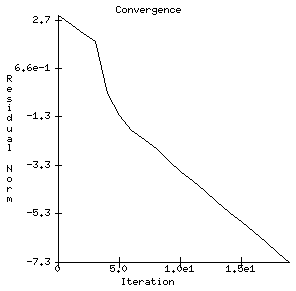
\includegraphics[width=0.9\textwidth]{line-graph-c1tri}
\caption{\PETSc can use X windows to produce line graphs at run time.  (This is not to say they are pretty.)}
\label{fig:line-graph-c1tri}
\end{marginfigure}

Finally, \PETSc can generate graphics showing convergence of iterative methods, at least if X windows are installed.  The line graph in Figure \ref{fig:line-graph-c1tri}, from
\begin{cline}
$ ./c1tri -tri_m 1000000 -ksp_rtol 1.0e-10 -pc_type jacobi \
    -ksp_monitor_lg_residualnorm -draw_pause 1
\end{cline}
%$
shows the residual norm logarithm versus the iteration number.

\bigskip
\section{Exercises}

\renewcommand{\labelenumi}{\arabic{chapter}.\arabic{enumi}\quad}
\begin{enumerate}
\item Show \eqref{introconvergethm}.
\item As the reader will undoubtedly experience, segmentation faults and memory leaks are inevitable when one develops \PETSc codes.  A standard tool for detecting/diagnosing these is \texttt{valgrind}.\sidenote{\href{http://valgrind.org/}{valgrind.org}}  We recommend running it frequently.  As an exercise, run
\begin{cline}
valgrind ./c1vecmatksp
\end{cline}
to see what \texttt{valgrind} shows for a leak-free program.  Then comment-out a \texttt{VecDestroy()} call in \texttt{c1vecmatksp.c} and rerun to see a common type of memory leak.
\item Consider Richardson iteration in the example
\begin{cline}
./c1tri -tri_m 100 -ksp_monitor -ksp_type richardson
\end{cline}
Un-preconditioned Richardson iteration fails (i.e.~add \texttt{-pc\_type none}); explain.  The default preconditioner succeeds (i.e.~\texttt{-pc\_type ilu}), but ILU($0$) is cheating because it becomes a complete LU factorization on this tridiagonal and diagonally-dominant $A$; we are really seeing a direct solve.  The same can be said for ICC($0$).  Confirm that, as in the example on page \pageref{introprerichardson}, Richardson iteration succeeds with \texttt{-pc\_type jacobi}, even though the diagonal is constant; explain.
\item \label{exer:computeeigs} Un-preconditioned GMRES solves the linear system in \texttt{c1tri.c} reasonably efficiently.  We can explain this by asking \PETSc to compute the eigenvalues of $A$ by using option\sidenote{The relevant \PETSc manual page says this option is ``intended only for assistance in understanding the convergence of iterative methods, not for eigenanalysis.  For accurate computation of eigenvalues we recommend using the excellant package SLEPc.''}
\begin{quote}
\texttt{-ksp\_compute\_eigenvalues}
\end{quote}
Because otherwise it computes the eigenvalues of the preconditioned operator $P^{-1}A$, add \texttt{-pc\_type none}.  Try dimensions $N=10,100,1000$.  Why does the  run
\begin{cline}
./c1tri -tri_n 1000 -pc_type none -ksp_compute_eigenvalues
\end{cline}
only show 11 eigenvalues of this $1000\times 1000$ matrix?  How do these eigenvalues explain the good behavior of unpreconditioned GMRES?\sidenote{See \citep{TrefethenBau} for help with both of these questions.}
\item The accuracy of direct solves (e.g.~\texttt{-ksp\_type preonly -pc\_type cholesky}) in \texttt{c1tri.c}, as measured by the reported error norm $\|\bx - \bx_{\text{exact}}\|_2$, decreases with increasing dimension.  Confirm and explain this observation.
\item Table \ref{tab:c1tritiming} includes a number of blanks.  For each one, explain why it is blank, experimenting if needed.
\item Table \ref{tab:c1tritiming} gives execution times not iteration count.  Generate the corresponding table of \pKSP iteration count by adding option \verb|-ksp_converged_reason| to the run commands.  Note the large number of ``coincidences'' in iteration count, i.e.~cases where iteration counts are identical; explain.  Which preconditioners have a strong or weak effect on iteration count?  Is timing or iteration count more useful?
\end{enumerate}

\chapter{Poisson equation on a structured grid}
\label{chap:st}
\renewcommand{\CODELOC}{ch3/}

\chapter{2. Linear PDEs: a structured grid example}

We start with the Poisson problem because it is the right place to start.  Though it is a cliche in applied mathematics, in solving it we will use key parts of \PETSc: build a structured grid using a \PETSc \pDMDA, assemble a \pMat and some \pVecs in parallel on this grid, and solve in parallel using a \pKSP object.

\section{A Poisson problem on a square domain}

The \emph{Laplacian}
    $$\grad^2 u = \Div(\grad u) = \frac{\partial^2 u}{\partial x^2} + \frac{\partial^2 u}{\partial y^2}$$
of a function $u(x,y)$ almost always appears in a mathematical model because the quantity $u$ is conserved in some sense, and because of an assumption that the gradient $\grad u$ is, up to a coefficient, the flux of $u$ \citep{Ockendonetal2003}.  The divergence ``$\Div$'' factor arises from a connection between a flux integral over a closed surface and an integral over the interior of that surface, namely the divergence (Gauss-Green) theorem \citep[Appendix C]{Evans}.

In the \emph{Poisson equation} the Laplacian of $u$ is equal to a known function.  We will not just solve this one equation on a finite region, however.  We solve a \emph{Poisson problem} including boundary conditions, and the whole problem determines a solution which we will approximate numerically.  Let $\mathcal{S}$ be the open unit square $(0,1)\times(0,1)$.  The following is our Poisson problem for this Chapter;  see Figure \ref{fig:unitsquare}:
\begin{marginfigure}
\begin{tikzpicture}[scale=3.5]
  \draw[->,gray,very thin] (-0.2,0.0) -- (1.2,0.0) node[below] {$x$};
  \draw[->,gray,very thin] (0.0,-0.2) -- (0.0,1.2) node[left] {$y$};
  \draw[line width=1.0pt] (0.0,0.0) -- (0.0,1.0) -- (1.0,1.0) -- (1.0,0.0) -- cycle;
  \node at (0.5,0.5) {$- \grad^2 u = f$};
  \node at (0.5,-0.1) {$u = 0$};
  \node at (0.5,1.1) {$u = 0$};
  \node at (-0.2,0.5) {$u = 0$};
  \node at (1.2,0.5) {$u = 0$};
\end{tikzpicture}
\caption{Our first, simple goal is to solve the Poisson equation on the unit square $\mathcal{S}$, with homogeneous Dirichlet boundary conditions.}
\label{fig:unitsquare}
\end{marginfigure}
\begin{align}
- \grad^2 u &= f \quad \text{ on } \mathcal{S}, \label{poissonsquare} \\
u &= 0 \quad \text{ on } \partial \mathcal{S}. \notag
\end{align}
The boundary of the unit square, denoted ``$\partial\mathcal{S}$'', is simply the union of four (closed) line segments.  The boundary conditions $u=0$ are called ``\emph{homogeneous Dirichlet}.''

The Poisson problem can model the electrostatic potential, the equilibrium distribution from certain random walks, the distribution of temperature in a conducting object at steady state, and many other other physical phenomena.  For example, in the context of heat conduction Fourier's law says $\bq = -k \grad u$, where $k$ is approximately constant if the variation in $u$ is not too large.  Conservation of energy for a solid says $c\rho \partial u/\partial t = - \Div\bq + f$ if $f$ describes a heat source within the domain.  At steady state these facts combine to give $0 = k \grad^2 u + f$, that is, Poisson's equation \eqref{poissonsquare}.  Holding the temperature fixed at zero along the boundary completes the problem.

For this chapter we will suppose that $f(x,y)$ is continuous and bounded on $\mathcal{S}$, so that we can compute its pointwise values.  With our homogeneous Dirichlet boundary conditions, and the assumptions on $f$, standard theory says that $u(x,y)$ exists and is continuous on the closed square $\overline{\mathcal{S}}$ \citep[Theorem 6 in section 5.6]{Evans}.\sidenote{A classical approach to showing existence starts by solving problem \eqref{poissonsquare} by Fourier series.  If $f$ is square-integrable then the coefficients $\hat f$ are square-integrable (Parseval's equality).  Because the Laplacian is elliptic and second-order, the coefficients $\hat u$ are square-integrable even when multiplied by the frequency squared.  By Cauchy-Schwarz, the Fourier series for $u$ is the limit of a sequence of continuous functions on $\overline{\mathcal{S}}$ which converge uniformly, so $u\in C^0(\overline{\mathcal{S}})$.}  Thus there is no ambiguity in the boundary condition ``$u=0$ on $\partial \mathcal{S}$,'' and also we can sensibly discuss the pointwise values $u(x,y)$.

Without any boundary conditions, the Poisson equation $-\grad^2 u = f$ alone is not a well-posed problem because if $u$ is a solution then $v=u+C$ is also a solution for any constant $C$.  (In fact there are constant solutions $w=C$ and many, many more to the Laplace equation $-\grad^2 w = 0$ on $\mathcal{S}$.)  However, with the Dirichlet boundary conditions in \eqref{poissonsquare}, the solution is unique if it exists \citep[Theorem 5 in section 2.2]{Evans}; \citep[subsection 5.2.1]{Ockendonetal2003}.


\section{A finite difference method: build the grid}

Because \eqref{poissonsquare} is a linear problem, finite-dimensional approximations of it are simply linear systems.  The finite-dimensional approximation in this Chapter comes from applying a \emph{finite difference} (FD) method.  In Chapter 3 we will apply a finite element approach instead.

\begin{marginfigure}
\begin{tikzpicture}[scale=3.5]
  \draw[->,gray,very thin] (0.0,0.0) -- (1.2,0.0) node[below] {$x$};
  \draw[->,gray,very thin] (0.0,0.0) -- (0.0,1.2) node[left] {$y$};
  \draw[line width=1.0pt] (0.0,0.0) -- (0.0,1.0) -- (1.0,1.0) -- (1.0,0.0) -- cycle;
  \node at (0.0,-0.1) {$i=0$};
  \node at (1.0,-0.1) {$i=M-1$};
  \node at (-0.15,0.0) {$j=0$};
  \node at (-0.22,1.0) {$j=N-1$};
  \pgfmathsetmacro\fourth{1.0/4.0}
  \pgfmathsetmacro\sixth{1.0/6.0}
  \draw[xstep=\fourth,ystep=\sixth,black,thin] (0.0,0.0) grid (1.0,1.0);
\end{tikzpicture}
\caption{A grid on the unit square $\mathcal{S}$, with $M=5$ and $N=7$.}
\label{fig:unitsquaregrid}
\end{marginfigure}

To start our FD method we put a \emph{structured grid} of $MN$ points on the unit square, as in Figure \ref{fig:unitsquaregrid}, with spacing $h_x=1/(M-1)$ and $h_y=1/(N-1)$ in the two directions.  The grid locations are $x_i = i\, h_x$ for $i = 0,1,\dots,M-1$ and $y_j = j\, h_y$ and $j=0,1,\dots,N-1$.

The construction of such a two-dimensional (2D) grid, and the distribution of it across processors, will be our first new idea from \PETSc, beyond the basics in Chapter 1.  Consider the lines of code in Figure \ref{code:dmdacreatetwod}.  They create a \PETSc \pDM object\sidenote{``\pDM'' might stand for ``data management'', but perhaps ``distributed mesh'' is better.} for a grid like Figure \ref{fig:unitsquaregrid}.

\clearpage
\cinputraw{dmdacreate2d.frag}{extract from c2poisson.c}{An example of creating a 2D \pDMDA.}{}{//START}{//STOP}{code:dmdacreatetwod}

A \pDM is an abstract type for describing the topology (i.e.~connectedness) of a grid, \emph{and} the way it is distributed across \MPI processes, \emph{and} the way each process can access data from its neighbors.  The specific variable \texttt{da} in Figure \ref{code:dmdacreatetwod} has type ``\pDMDA'', which is the subclass of \pDM s which are structured grids.

The Figure \ref{code:dmdacreatetwod} code will appear in \texttt{c2poisson.c} below, which solves Poisson's problem.  For now, if we do
\begin{Verbatim}[fontsize=\small]
  make c2poisson
  mpiexec -n 4 ./c2poisson -da_grid_x 5 -da_grid_y 7
\end{Verbatim}
then a structured grid will be distributed across the four processes exactly as in Figure \ref{fig:unitsquaregridparallel}.  Neither $M=5$ nor $N=7$ is divisible by two in this case, but \PETSc distributes the four ranks across the $MN=35$ nodes (grid points) as uniformly as possible given that each processor owns a rectangular subgrid.  In fact, the rank $0$ process has the most nodes (12) and rank $3$ has the least (6), so the load is only uniform within a factor of two, but larger grids will be better load-balanced.  \PETSc does the best it can.

\begin{marginfigure}
\begin{tikzpicture}[scale=3.5]
  \draw[->,gray,very thin] (0.0,0.0) -- (1.2,0.0) node[below] {$x$};
  \draw[->,gray,very thin] (0.0,0.0) -- (0.0,1.2) node[left] {$y$};
  \draw[line width=1.0pt] (0.0,0.0) -- (0.0,1.0) -- (1.0,1.0) -- (1.0,0.0) -- cycle;
  \pgfmathsetmacro\fourth{1.0/4.0}
  \pgfmathsetmacro\sixth{1.0/6.0}
  \draw[xstep=\fourth,ystep=\sixth,black,thin] (0.0,0.0) grid (1.0,1.0);
  \pgfmathsetmacro\dd{0.04}
  \pgfmathsetmacro\od{1.04}
  \pgfmathsetmacro\xap{2*\fourth + 0.04}
  \pgfmathsetmacro\xbm{3*\fourth - 0.04}
  \pgfmathsetmacro\yap{3*\sixth + 0.04}
  \pgfmathsetmacro\ybm{4*\sixth - 0.04}
  \pgfmathsetmacro\xamid{1*\fourth}
  \pgfmathsetmacro\xbmid{3.5*\fourth}
  \pgfmathsetmacro\yamid{1.5*\sixth}
  \pgfmathsetmacro\ybmid{5*\sixth}
  \draw[thick,rounded corners=8pt,color=red]
    (-\dd,-\dd) -- (-\dd,\yap) -- (\xap,\yap) -- (\xap,-\dd) -- cycle;
  \node[color=red] at (\xamid,\yamid) {rank $0$};
  \draw[thick,rounded corners=8pt,color=red]
    (\xbm,-\dd) -- (\od,-\dd) -- (\od,\yap) -- (\xbm,\yap) -- cycle;
  \node[color=red] at (\xbmid,\yamid) {rank $1$};
  \draw[thick,rounded corners=8pt,color=red]
    (-\dd,\ybm) -- (\xap,\ybm) -- (\xap,\od) -- (-\dd,\od) -- cycle;
  \node[color=red] at (\xamid,\ybmid) {rank $2$};
  \draw[thick,rounded corners=8pt,color=red]
    (\xbm,\ybm) -- (\od,\ybm) -- (\od,\od) -- (\xbm,\od) -- cycle;
  \node[color=red] at (\xbmid,\ybmid) {rank $3$};
\end{tikzpicture}
\caption{The same grid as in Figure \ref{fig:unitsquaregrid}, distributed across four \MPI processes (i.e.~with \texttt{rank} $\in \{0,1,2,3\}$) automatically by \texttt{DMDACreate2d()}.}
\label{fig:unitsquaregridparallel}
\end{marginfigure}

The fifth and sixth arguments ``\texttt{-10}'' to \texttt{DMDACreate2d()} in Figure \ref{code:dmdacreatetwod} are used to set default dimensions $M=10$ and $N=10$.  We have seen that these defaults are overridden by runtime options \texttt{-da\_grid\_x} and \texttt{-da\_grid\_y}.  However, if we do this,
 \begin{Verbatim}[fontsize=\small]
  mpiexec -n 4 ./c2poisson
\end{Verbatim}
then a structured grid will be distributed across the four processes as in Figure \ref{fig:unitsquaregrideight}, with each rank owning 25 nodes.  \PETSc itself can show the parallel layout by calling
\begin{Verbatim}[fontsize=\small]
  mpiexec -n 4 ./c2poisson -dm_view
\end{Verbatim}
or
\begin{Verbatim}[fontsize=\small]
  mpiexec -n 4 ./c2poisson -dm_view draw -draw_pause 2
\end{Verbatim}
The latter version shows the grid graphically, for two seconds.

\begin{marginfigure}
\begin{tikzpicture}[scale=3.5]
  \draw[->,gray,very thin] (0.0,0.0) -- (1.2,0.0) node[below] {$x$};
  \draw[->,gray,very thin] (0.0,0.0) -- (0.0,1.2) node[left] {$y$};
  \draw[line width=1.0pt] (0.0,0.0) -- (0.0,1.0) -- (1.0,1.0) -- (1.0,0.0) -- cycle;
  \pgfmathsetmacro\ninth{1.0/9.0}
  \draw[xstep=\ninth,ystep=\ninth,black,thin] (0.0,0.0) grid (1.0,1.0);
  \pgfmathsetmacro\dd{0.04}
  \pgfmathsetmacro\od{1.04}
  \pgfmathsetmacro\ap{4*\ninth + 0.04}
  \pgfmathsetmacro\bm{5*\ninth - 0.04}
  \pgfmathsetmacro\amid{2*\ninth}
  \pgfmathsetmacro\bmid{7*\ninth}
  \draw[thick,rounded corners=8pt,color=red]
    (-\dd,-\dd) -- (-\dd,\ap) -- (\ap,\ap) -- (\ap,-\dd) -- cycle;
  \node[color=red] at (\amid,\amid) {rank $0$};
  \draw[thick,rounded corners=8pt,color=red]
    (\bm,-\dd) -- (\od,-\dd) -- (\od,\ap) -- (\bm,\ap) -- cycle;
  \node[color=red] at (\bmid,\amid) {rank $1$};
  \draw[thick,rounded corners=8pt,color=red]
    (-\dd,\bm) -- (\ap,\bm) -- (\ap,\od) -- (-\dd,\od) -- cycle;
  \node[color=red] at (\amid,\bmid) {rank $2$};
  \draw[thick,rounded corners=8pt,color=red]
    (\bm,\bm) -- (\od,\bm) -- (\od,\od) -- (\bm,\od) -- cycle;
  \node[color=red] at (\bmid,\bmid) {rank $3$};
\end{tikzpicture}
\caption{An $M=10$ by $N=10$ grid distributed by \texttt{DMDACreate2d()} across four \MPI processes.}
\label{fig:unitsquaregrideight}
\end{marginfigure}

To explain the other options to \texttt{DMDACreate2d()} used in Figure \ref{code:dmdacreatetwod}, we quote the \PETSc manual pages description of that method:

\clearpage
\noindent\hrulefill
\begin{Verbatim}[fontsize=\small]
DMDACreate2d(MPI_Comm comm, DMBoundaryType bx, DMBoundaryType by,
  DMDAStencilType stype, PetscInt M, PetscInt N, PetscInt m, PetscInt n,
  PetscInt dof, PetscInt s, const PetscInt lx[], const PetscInt ly[],
  DM *da)
\end{Verbatim}
where
\small
\begin{itemize}[align=left]
\item[\texttt{comm}]   MPI communicator \\
\item[\texttt{bx,by}]  type of ghost nodes the array have; use one of \texttt{DM\_BOUNDARY\_NONE, DM\_BOUNDARY\_GHOSTED, DM\_BOUNDARY\_PERIODIC} \\
\item[\texttt{stype}] stencil type; use either \texttt{DMDA\_STENCIL\_BOX} or \texttt{DMDA\_STENCIL\_STAR} \\
\item[\texttt{M,N}]	   global dimension in each direction of the array; use \texttt{-M} and or \texttt{-N} to indicate that it may be set to a different value from the command line with \texttt{-da\_grid\_x <M> -da\_grid\_y <N>} \\
\item[\texttt{m,n}]   corresponding number of processors in each dimension (or \texttt{PETSC\_DECIDE} to have calculated) \\
\item[\texttt{dof}]     number of degrees of freedom per node \\
\item[\texttt{s}]       stencil width \\
\item[\texttt{lx,ly}]  arrays containing the number of nodes in each cell along the x and y coordinates, or \texttt{NULL}; if non-null, these must be of length as m and n, and the corresponding m and n cannot be \texttt{PETSC\_DECIDE}; the sum of the \texttt{lx[]} entries must be M, and the sum of the \texttt{ly[]} entries must be N \\
\item[\texttt{da}]      output: the resulting distributed array object 
\end{itemize}
\normalsize
\noindent\hrulefill
\medskip

In Figure \ref{code:dmdacreatetwod}, the first argument is a serial or parallel \MPI communicator.  In the second and third arguments we have used ``\texttt{DM\_BOUNDARY\_NONE}'' because our Dirichlet boundary condition does not require communication to the next process' domain, nor periodic wrapping.  In the fourth argument we use \texttt{DMDA\_STENCIL\_STAR} because only cardinal neighbors of a grid point are used when forming the matrix; we will address the FD ``stencil'' below.  As already noted, the fifth and sixth arguments set $M=10,N=10$ as override-able grid defaults.  In the next two arguments we indeed use ``\texttt{PETSC\_DECIDE}'' to have \PETSc parallel-decompose our grid according to the size of (i.e.~number of processes in) the \MPI communicator.  The next two arguments, in the ninth and tenth positions, say that our PDE is scalar (\texttt{dof}$=1$) and that the FD method only needs one neighbor in each direction (\texttt{s}$=1$).  The next two arguments are \texttt{NULL} because we are \emph{not} telling \PETSc how to distribute processes over the grid; it \texttt{DECIDE}s for itself.  Finally, the \pDMDA object is created as an output.

The call to \texttt{DMDASetUniformCoordinates()} in Figure \ref{code:dmdacreatetwod} sets the domain to be $[0,1]\times[0,1]$.  The last two arguments are ignored in this case but would set limits on the third dimension in 3D.

To wrap up our coverage of creating grids, the standard \PETSc view of what \pDM s ``look like'' is in Figure \ref{fig:petscghostvalues}.  On the left is a version of what we have done in the code in Figure \ref{code:dmdacreatetwod}, namely create a structured grid \pDM.  The one shown in Figure \ref{fig:petscghostvalues} has \texttt{DMDA\_STENCIL\_BOX} stencil type, unlike ours.  On the right is an unstructured grid, of the type created in Chapter 3 for the finite element method.  In both cases the figure shows nodes owned by a given process (red ``local'' nodes) and those other nodes that are accessible by the local process (blue ``ghost'' nodes).  We will see such local/ghost node types in all examples in this book.

\begin{figure}
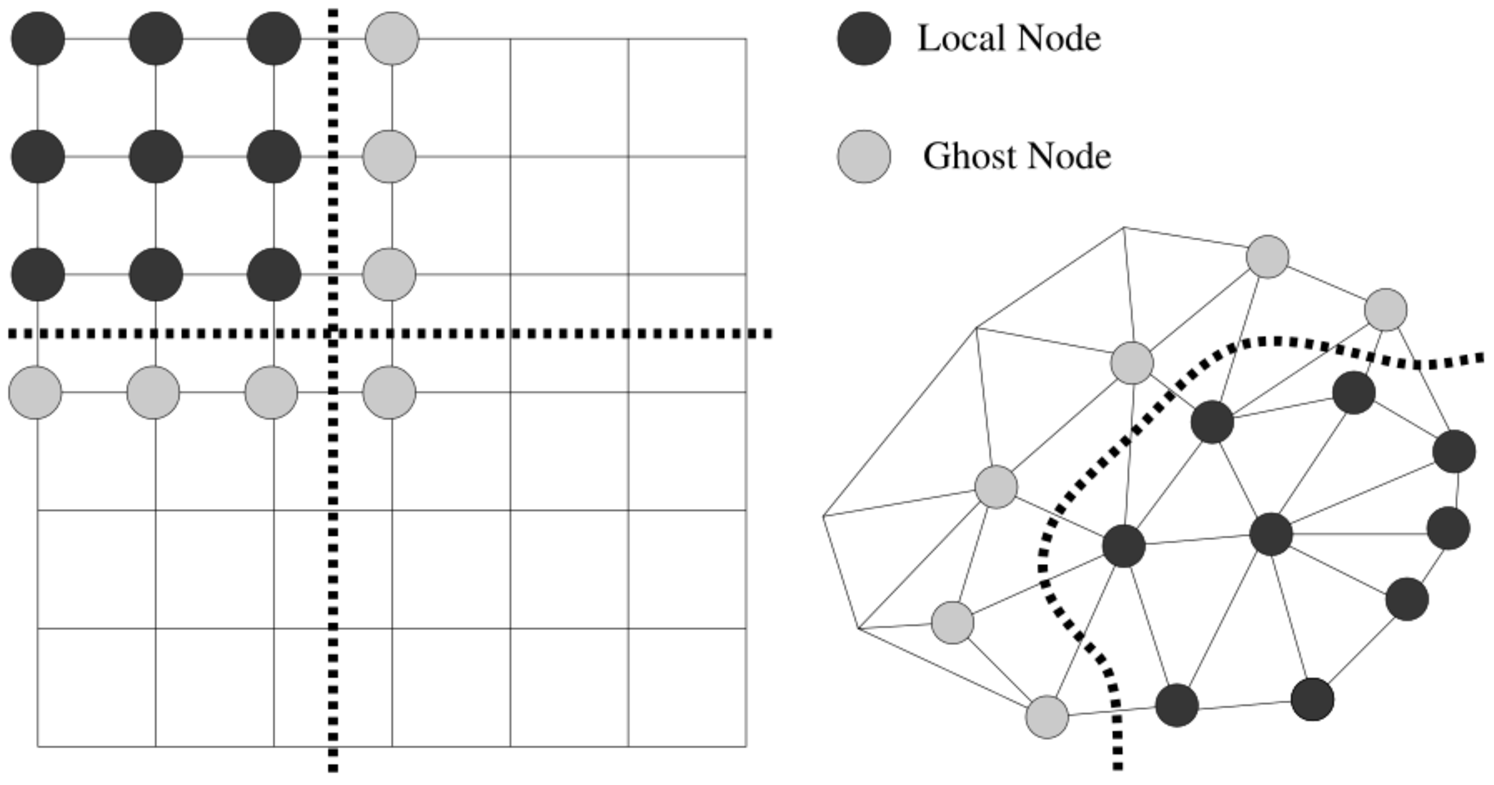
\includegraphics[width=\textwidth]{petscghostvalues}
\caption{\PETSc's parallel decomposition of structured and unstructured grids, showing owned (``local'') and accessible (``ghost'') nodes for one process.}
\label{fig:petscghostvalues}
\end{figure}


\section{A finite difference method: assemble the linear system}

Recall we were trying to approximate PDE problem \eqref{poissonsquare}.  Having built a structured grid we can now return to the FD method.

By a well-known Taylor's theorem argument \citep{MortonMayers}, for any function $F(x)$ which is sufficiently smooth, we have
    $$F''(x) = \frac{F(x+h) - 2 F(x) + F(x-h)}{h^2} + O(h^2)$$
as $h$ goes to zero.  This formula, applied to partial derivatives, will give an approximation of the Laplacian in problem \eqref{poissonsquare}.

Let $U_{i,j}$ be the gridded approximation to the exact value $u(x_i,y_j)$ of the solution $u$,\sidenote{This is an important sentence!  We \emph{compute} values $U_{i,j}$ from the finite difference equations.  We generally \emph{don't know} the values of the exact solution on the grid, namely $u(x_i,y_j)$.  Of course we want the former to be close to the latter.}  and also denote $f_{i,j} = f(x_i,y_j)$.  Then we have this FD approximation to problem \eqref{poissonsquare}:
\begin{equation}
- \frac{U_{i+1,j} - 2 U_{i,j} + U_{i-1,j}}{h_x^2} - \frac{U_{i,j+1} - 2 U_{i,j} + U_{i,j-1}}{h_y^2} = f_{i,j}. \label{poissonsquareFDearly}
\end{equation}
Equation \eqref{poissonsquareFDearly} applies for all of the interior points where $1 \le i \le M-2$ and $1 \le j \le N-2$.  The boundary conditions in \eqref{poissonsquare} become
\begin{equation}
U_{0,j} = 0, \quad U_{M-1,j} = 0, \quad U_{i,0} = 0, \quad U_{i,N-1} = 0, \label{poissonsquareFDbcs}
\end{equation}
for all $i,j$.

At location $(x_i,y_j)$, equation \eqref{poissonsquareFDearly} relates the unknown $U_{i,j}$ to its four cardinal neighbors $U_{i+1,j}$, $U_{i-1,j}$, $U_{i,j+1}$, and $U_{i,j-1}$.  This pattern is a \emph{stencil}, in particular a ``star'' stencil, as shown in Figure \ref{fig:unitsquaregridstencil}.  A ``box'' stencil would also involve all the diagonal neighbors, so an equation using a star stencil relates at most five unknowns in 2D, while one with a box stencil relates at most nine unknowns in 2D.

\begin{marginfigure}
\begin{tikzpicture}[scale=3.5]
  \draw[->,gray,very thin] (0.0,0.0) -- (1.2,0.0) node[below] {$x$};
  \draw[->,gray,very thin] (0.0,0.0) -- (0.0,1.2) node[left] {$y$};
  \draw[line width=1.0pt] (0.0,0.0) -- (0.0,1.0) -- (1.0,1.0) -- (1.0,0.0) -- cycle;
  \node at (0.75,-0.1) {$i$};
  \node at (-0.1,0.666667) {$j$};
  \filldraw (0.50,0.666667) circle (0.8pt);
  \filldraw (0.75,0.666667) circle (0.8pt);
  \filldraw (1.00,0.666667) circle (0.8pt);
  \filldraw (0.75,0.5) circle (0.8pt);
  \filldraw (0.75,0.833333) circle (0.8pt);
  \draw[line width=2.0pt] (0.50,0.666667) -- (1.00,0.666667);
  \draw[line width=2.0pt] (0.75,0.5)  -- (0.75,0.833333);
  \draw[xstep=0.25,ystep=0.166667,black,thin] (0.0,0.0) grid (1.0,1.0);
\end{tikzpicture}
\caption{A ``star'' stencil, shown on the same grid as in Figure \ref{fig:unitsquaregrid}, at $i=3$ and $j=4$.}
\label{fig:unitsquaregridstencil}
\end{marginfigure}

Equations \eqref{poissonsquareFDearly} and \eqref{poissonsquareFDbcs} form a linear system of $K=MN$ equations in which we choose to treat all $K$ locations on the grid as unknowns.  To shown this linear system in traditional form
\begin{equation}
A \bu = \bb,
\end{equation}
where $A$ is a $K\times K$ matrix and $\bu,\bb$ are $K\times 1$ column vectors, we must order the unknowns.  This ordering will be used internally by \PETSc in a code that uses a \pDMDA, and we use it here for displaying the system, but the code we will actually write uses the grid-wise coordinates $(i,j)$.  One could write this ordering as
\begin{equation}
    U_k = U_{i,j} \quad \text{ where } \quad k = j\,M + i. \label{orderingfd}
\end{equation}
We will let \PETSc do such index transformations internally, because, as we will see, it has tools for $i,j$-type indexing.  Now is a good time to show the linear system itself, and the ordering, in a small case.

\begin{marginfigure}
\begin{tikzpicture}[scale=3.5]
  \draw[->,gray,very thin] (0.0,0.0) -- (1.2,0.0) node[below] {$x$};
  \draw[->,gray,very thin] (0.0,0.0) -- (0.0,1.2) node[left] {$y$};
  \draw[line width=1.0pt] (0.0,0.0) -- (0.0,1.0) -- (1.0,1.0) -- (1.0,0.0) -- cycle;
  \pgfmathsetmacro\third{1.0/3.0}
  \pgfmathsetmacro\half{1.0/2.0}
  \node at (0.0,-0.1) {$0$};
  \node at (\third,-0.1) {$1$};
  \node at (\half,-0.2) {$i$};
  \node at (2*\third,-0.1) {$2$};
  \node at (1.0,-0.1) {$3$};
  \node at (-0.1,0.0) {$0$};
  \node at (-0.1,0.5) {$1$};
  \node at (-0.25,0.5) {$j$};
  \node at (-0.1,1.0) {$2$};
  \draw[xstep=\third,ystep=\half,black,thin] (0.0,0.0) grid (1.0,1.0);
  \pgfmathsetmacro\dd{0.04}
  \foreach \y in {0,1,2}
    \foreach \x in {0,1,2,3} {
      \pgfmathsetmacro\k{4*\y+\x}
      \draw[color=blue] (\x*\third+\dd,\y*\half+\dd) node{\pgfmathprintnumber[fixed]{\k}};
    }
\end{tikzpicture}
\caption{Ordering of unknowns \eqref{orderingfd} on a $M=4$ and $N=3$ grid.  Index $k = j\,M + i$ is shown in {\color{blue} blue}.}
\label{fig:unitsquaregridordering}
\end{marginfigure}

\medskip\noindent\hrulefill
\begin{example} In the $M=4$ and $N=3$ case we have the grid and variable ordering shown in Figure \ref{fig:unitsquaregridordering}.  Note $h_x=1/3$ and $h_y=1/2$.  Equations \eqref{poissonsquareFDearly} and \eqref{poissonsquareFDbcs} are an invertible system of $K=12$ equations.  Only the $k=5$ and $k=6$ equations are not boundary conditions \eqref{poissonsquareFDbcs}:
\setcounter{MaxMatrixCols}{20}
\begin{equation*}
\begin{bmatrix}
1 &  &  &  &  &  &  &  &  &  &  &  \\
  & 1&  &  &  &  &  &  &  &  &  &  \\
  &  & 1&  &  &  &  &  &  &  &  &  \\
  &  &  & 1&  &  &  &  &  &  &  &  \\
  &  &  &  & 1&  &  &  &  &  &  &  \\
  & c&  &  & b& a& b&  &  & c&  &  \\
  &  & c&  &  & b& a& b&  &  & c&  \\
  &  &  &  &  &  &  & 1&  &  &  &  \\
  &  &  &  &  &  &  &  & 1&  &  &  \\
  &  &  &  &  &  &  &  &  & 1&  &  \\
  &  &  &  &  &  &  &  &  &  & 1&  \\
  &  &  &  &  &  &  &  &  &  &  & 1
\end{bmatrix}
\begin{bmatrix}
U_{0,0} \\
U_{1,0} \\
U_{2,0} \\
U_{3,0} \\
U_{0,1} \\
U_{1,1} \\
U_{2,1} \\
U_{3,1} \\
U_{0,2} \\
U_{1,2} \\
U_{2,2} \\
U_{3,2}
\end{bmatrix}
=
\begin{bmatrix}
0 \\
0 \\
0 \\
0 \\
0 \\
f_{1,1} \\
f_{2,1} \\
0 \\
0 \\
0 \\
0 \\
0
\end{bmatrix}
\end{equation*}
where $a = 2/h_x^2 + 2/h_y^2 = 26$, $b = - 1/h_x^2 = -9$ and $c = - 1/h_y^2 = -4$.

Note that the matrix $A$ is not symmetric, and it is not well-scaled for such a small example.  For instance, its 2-norm condition number \citep{TrefethenBau} is $\cond(A) = \|A\|_2 \|A^{-1}\|_2 = 43.16$.
\end{example}
\noindent\hrulefill

Before assembling the system, by writing \PETSc code, there are two nontrivial observations about it.  First, the equations \eqref{poissonsquareFDearly} have very different ``scaling'' from those in \eqref{poissonsquareFDbcs}.  For example, if $M=N=1001$, so that $h_x=h_y=0.001$, then the coefficient of $U_{i,j}$ in \eqref{poissonsquareFDearly} is $4/(.001)^2 = 4 \times 10^6$, where as the coefficients of $U_{i,j}$ along the boundary in \eqref{poissonsquareFDbcs} are equal to 1.  Therefore we multiply equation \eqref{poissonsquareFDearly} by the grid cell area $h_x h_y$ to get
\begin{align}
&\left(2 \frac{h_y}{h_x} + 2 \frac{h_x}{h_y}\right) U_{i,j} - \frac{h_y}{h_x}\left(U_{i+1,j} + U_{i-1,j}\right)  - \frac{h_x}{h_y}\left(U_{i,j+1} + U_{i,j-1}\right) \label{poissonsquareFD} \\
&\qquad = h_x h_y f_{i,j}. \notag
\end{align}
Using \eqref{poissonsquareFD}, as long as the cell aspect ratio $\max\{h_y/h_x,h_x/h_y\}$ is not too large, all the equations in the system, including the boundary conditions, will have coefficients of comparable size.  Note that if $h_x=h_y$ then the diagonal entries are equal to $4$ and the off-diagonal entries are $-1$.

Second, our equations can be interpreted to give a \emph{symmetric} matrix $A$.  This opens up a larger range of linear algebra methods for solving the system efficiently.  For example, in the $i=1$ case of \eqref{poissonsquareFD}, i.e.~at a grid point adjacent to the left-hand boundary of the square, the boundary location value $U_{0,j}$ appears in the equation.  The matrix in the linear system will be symmetric if we systematically ``move'' such values to the right-hand side as known (and zero) instead of inserting a ``$1$'' into the corresponding matrix locations.  That is, we make off-diagonal zero entries in the columns corresponding to known boundary values, in addition to the off-diagonal zeros in rows corresponding to known boundary values.  With these two modifications we can redo the above $M=4$ and $n=3$ example.

\medskip\noindent\hrulefill
\begin{example} For the same $M=4$ and $N=3$ case shown in Figure \ref{fig:unitsquaregridordering}, equations \eqref{poissonsquareFDbcs} and \eqref{poissonsquareFD} become
\begin{equation*}
\begin{bmatrix}
1 &  &  &  &  &  &  &  &  &  &  &  \\
  & 1&  &  &  &  &  &  &  &  &  &  \\
  &  & 1&  &  &  &  &  &  &  &  &  \\
  &  &  & 1&  &  &  &  &  &  &  &  \\
  &  &  &  & 1&  &  &  &  &  &  &  \\
  &  &  &  &  & \alpha& \beta&  &  &  &  &  \\
  &  &  &  &  & \beta& \alpha&  &  &  &  &  \\
  &  &  &  &  &  &  & 1&  &  &  &  \\
  &  &  &  &  &  &  &  & 1&  &  &  \\
  &  &  &  &  &  &  &  &  & 1&  &  \\
  &  &  &  &  &  &  &  &  &  & 1&  \\
  &  &  &  &  &  &  &  &  &  &  & 1
\end{bmatrix}
\begin{bmatrix}
U_{0,0} \\
U_{1,0} \\
U_{2,0} \\
U_{3,0} \\
U_{0,1} \\
U_{1,1} \\
U_{2,1} \\
U_{3,1} \\
U_{0,2} \\
U_{1,2} \\
U_{2,2} \\
U_{3,2}
\end{bmatrix}
=
\begin{bmatrix}
0 \\
0 \\
0 \\
0 \\
0 \\
(1/6) f_{1,1} \\
(1/6) f_{2,1} \\
0 \\
0 \\
0 \\
0 \\
0
\end{bmatrix}
\end{equation*}
where $\alpha = 2 (h_y/h_x) + 2 (h_x/h_y) = 13/3$ and $\beta = - h_y/h_x = 3/2$.  The matrix is better-scaled, with $\cond(A)=5.83$.
\end{example}
\noindent\hrulefill


FIXME: explain Mat assembly tools, including DALocalInfo and MatStencil

\clearpage

\cinput{structuredlaplacian.c}{Fill matrix entries using \texttt{MatSetValuesStencil}.}{//CREATEMATRIX}{//ENDCREATEMATRIX}{code:structuredlaplacian}

\cinputpart{c2poisson.c}{The right side of equation \eqref{poissonsquareFD} comes from differentiating the exact solution, which this method also computes.}{I}{//RHS}{//ENDRHS}{code:ctwopoissonrhs}

\cinputpart{c2poisson.c}{Set up \pDMDA \texttt{da} and \pMat \texttt{A} objects, and assemble the latter by calling \texttt{formlaplacian()}.}{II}{//CREATE}{//ENDCREATE}{code:ctwopoissoncreate}

\cinputpart{c2poisson.c}{Solve using \pKSP, and report on solution.}{III}{//SOLVE}{//ENDSOLVE}{code:ctwopoissonsolve}

\section{Runtime control of linear solver}

FIXME: basic Krylov theory

\section{Time-dependent heat equation}

FIXME: we WON'T do explicit, but it would look like ...

FIXME: use TS for backward-euler


\chapter{Nonlinear equations}
\label{chap:nl}
\renewcommand{\CODELOC}{ch4/}

The simplest thing to say about nonlinear equations is that they change change the functional form of the residual, compared to the linear case.  For a linear system the residual $\br$, defined in \eqref{residualdefn}, is a certain function of the unknowns $\bu$, namely
\begin{equation}
\bF(\bu) = \bb - A \bu. \label{eq:nl:linres}
\end{equation}
Now we consider cases in which $\bF$ is a higher-order polynomial, a transcendental function, or some more general function.

In fact, let us simply suppose for now that $\bF : \RR^N \to \RR^N$ is differentiable.  The input $\bx$ and output $\bF(\bx)$ are column vectors,\sidenote{Our name change $\bu\to\bx$, relative to \eqref{eq:nl:linres}, comes from thinking more geometrically about changes in the location of $\bx$.} so in that sense $\bF$ acts like square-matrix multiplication $\bx\mapsto A\bx$.  A linear solver like GMRES (Chapter \ref{chap:ls}) reduces the residual \eqref{eq:nl:linres} to zero by generating a sequence $\bu_k$.  Likewise for nonlinear $\bF$ we want to solve
\begin{equation}
   \bF(\bx) = 0   \label{eq:nl:equation}
\end{equation}
by iteration, generating improved estimates $\bx_k$ so that $\bF(\bx_k)$ goes to zero.

Newton's method linearizes \eqref{eq:nl:equation} around the most recent iterate and then ``moves'' $\bx$ to the location which solves the linear problem.  The new location is, we hope, closer to the solution.  Each iteration therefore solves a linear system, and we already have \PETSc technology for that.  However, the cost of performing the linearization must be taken into account, choosing a smart distance to move will require additional choices, and all existing choices regarding the linear solver---especially preconditioning---remain active.  Solving a nonlinear problem generally requires all the tools for linear systems considered in Chapter \ref{chap:ls}, and more.

Large systems of nonlinear equations arise in applications as there are many PDE-type physical models with nonlinearities.  However, this section is largely about finite-dimensional systems of nonlinear equations \eqref{eq:nl:equation} as problems of their own.  Late in this section we give an example of a discretized one-dimensional nonlinear PDE.  In the next Chapter we continue with another nonlinear PDE problem in two dimensions, though it can also be regarded as an optimization problem.


\section{Newton's method}

Suppose $\bx_k\in\RR^N$ is an approximation, whether good or bad, to the solution of \eqref{eq:nl:equation}.  If we have already determined a \emph{step} $\bs\in\RR^N$ away from this current iterate $\bx_k$ then $\bx_{k+1} = \bx_k + \bs$ will be the next iterate.  Because $\bF$ is differentiable, by definition
\begin{equation}
    \bF(\bx_{k+1}) = \bF(\bx_k) + J_\bF(\bx_k) \bs + o(\|\bs\|)  \label{eq:nl:expandF}
\end{equation}
for some square matrix
\begin{equation}
J_\bF(\bx_k) = \begin{bmatrix}
    \frac{\partial F_0}{\partial x_0} & \dots & \frac{\partial F_0}{\partial x_{N-1}} \\
    \vdots & \ddots & \vdots \\
    \frac{\partial F_{N-1}}{\partial x_0} & \dots & \frac{\partial F_{N-1}}{\partial x_{N-1}}  \end{bmatrix}  \label{eq:nl:jacdefn}
\end{equation}
and some quantity $o(\|\bs\|)$ that goes to zero as the \emph{step length} $\|\bs\|$ goes to zero.  The matrix $J = J_\bF(\bx_k)$ is called the \emph{Jacobian} of $\bF$ at $\bx_k$; we also call the function $\bx \mapsto J_\bF(\bx)$ the Jacobian.

Each iteration of Newton's method approximately solves \eqref{eq:nl:equation} by truncating \eqref{eq:nl:expandF} and seeking $\bs$ so that the updated value $\bF(\bx_{k+1})$ is zero.  That is, each Newton step computes $\bs$ by the linear equation
\begin{equation}
    0 = \bF(\bx_k) + J_\bF(\bx_k) \bs.
\end{equation}
Writing the linear system in form ``$A\bu=\bb$,'' an iteration of Newton's method requires solving a linear system and then doing a vector addition:
\begin{align}
    J_\bF(\bx_k) \bs &= - \bF(\bx_k)  \label{eq:nl:newtoneq}  \\
    \bx_{k+1} &= \bx_k + \bs  \label{eq:nl:newtonupdate}
\end{align}
This is Newton's method.  It is fairly simple in theory.

Actual practice for Newton's method is also not that complicated with \PETSc in hand because it has a mature implementation of this core technology.  Despite the reputation of Newton iteration as fragile or scary, it works just fine on many nonlinear systems once one adds some protections.  For example, a line search may ``move'' a shorter distance to the new iterate than stated in \eqref{eq:nl:newtonupdate}; see page \pageref{sec:linesearch}.

Finite-dimensional nonlinear systems can be visualized as the problem of finding the intersections of curves, surfaces, or hypersurfaces, depending on dimension.  A small example gives us a start on the details.

\clearpage
\noindent\hrulefill
\begin{example}  Given parameter $b > 1$, the nonlinear equations
    $$y = \frac{1}{b} e^{bx}, \qquad x^2+y^2 = 1,$$
form intersecting curves in the plane.  The curves intersect twice, as shown in Figure \ref{fig:expcirclebasic}.  These equations are put in standard form \eqref{eq:nl:equation} by writing
\begin{equation}
\label{eq:nl:expcircleF}
\bF(\bx) = \begin{bmatrix}
           \frac{1}{b} e^{b x_0} - x_1 \\
           x_0^2 + x_1^2 - 1
           \end{bmatrix}
\end{equation}
for $\bx\in \RR^2$ with components $\bx = [x_0 \, x_1]^\top$.  Thus
\begin{equation}
\label{eq:nl:ecjacobian}
J_\bF(\bx) = \begin{bmatrix}
    e^{b x_0} & & -1 \\
    2 x_0   & & 2 x_1 \end{bmatrix}
\end{equation}
As also shown in Figure \ref{fig:expcirclebasic}, for $b=2$, if we start the Newton iteration with $\bx_0 = [1 \,\, 1]^\top$ then the sequence of iterates from \eqref{eq:nl:newtoneq} and \eqref{eq:nl:newtonupdate} is
    $$\twovect{\bx}{0}{1}{1}, \quad \twovect{\bx}{1}{0.619203}{0.880797}, \quad \twovect{\bx}{2}{0.394157}{0.948623}, \quad \dots$$

\begin{marginfigure}
\includegraphics[width=1.2\textwidth]{expcirclebasic}
\caption{Newton iterates approach a solution of $\bF(\bx)=0$ for $\bF$ in \eqref{eq:nl:expcircleF} and $b=2$.}
\label{fig:expcirclebasic}
\end{marginfigure}

\noindent\hrulefill
%  FROM $ for N in 0 1 2; do ./expcircle -snes_fd -snes_max_it $N; done
\end{example}


\section{Using \pSNES with call-backs} \label{sec:usingsnes}

We will compute the Newton iterates in the above example by using a nonlinear solver object of type \pSNES\sidenote{This acronym stands for ``scalable nonlinear equation solver.''} from \PETSc.  Note \pSNES has the usual \texttt{Create/SetFromOptions/Destroy} sequence.  Our code provides a function $\bF$ which is a ``call-back'' in the sense that we supply it to the \pSNES.  The \pSNES can then call it with argument $\bx$ when it needs $\bF(\bx)$ during the Newton iteration.  Later we will also provide the \pSNES with a function which computes the Jacobian.  However, because this derivative can instead be approximated by finite differences applied to $\bF$ itself, so that $J_\bF$ can be approximated by repeated $\bF$ evaluations, our first code avoids such a Jacobian ``call-back.''

The whole of \texttt{expcircle.c}, to solve the above Example, is in Code \ref{code:expcircle}.  The \texttt{main()} portion, which is mostly not surprising, starts by allocating \pVec \texttt{x} of fixed dimension 2.  This will hold both the initial iterate $\bx_0$ and, once the Newton iteration is ended, the converged estimate of the solution.  Because both components of $\bx_0$ are $1$, it is initialized using \texttt{VecSet()}.  Next a duplicate \pVec \texttt{r} is created; the \pSNES needs it as space for the (nonlinear) residual.  Then the \pSNES is created and configured.  Formula \eqref{eq:nl:expcircleF} is in method \texttt{FormFunction()}, which is supplied using \texttt{SNESSetFunction()}.  Then we call \texttt{SNESSetFromOptions()} both to give us run-time control on how the Jacobian is calculated\sidenote{Options \texttt{-snes\_fd} and \texttt{-snes\_mf} are allowed; see Table \ref{tab:snesjacobianoptions} on page \pageref{tab:snesjacobianoptions}.} and on how the length of the step $\bs$ is actually determined.\sidenote{Through \texttt{-snes\_linesearch\_type} and related options; see page \pageref{sec:linesearch}.}  Then \eqref{eq:nl:equation} is solved by a call to \texttt{SNESSolve()}, which also supplies \pVec \texttt{x}.  Finally the new values in \texttt{x}, presumably the converged solution, are printed at the command line using \texttt{VecView()} with a \texttt{STDOUT} viewer.

\vfill
\cinput{expcircle.c}{\CODELOC}{A first \pSNES-using code.  Solves nonlinear system \eqref{eq:nl:equation} with $\bF$ given in \eqref{eq:nl:expcircleF}.}{//START}{//END}{code:expcircle}

In order to match the calling sequence of \texttt{SNESSetFunction()}, \texttt{FormFunction()} must have a particular ``signature'' as a C function:
\begin{code}
PetscErrorCode (*f)(SNES,Vec,Vec,void*)
\end{code}
In particular, \texttt{FormFunction()} takes the input $\bx$ as the first \pVec and it generates output $\bF(\bx)$ as the second \pVec.\sidenote{For the second \pVec argument, note that a \pVec is in reality a \emph{pointer}, so passing a \pVec by value allows it to be modified.}  In other examples there may be additional information, such as parameters, passed to \texttt{FormFunction()} in a ``user context'' which is the fourth pointer argument ``\texttt{void*}.''  We will show how to pass parameters in the next code.

Looking inside \texttt{FormFunction()}, in Code \ref{code:expcircle}, we see a new method for extracting values from, and setting values in, a \pVec.  Previously we have used \texttt{VecSetValues()} to set values at given indices (Chapter \ref{chap:ls}), or we have used a \pDMDA structured grid method of access (Chapter \ref{chap:st}).  Here we access the C array underlying the \pVec.  Because we only need to read entries of input \pVec \texttt{x} we use the read-only array access method \texttt{VecGetArrayRead()} which supplies us with a read-only pointer ``\texttt{const PetscReal *ax},'' and, because of the \texttt{const} qualifier, the C compiler can stop us from altering \texttt{ax[0]}, for example.\sidenote{Try it!}  Since we are setting entries of \pVec \texttt{F}, we do nearly the same but using ``\texttt{PetscReal *aF},'' an unrestricted pointer, and method \texttt{VecGetArray()}.  The actual content of \texttt{FormFunction()} is to implement formulas \eqref{eq:nl:expcircleF}.  \texttt{PetscExpReal()}, which computes the exponential function $e^x$, is just an alias for \texttt{exp()} from the standard library (i.e.~\texttt{math.h}).\sidenote{Use of such \PETSc library functions means that the \PETSc configuration can link to consistent libraries.  We access these just by including \texttt{petsc.h}.}

To avoid conflicts with other methods which might want to read or write to the same memory, \texttt{VecGetArray()} and \texttt{VecGetArrayRead()} are matched by \texttt{VecRestoreArray()} and \texttt{VecRestoreArrayRead()}.  These methods ``free-up''  the \pVecs, but they do not deallocate anything.\sidenote{\texttt{VecDestroy()} does that.}  In general:
\begin{quote}
\emph{Each \emph{\texttt{VecGetArray()}}-type call should be matched by the corresponding \emph{\texttt{VecRestoreArray()}} call once you are done with the array.}
\end{quote}

It is time to run this example.  We use option \texttt{-snes\_monitor} to count the iterations and show the residual norm $\|\bF(\bx_k)\|_2$:
\begin{cline}
$ cd c/ch4/
$ make expcircle
...
$ ./expcircle -snes_fd -snes_monitor
  0 SNES Function norm 2.874105323289e+00 
  1 SNES Function norm 8.591393113962e-01 
  2 SNES Function norm 1.609958353862e-01 
  3 SNES Function norm 1.106891696425e-02 
  4 SNES Function norm 6.618141730691e-05 
  5 SNES Function norm 2.420782802130e-09 
Vec Object: 1 MPI processes
  type: seq
0.319632
0.947542
\end{cline}
%$
Thus after 5 iterations the Newton method has reduced the residual norm by a factor of $10^9$ and stopped with solution $x_0=0.319632$ and $x_1=0.947542$.  Compare Figure \ref{fig:expcirclebasic}.

The above run also uses option \texttt{-snes\_fd}, the purpose of which the reader may already see.  Clearly the Newton iteration \eqref{eq:nl:newtoneq} requires the Jacobian, but we have only supplied the \pSNES with an implementation of function $\bF(\bx)$, not with $J_{\bF}(\bx)$.  The entries of the latter matrix are derivatives, however, and we can approximate these by finite differences.  Specifically, let $\delta\ne 0$ and let $\be_j\in \RR^N$ denote a vector with entry one in the $j$th position and zeros otherwise.  An entry in matrix $J=J_{\bF}(\bx)$ is approximated
\begin{equation}
J_{ij} = \frac{\partial F_i}{\partial x_j} \approx \frac{F_i(\bx+\delta \be_j) - F_i(\bx)}{\delta}.  \label{eq:nl:fdjac}
\end{equation}
When using formula \eqref{eq:nl:fdjac}, \PETSc chooses $\delta$ internally.  For example, $\delta = \sqrt{\eps}$, where $\eps$ is machine precision, gives a reasonably-accurate approximation if the inputs to $\bF$ are all of order approximately one and the function $\bF$ can be accurately evaluated \citep{Kelley2003}.


\section{Inside \pSNES} \label{sec:insidesnes}

In outline, \pSNES does these steps to implement the Newton method:
\begin{quote}
	\renewcommand{\labelenumi}{(\emph{\roman{enumi}})}
	\renewcommand{\labelenumii}{\emph{\alph{enumii}}.}
	\begin{enumerate}
	\item from the current iterate $\bx_k$, $\bF(\bx_k)$ is evaluated using a call-back function set in \texttt{SNESSetFunction()}, e.g.~\texttt{FormFunction()} above,
	\item the Jacobian $J_{\bF}(\bx_k)$ is
	    \begin{enumerate}
	    \item computed and assembled by a call-back to user-supplied code if it is available, e.g.~\texttt{FormJacobian()} in code \texttt{ecjacobian.c} below, \emph{or}
	    \item computed and assembled by evaluating $\bF(\bx_k+\delta \be_j)$ for $j=0,\dots,N-1$, thus  calling \texttt{FormFunction()} $N$ times, and then using formula \eqref{eq:nl:fdjac} as many as $N^2$ times, according to the sparsity pattern of $J$, \emph{or}
	    \item computed and assembled by calling \texttt{FormFunction()} substantially fewer than $N$ times to compute $\bF(\bx_k+\delta \bv)$ for special vectors $\bv$ and using formula \eqref{eq:nl:fdjac} according to the sparsity pattern of $J$, by using a graph-coloring algorithm to construct the vectors $\bv$, \emph{or}
	    \item not assembled, but, in a Krylov iterative method for solving system \eqref{eq:nl:newtoneq}, the action $J_{\bF}(\bx_k) \bv$, of the Jacobian on vectors $\bv$, is computed by finite-differences,
        \end{enumerate}
	\item linear system \eqref{eq:nl:newtoneq} is solved for $\bs$ by some \pKSP object, using whatever additional preconditioning matrix which is chosen,
	\item vector update \eqref{eq:nl:newtonupdate} is done, with possible reduction in the length of $\bs$, \emph{and}
	\item a convergence test is made, and we repeat at (\emph{i}) if not converged.
	\end{enumerate}
\end{quote}

Our single run above of \texttt{expcircle.c} used option (\emph{ii})b for the Jacobian, but our next code will allow option (\emph{ii})a as well.  The graph-coloring technique (\emph{ii})c will be addressed starting on page \pageref{sec:nl:coloring}, and the Jacobian-free method in (\emph{ii})d starting on page \pageref{sec:JFNK}.  Issue (\emph{iv}), about possible step-length reduction, will be addressed starting on page \pageref{sec:linesearch}.

Option (\emph{ii})a is only possible if we supply a call-back function for the Jacobian through \texttt{SNESSetJacobian()} or similar.  For now, however, if you run \texttt{expcircle.c} without option \texttt{-snes\_fd} or \texttt{-snes\_mf} then you get an error message about an un-assembled matrix:
\begin{cline}
$ ./expcircle
[0]PETSC ERROR: --------------------- Error Message -------------------------
[0]PETSC ERROR: Object is in wrong state
[0]PETSC ERROR: Matrix must be assembled by calls to MatAssemblyBegin/End();
...
\end{cline}
%$
This message is somewhat opaque unless you are conscious of the need to form the Jacobian matrix at each Newton iteration.  That is, \emph{something} must supply a Jacobian at step (\emph{ii}).

One possible disadvantage of using  \texttt{-snes\_fd}, option (\emph{ii})b, namely that formula \eqref{eq:nl:fdjac} is only an approximation, but, in most cases using an approximate Jacobian in the Newton step is not problematical \citep{Kelley2003}.  On the other hand, there is a significant performance problem in using \eqref{eq:nl:fdjac} naively for PDE-type applications of Newton's method.  In steps (\emph{i}) and (\emph{ii})b together we evaluate $\bF$ through $N+1$ calls to \texttt{FormFunction()}, per Newton iteration.  This is a worrying amount of work if $N$ is large, as it would be for a system of nonlinear equations coming from discretizing a PDE.  For many PDE discretization schemes, however, the coloring algorithm in (\emph{ii})c makes finite difference Jacobians an efficient option by reducing the number of $\bF$ evaluations to a small constant, independent of $N$, per Newton step.  See the diffusion-reaction PDE example at the end of this Chapter, as well as examples in later Chapters.

There are systems where $\bF$ itself is an expensive function to evaluate, and even if not, evaluating $\bF$ can dominate the work in the Newton iteration.  The work done in solving linear system \eqref{eq:nl:newtoneq} is, of course, the other main concern.  A good \PETSc habit, to start right now, is to use \texttt{-log\_summary} to \emph{see} which kind of work is dominant.

In any case, the benefit of using options (\emph{ii})b, (\emph{ii})c, or (\emph{ii})d above is that we do not need to write any error-prone code based on taking derivatives of our function $\bF$.  Avoiding writing and debugging Jacobian implementations may speed implementation by reducing the time \emph{you} spend on the task.


\section{Residual norm in the Newton iteration}

Option \texttt{-snes\_rtol} specifies by what factor the \pSNES should try to reduce the residual norm.  The default accuracy corresponds to \texttt{-snes\_rtol 1.0e-8}; this default value can be printed by running
\begin{cline}
$ ./expcircle -snes_fd -help | grep snes_rtol
\end{cline}
%$
The example
\begin{cline}
$ ./expcircle -snes_fd -snes_monitor -snes_rtol 1.0e-14
\end{cline}
%$
thus asks for much more accuracy.  It may be a surprise that asking for a further $10^6$ reduction in residual norm requires only one more iteration, namely six iterations this time, but this is typical of the Newton iteration in the best cases.  Instead of showing the Newton iterations again as text output, Figure \ref{fig:newtonconvbasic} shows residual norms in a graph with log-scaling on the $y$-axis.

\begin{figure}
\includegraphics[width=0.8\textwidth]{newtonconvbasic}
\caption{The characteristic look of the quadratic convergence of the Newton iteration: the residual norm drops abruptly.}
\label{fig:newtonconvbasic}
\end{figure}

The residual norm drops abruptly in the Figure, reflecting the hoped-for best-case behavior of Newton iteration.  The per-iteration decrease is substantial in the sense that the error is proportional to the \emph{square} of the error at the last iteration.  This is the main reason the Newton iteration is so powerful.  The next theorem expresses such best-case behavior \citep[Theorems 1.1 and inequalities (1.13)]{Kelley2003}:

\begin{theorem}
Suppose that $\bF:\RR^N\to\RR^N$ is differentiable, $\bx^*$ is a solution of \eqref{eq:nl:equation}, $J_{\bF}$ is Lipschitz near $\bx^*$, and $J_{\bF}(\bx^*)$ is a nonsingular matrix.  Let $\|\cdot\|$ denote a vector norm and its induced matrix norm, and let $\kappa(A)=\|A^{-1}\| \|A\|$ denote the condition number of an invertible matrix $A$.  Let
\begin{equation}
\be_k = \bx_k-\bx^*
\end{equation}
be the \emph{error} at iteration $k$.  If $\bx_0$ is sufficiently close to $\bx^*$ then, in exact arithmetic,
\renewcommand{\labelenumi}{(\roman{enumi})}
\begin{enumerate}
\item there is $K\ge 0$ such that for all $k$ sufficiently large,
\begin{equation}
	\|\be_{k+1}\| \le K \|\be_k\|^2, \label{eq:nl:quadraticconvergence}
\end{equation}
\item and if $\kappa = \kappa\left(J_{\bF}(\bx^*)\right)$ then
\begin{equation}
	\frac{\|\be_k\|}{4 \kappa \|\be_0\|} \le \frac{\|\bF(\bx_k)\|}{\|\bF(\bx_0)\|} \le \frac{4 \kappa \|\be_k\|}{\|\be_0\|}. \label{eq:nl:errorresidualnormequiv}
\end{equation}
\end{enumerate}
\end{theorem}

\medskip
By definition, a sequence $\{\bx_k\}$ in $\RR^N$ \emph{converges quadratically to} $\bx^*$ if the sequence of errors $\{\be_k\}$ satisfies \eqref{eq:nl:quadraticconvergence} for some $K\ge 0$.  Thus the Theorem says that, under strong assumptions about the regularity and nonsingularity of the Jacobian, the iterates converge quadratically to a solution of \eqref{eq:nl:equation}.  Heuristically, once $\|\be_k\|$ gets reasonably small then, from then on, the number of correct digits in $\bx_k$ \emph{doubles} with each additional iteration.

We seem to see quadratic convergence in Figure \ref{fig:newtonconvbasic}, but actually it shows the residual norm $\|\bF(\bx_k)\|_2$ and not the error norm $\|\be_k\|_2$.  However, the second part of the Theorem says that the residual decrease at the $k$th iteration (i.e.~$\|\bF(\bx_k)\|/\|\bF(\bx_0)\|$) is within a factor, determined by the conditioning of the Jacobian at the solution, of the error decrease ($\|\be_k\|/\|\be_0\|$).  This idea is significant because the former quantity is computable.

The Theorem confirms that residual norm decay like that shown in Figure \ref{fig:newtonconvbasic} corresponds to quadratic convergence of $\bx_k$ to a solution $\bx^*$.  If we want to reduce the (generally-unknowable) error $\be_k$ by a given amount then it can suffice to reduce the residual norm by a comparable amount.  The factor $4 \kappa$ by which the two relative norms differ in \eqref{eq:nl:errorresidualnormequiv} is large if the conditioning of the Jacobian at the solution is poor, but, just as in the linear case, a large Jacobian condition number would also mean lost precision in solving \eqref{eq:nl:equation} by \emph{any} numerical means.\sidenote{Recall the numerical facts-of-life in Chapter \ref{chap:ls}.}


\section{\pSNES tolerances}

The amount of residual norm reduction is exactly what the option \texttt{-snes\_rtol} controls, that is, the iteration continues until
    $$\frac{\|\bF(\bx_k)\|_2}{\|\bF(\bx_0)\|_2} \le \text{\texttt{snes\_rtol}}.$$
To give the more complete story, however, note there are \emph{three} \pSNES tolerances, as listed in Table \ref{tab:snestolerances}.  The iteration stops as soon as one of these conditions is satisfied.  Note that $\bs_k$ denotes the solution to linear system \eqref{eq:nl:newtoneq}, the ``step'' at iteration $k$.

\medskip
\begin{table}
\begin{tabular}{lll}
\underline{Option}\hspace{0.2in} & \underline{Name}\hspace{0.2in} & \underline{Condition}\hspace{0.2in} \\
\texttt{-snes\_rtol X} & relative (\texttt{FNORM\_RELATIVE}) & $\|\bF(\bx_k)\|_2 \le \text{\texttt{X}}\, \|\bF(\bx_0)\|_2$ \\
\texttt{-snes\_atol X} & absolute (\texttt{FNORM\_ABS}) & $\|\bF(\bx_k)\|_2 \le \text{\texttt{X}}$ \\
\texttt{-snes\_stol X} & step-length (\texttt{SNORM\_RELATIVE}) & $\|\bs_k\|_2 \le \text{\texttt{X}}\, \|\bx_k\|_2$
\end{tabular}
\caption{The three ways \pSNES can succeed, thereby stopping the Newton iteration.} \label{tab:snestolerances}
\end{table}

\medskip
Option \texttt{-snes\_converged\_reason} reports which termination condition was active, using the name given in Table \ref{tab:snestolerances}.  For example,
\begin{cline}
$ ./expcircle -snes_fd -snes_converged_reason
Nonlinear solve converged due to CONVERGED_FNORM_RELATIVE iterations 5
...
\end{cline}
%$

One can force the \pSNES to use a subset of the stopping criteria by setting the tolerance to zero (\texttt{X} $=0$) in the unwanted condition(s).  The defaults for the three tolerances in the Table are \texttt{X} $=10^{-8},10^{-50},10^{-8}$, respectively.


\section{Convergence difficulties} \label{sec:divergence}

So far we have portrayed the Newton iteration in optimistic terms, but it is not magic and things can go wrong.  First note a key hypothesis in the above Theorem, namely that $\bx_0$ needs to be sufficiently close to $\bx^*$.  Even on well-behaved nonlinear equations, if $\bx_0$ is far from the solution then the iteration may take many steps before $\|\be_k\|$ becomes small enough so that quadratic convergence \eqref{eq:nl:quadraticconvergence} ``kicks in''.  For example, Figure \ref{fig:newtonconvdelayed} shows what happens if we use initial iterate $\bx_0=[10\,\, 10]^\top$ in the above Example.  About 16 iterations of slow progress\sidenote{From the constant slope shown in the Figure, this is evidently \emph{linear} convergence in which the residual norm is reduced by a constant factor.} is needed before the iterate $\bx_k$ enters the region around $\bx^*$ where the conclusions of the Theorem apply.  This region is sometimes known as the ``ball of quadratic convergence.''

\begin{figure}
\includegraphics[width=0.8\textwidth]{newtonconvdelayed}
\caption{Even in for well-behaved systems $\bF(\bx)=0$, if the initial iterate $\bx_0$ is far from the solution then quadratic convergence can be postponed for many iterations.}
\label{fig:newtonconvdelayed}
\end{figure}

Actual decrease in residual norm, as displayed in Figures \ref{fig:newtonconvbasic} and \ref{fig:newtonconvdelayed}, is also not guaranteed in general.  There is nothing intrinsic about the solution $\bs$ to \eqref{eq:nl:newtoneq} that implies $\|\bF(\bx_{k+1})\| \le \|\bF(\bx_k)\|$.  However, the ``line-search'' methods, described starting on page \pageref{sec:linesearch}, enforce residual norm decrease, or stop if it cannot be achieved.  On some equations the Newton iteration \eqref{eq:nl:newtoneq}, \eqref{eq:nl:newtonupdate} as it stands actually diverges from some initial states.  For an example, see Exercise \ref{chap:nl}.\ref{exer:nl:newtonatan}.  In these cases line-search methods will generally reduce the step length $\|\bs_k\|$ and this may ``globalize'' the convergence \citep{Kelley2003} in the sense of allowing convergence from a larger set of initial states.

Many real-world problems do not have the smoothness needed to apply the above Theorem.  In such cases regularization, continuation, or other procedures may be needed to make the Newton method effective.


\section{Exact Jacobians and passing parameters}

We have yet to exploit two critical possibilities when using a \pSNES, namely passing parameters through the call-back mechanism, so that they can be used inside the residual- and Jacobian-evaluation functions, and providing code for a Jacobian function $J_{\bF}(\bx)$.  The next code \texttt{ecjacobian.c}, in Figures \ref{code:ecjacobianI} and \ref{code:ecjacobianII}, implements both of these capabilities.  It is a ``model use'' of \pSNES.\sidenote{For cases without a structured grid of the \pDMDA type (Chapter \ref{chap:st}), anyway.  Compare \texttt{reaction.c} below.}

The first new idea in the code is the declaration of a C \texttt{struct} called \texttt{AppCtx} (``application context'').  It has just one element, the real parameter $b$ which appears in formulas \eqref{eq:nl:expcircleF} and \eqref{eq:nl:ecjacobian}, so a \texttt{struct} is not necessary here, but in future examples there will be more than one parameter to pass.  Next, the method \texttt{FormFunction()} in Code \ref{code:ecjacobianI} is almost the same as the one in \texttt{expcircle.c} (Code \ref{code:expcircle}), but the value of $b$ comes from the \texttt{struct} instead of being hard-wired as before.  In detail, the argument \texttt{void *ctx} is ``cast'' in the sense of the C language \citep{KernighanRitchie1988} to a pointer of type \texttt{AppCtx*}, and then the parameter is extracted, via the pointer, by ``\texttt{user->b}.''\sidenote{Note ``\texttt{user->b}'' is shorthand for ``\texttt{(*user).b}''.}  This awkward-seeming method of passing parameters allows the signature of \texttt{FormFunction()} to be precisely as before.

\cinputpart{ecjacobian.c}{\CODELOC}{Solves the same nonlinear system as \texttt{expcircle.c}, but with an exact Jacobian and parameter passing.}{I}{//START}{//END}{code:ecjacobianI}

The method \texttt{FormJacobian()} in Code \ref{code:ecjacobianI} is new.  It has similar structure and semantics to \texttt{FormFunction()}, but a new signature for this kind of call-back, namely
\begin{code}
PetscErrorCode (*J)(SNES,Vec,Mat,Mat,void*)
\end{code}
Input \pVec \texttt{x} and pointer \texttt{void *ctx} have the same meaning as in \texttt{FormFunction()}.  Also just as before, when reading \texttt{x} we can use \texttt{VecGetArrayRead()} and \texttt{VecRestoreArrayRead()}.

\cinputpart{ecjacobian.c}{\CODELOC}{This \texttt{main()} method allocates a \pMat to hold the Jacobian.}{II}{//STARTMAIN}{//ENDMAIN}{code:ecjacobianII}

The difference is that we must set a \pMat as output, based on formula \eqref{eq:nl:ecjacobian} in this case.  The roles of \texttt{MatSetValues()}, real array \texttt{v[4]} for the entries themselves, and integer arrays \texttt{row[2]} and \texttt{col[2]} as global indices, are all the same as in Chapter \ref{chap:ls}.  An interesting detail appears here, however.  There are actually \emph{two} output \pMats for \texttt{FormJacobian()} to set.  The first, called \texttt{J} here, corresponds to the Jacobian matrix itself, which, in this simple case, we want to supply.  The second, called \texttt{P} here, is the ``material'' we supply to build a preconditioner.  It might, at least in other cases, be a very poor approximation of the Jacobian.  A method like \texttt{FormJacobian()} sets one of these \pMats according to whether we intend to supply accurate derivatives of $\bF$ or not.  In fact, we assemble the \pMat \texttt{P} and, if the \pMat \texttt{J} is also present and is a different pointer, then we also assemble it.  In particular, these actions allow ``Jacobian-free'' Newton-Krylov methods to work; see page \pageref{sec:JFNK} below.

Looking at \texttt{main()} in Code \ref{code:ecjacobianII}, note that we create and configure a $2\times 2$ \pMat \texttt{J} to hold the Jacobian.  Our use of \texttt{MatCreate(), MatSetSizes(), MatSetFromOptions(),} and \texttt{MatSetUp()} on \texttt{J} mimics what we did for linear systems in Chapter \ref{chap:ls}.  However, this time when we set-up the \pSNES we pass \texttt{J} for two arguments,
\begin{code}
SNESSetJacobian(snes,J,J,FormJacobian,&user);
\end{code}
This means we provide the allocated space in \texttt{J} as both the Jacobian and preconditioner matrices, that is, for both the second and third \pMat arguments.

Now that we have assembled an exact Jacobian, we see that it and its finite-difference approximation produce nearly the same result on this small and well-behaved example:
\begin{cline}
$ make ecjacobian
...
$ ./ecjacobian -snes_monitor
  0 SNES Function norm 2.874105323289e+00 
  1 SNES Function norm 8.591392822370e-01 
  2 SNES Function norm 1.609958166309e-01 
  3 SNES Function norm 1.106891138388e-02 
  4 SNES Function norm 6.618107497046e-05 
  5 SNES Function norm 2.419259135755e-09 
...
$ ./ecjacobian -snes_monitor -snes_fd
  0 SNES Function norm 2.874105323289e+00 
  1 SNES Function norm 8.591393113962e-01 
  2 SNES Function norm 1.609958353862e-01 
  3 SNES Function norm 1.106891696425e-02 
  4 SNES Function norm 6.618141730691e-05 
  5 SNES Function norm 2.420782802130e-09 
...
\end{cline}
%$

\PETSc also helps with debugging exact-Jacobian code.  The finite-difference approximation of the Jacobian $J_{\bF}(\by)$, which needs only \texttt{FormFunction()} evaluations $\bF(\by)$, is compared to the result of \texttt{FormJacobian()} evaluations for a small selection of inputs $\by$.  This action comes from \texttt{-snes\_type test}.   Oddly, it generates an error message even in the case where the comparison shows that the implemented Jacobian is good:
\begin{cline}
$ ./ecjacobian -snes_type test
Testing hand-coded Jacobian, if the ratio is
O(1.e-8), the hand-coded Jacobian is probably correct.
Run with -snes_test_display to show difference
of hand-coded and finite difference Jacobian.
Norm of matrix ratio 1.9182e-08, difference 1.52973e-07 (user-defined state)
Norm of matrix ratio 1.21378e-08, difference 3.64505e-08 (constant state -1.0)
Norm of matrix ratio 1.9182e-08, difference 1.52973e-07 (constant state 1.0)
[0]PETSC ERROR: --------------------- Error Message ------------------------
[0]PETSC ERROR: Object is in wrong state
[0]PETSC ERROR: SNESTest aborts after Jacobian test: it is NORMAL behavior.
...
[0]PETSC ERROR: ----------------End of Error Message -------
...
\end{cline}
%$
See Exercise \ref{chap:nl}.\ref{exer:nl:snestestdisplay} for a bit more on this capability.


\section{Example: a nonlinear diffusion-reaction equation}

To get started on nonlinear PDE problems we look at a simple two-point boundary value problem.  Suppose $u(x)$ is the density of some substance and that $D>0$ is a constant.  An equation of the form
\begin{equation}
- D u'' - R(u) = f(x)  \label{eq:nl:diffusionreaction}
\end{equation}
models a time-independent combination of \emph{diffusion} and \emph{reaction} processes by the terms on the left, respectively.  The right-hand side $f(x)$ models an additional location-dependent \emph{source}.  The condition $R(u)+f(x)>0$ models the production (increase) of $u$, while negative values model destruction (decrease) of $u$.  If $u$ represents temperature, in which case $R(u)$ represents a heat-producing or -absorbing temperature-dependent reaction, according to its sign, \eqref{eq:nl:diffusionreaction} is the model of the equilibrium (steady state) temperature distribution.  These ideas are perhaps clearest if we note \eqref{eq:nl:diffusionreaction} is the steady-state of the time-dependent model
\begin{equation}
u_t = D u_{xx} + R(u) + f(x),  \label{eq:nl:drtimedependent}
\end{equation}
a generalization of the classical one-dimensional time-evolving heat equation.

We should be concerned about the solvability of \eqref{eq:nl:diffusionreaction} in the case where $R$ is an \emph{increasing} function of $u$.  If $R$ is positive and increasing then the ability of the diffusion term to ``damp-out'' maxima may be exceeded by the increasing production from large values of $u$, so that these terms cannot be in balance (as is stated in \eqref{eq:nl:diffusionreaction}).  If $R$ is negative and increasing then the analogous concern applies to minima of $u$.  These concerns are demonstrated by the example $R(u) = \lambda e^u$ with $\lambda>0$ in Exercise 4.\ref{exer:nl:bratu}, in which the problem is at least not numerically-solvable for sufficiently-large $\lambda$.  

On the other hand, it is also fair to say that equation \eqref{eq:nl:diffusionreaction} is a nonlinear elliptic PDE,\sidenote{By mild abuse of the letter ``P''.} but in one-dimension.  Elliptic PDE techniques show the problem is well-posed if $R$ is a \emph{non}-increasing function \citep[pages 93-94]{KinderlehrerStampacchia1980}.  To be concrete, consider Dirichlet boundary conditions
\begin{equation}
u(0)=\alpha \quad \text{and} \quad u(1)=\beta.  \label{eq:nl:drbcs}
\end{equation}
(We have chosen a convenient interval $x\in[0,1]$, but for other intervals we can shift and scale $x$ as needed.)  If $R$ is continuous and non-increasing then the nonlinear operator in \eqref{eq:nl:diffusionreaction} is strictly-monotone \citep{KinderlehrerStampacchia1980}.  Because it is also coercive on the appropriate function space,\sidenote{Namely the Sobolev space $H_0^1[0,1]$, after a linear change of variables to set $\alpha=\beta=0$.} which says intuitively that the highest-order (diffusion) term is effective at damping out large variations in $u$, corresponding to a large norm $\|u'\|_2$, abstract arguments show unique existence of a solution.

Now we consider the example
\begin{equation}
-u'' + \rho \sqrt{u} = 0. \label{eq:nl:drsqrt}
\end{equation}
% R(u) = - rho sqrt(|u|) decreasing so -u''+F(u)=0 with F increasing
This is of form \eqref{eq:nl:diffusionreaction} with $R(u) = - \rho \sqrt{u}$ and $f(x)=0$.  Because $R$ is non-increasing and continuous if $\rho>0$, the corresponding Dirichlet problem is well-posed.  (If desired $R$ can be extended as $R(u)=0$ for $u<0$, thereby becoming non-increasing and continuous for all of $\RR$.)

We are actually using \eqref{eq:nl:drsqrt} as a first example, however, because we want to verify our numerical solution using an exact solution, and its particular form makes this easy.  The solution is found \citep{Ockendonetal2003} by noting that both second-derivative and square-root operations convert certain 4th degree polynomials into quadratic polynomials.  We also get the boundary conditions from the exact solution.  Therefore we substitute $u(x)=M(x+1)^4$ into \eqref{eq:nl:drsqrt} and find $M=(\rho/12)^2$, $\alpha=M$, and $\beta=16 M$.

The actual finite-difference scheme we propose for \eqref{eq:nl:diffusionreaction} is quite obvious.  On an $N$ point grid it is
\begin{equation}
- D \frac{u_{j+1} - 2 u_j + u_{j-1}}{h^2} - R(u_j) = f(x_j)   \label{eq:nl:drfdscheme}
\end{equation}
where $h=1/(N-1)>0$ is the grid spacing, $x_j = j h$ for $j=0,1,\dots,N-1$, and $u_j \approx u(x_j)$.

Code \texttt{reaction.c} shown in Figures \ref{code:reactionI} and \ref{code:reactionII} solves this problem using finite-difference scheme \eqref{eq:nl:drfdscheme}, a \pSNES object for the Newton iteration, and a \pDMDA object for the finite-difference grid.  The first Figure shows three call-back methods.  First we compute the initial iterate---it is a linear function connecting the boundary conditions---and the exact solution in the method \texttt{InitialAndExactLocal()}.  Then we have the residual (\texttt{FormFunctionLocal()}) and Jacobian (\texttt{FormJacobianLocal()}) evaluation functions.

\cinputpart{reaction.c}{\CODELOC}{Call-back functions for \texttt{reaction.c}.}{I}{//CALLBACK}{//ENDCALLBACK}{code:reactionI}

\cinputpart{reaction.c}{\CODELOC}{In \texttt{main()} we create a \pDMDA, then \pVecs, and then a \pSNES.  We hand call-back functions to the \pSNES.  Then we solve the equation, get the numerical error, and clean up.}{II}{//MAIN}{//ENDMAIN}{code:reactionII}

These are ``\texttt{Local}'' methods in the sense that their inputs are C pointers for arrays instead of \pVecs.  Our implementation of \texttt{InitialAndExactLocal()} explains how this works.  As seen in Code \ref{code:reactionII}, before this method is called we use \texttt{DMDAVecGetArray()} on the \pVecs which need reading or setting, namely \texttt{u} and \texttt{uexact}.  This gives pointers of type \texttt{PetscReal*} which are then handed to \texttt{InitialAndExactLocal()}.  The call-back done inside \pSNES calls \texttt{FormFunctionLocal()} the same way.  The \pSNES also treats the input to  \texttt{FormJacobianLocal()} the same way.  Another aspect of these ``\texttt{Local}'' call-back methods is that a \texttt{DMDALocalInfo} struct is passed into the call-back functions.  Thus the local part of the grid (i.e.~\texttt{info.xs} and etc.) and the global grid size (i.e.~\texttt{info.mx}) can be accessed without needing the \pDMDA object itself.\sidenote{Recall Figure \ref{fig:localpartofgrid}.}

In \texttt{main()} (Code \ref{code:reactionII}) we use \texttt{DMDASNESSetFunctionLocal()} instead of \texttt{SNESSetFunction()}\sidenote{Compare \texttt{ecjacobian.c}.} because our local call-back functions have a different signature based on \pDMDA-derived pointers,   The Jacobian is set by a similar method \texttt{DMDASNESSetJacobianLocal()}.  Also, though we implement a Jacobian, we do not allocate a \pMat to hold it because the \pDMDA object has enough information about the grid and stencil so as to pre-allocate a \pMat internally.


\section{Convergence under grid refinement}

Recall that the resolution of a structured grid can be set with either \texttt{-da\_grid\_x N} or \texttt{-da\_refine N}.  For example, on a modestly-refined grid we can compare the number of Newton iterations using analytical and finite-difference Jacobian solutions like this:

\begin{cline}
$ ./reaction -snes_converged_reason -da_refine 6
Nonlinear solve converged due to CONVERGED_FNORM_RELATIVE iterations 3
on 513 point grid:  |u-u_exact|_inf/|u|_inf = 4.62255e-08
$ ./reaction -snes_converged_reason -da_refine 6 -snes_fd
Nonlinear solve converged due to CONVERGED_FNORM_RELATIVE iterations 3
on 513 point grid:  |u-u_exact|_inf/|u|_inf = 4.62255e-08
\end{cline}
The results are identical.  On the other hand, one can see the Newton iterates graphically by
\begin{cline}
$ ./reaction -da_refine 6 -snes_monitor_solution -draw_pause 1
\end{cline}
%$
One sees that the first Newton step moves us close to the solution (not shown).

\begin{figure}
\includegraphics[width=\textwidth]{reaction-conv}
\caption{This convergence evidence suggests \texttt{reaction.c} is correctly-implemented.}
\label{fig:nl:reaction-conv}
\end{figure}

Noting that our finite difference method has local truncation error $O(h^2)$, and because an exact solution allows computation of the numerical error, we can generate convergence data to check the implementation.  The result of this bash loop
\begin{cline}
$ for N in 0 2 4 6 8 10 12 14 16; do
>   ./reaction -da_refine $N -snes_rtol 1.0e-10; done
on 9 point grid:  |u-u_exact|_inf/|u|_inf = 0.000188753
on 33 point grid:  |u-u_exact|_inf/|u|_inf = 1.1825e-05
...
on 131073 point grid:  |u-u_exact|_inf/|u|_inf = 7.05476e-13
on 524289 point grid:  |u-u_exact|_inf/|u|_inf = 6.04273e-12
\end{cline}
is shown in Figure \ref{fig:nl:reaction-conv}.  If we ignore the result on the finest grid then the convergence rate is also $O(h^2)$.\sidenote{Error stagnation always occurs at some level of refinement because of accumulation of round-off error.}  We also see consistent evidence of quadratic convergence by adding \texttt{-snes\_monitor} to the above runs.  Thus we conclude our implementation is correct.


\section{Finite-difference Jacobians by ``coloring''} \label{sec:nl:coloring}

However, when we look closer at results from finite-difference evaluation of Jacobians we see that it is not really working.  This is because, in contrast to the fixed-dimension examples earlier in this Chapter, discretizing a PDE generates an arbitrarily-large number of unknowns.

Consider what happens when the grid has about 8000 points:
\begin{cline}
$ ./reaction -snes_converged_reason -da_refine 10 -snes_fd
Nonlinear solve did not converge due to DIVERGED_FUNCTION_COUNT iterations 1
on 8193 point grid:  |u-u_exact|_inf/|u|_inf = 0.0049428
\end{cline}
%$
The problem is that finite-difference Jacobian evaluation \eqref{eq:nl:fdjac} is requiring about 8000 evaluations of $\bF$ per Newton iteration, and this exceeds the default maximum count for the \pSNES.\sidenote{Again, ``\texttt{./reaction -help |grep snes\_}'' gets the default value of 10000.}  If we raise the function-count limit then we do get convergence, but at a huge performance cost relative to the use of an analytical Jacobian:
\begin{cline}
$ timer ./reaction -snes_converged_reason -da_refine 10 -snes_fd \
> -snes_max_funcs 100000
Nonlinear solve converged due to CONVERGED_FNORM_RELATIVE iterations 3
on 8193 point grid:  |u-u_exact|_inf/|u|_inf = 1.75635e-10
real 9.04
\end{cline}
%$
This run is slow because we have evaluated $\bF$ about 25000 times.  By comparison, the analytical Jacobian version evaluates $\bF$ four times and $J_{\bF}$ three times and runs a hundred times faster:
\label{etc:nl:bestreaction}
\begin{cline}
$ timer ./reaction -snes_converged_reason -da_refine 10
Nonlinear solve converged due to CONVERGED_FNORM_RELATIVE iterations 3
on 8193 point grid:  |u-u_exact|_inf/|u|_inf = 1.75603e-10
real 0.04
\end{cline}
%$

Fortunately, given that it is desirable for initial prototyping and saving programmer effort, there is no need to abandon the finite-difference-Jacobian idea.  The additional tool needed to make it work for PDEs is applicable to many numerical schemes, especially on structured grids, which use a small set of grid values---a small stencil---in approximating the PDE at each location.\sidenote{Finite difference, element, and volume schemes for discretizing PDES all normally have this property.  Spectral methods, by contrast, have a large, sometimes global, stencil, and would not benefit.}  The idea is to ``color'' the nodes of the grid with a small set of colors so that each evaluation of $\bF$ allows the computation of as many entries of $J_{\bF}(\bx)$ as possible.  That minimizing the number of function evaluations in this context is equivalent to a graph coloring was first seen by \citet{ColemanMore1983}; see also the  more recent comprehensive review by \citet{Gebremedhinetal2005}.

Consider the seven-point grid, and the view of the corresponding matrix, that comes from this command:
\begin{cline}
$ ./reaction -da_grid_x 7 -mat_view ::ascii_dense
\end{cline}
%$
Figure \ref{fig:fdcolorreaction} first shows this grid and the obvious three-point stencil which comes from finite-difference scheme \eqref{eq:nl:drfdscheme}.  FIXME: flesh-out theory using Figure

\begin{equation}
\bv_1 = \begin{bmatrix} 1 \\ 0 \\ 0 \\ 1 \\ 0 \\ 0 \\ 1 \end{bmatrix}, \qquad 
\bv_2 = \begin{bmatrix} 0 \\ 1 \\ 0 \\ 0 \\ 1 \\ 0 \\ 0 \end{bmatrix}, \qquad
\bv_3 = \begin{bmatrix} 0 \\ 0 \\ 1 \\ 0 \\ 0 \\ 1 \\ 0 \end{bmatrix}.
 \label{eq:nl:coloringvecs}
\end{equation}

\begin{figure}
\begin{tikzpicture}[scale=1.0]
\node at (-1.95,9.0) {grid with stencil:};
  \node at (0.5,9.3) {$u_0$};
  \node at (1.5,9.3) {$u_1$};
  \node at (2.5,9.3) {$u_2$};
  \node at (3.5,9.3) {$u_3$};
  \node at (4.5,9.3) {$u_4$};
  \node at (5.5,9.3) {$u_5$};
  \node at (6.5,9.3) {$u_6$};
  \draw[line width=0.7pt] (0.5,9.0) -- (6.5,9.0);
  \filldraw (0.5,9.0) circle (2.0pt);
  \filldraw (1.5,9.0) circle (2.0pt);
  \filldraw (2.5,9.0) circle (2.0pt);
  \filldraw (3.5,9.0) circle (4.0pt);
  \filldraw (4.5,9.0) circle (4.0pt);
  \filldraw (5.5,9.0) circle (4.0pt);
  \filldraw (6.5,9.0) circle (2.0pt);
  \draw[line width=1.5pt] (3.5,9.0) -- (5.5,9.0);
\node at (-1.8,8.0) {colored graph:};
  \node at (0.5,8.4) {$1$};
  \node at (1.5,8.4) {$2$};
  \node at (2.5,8.4) {$3$};
  \node at (3.5,8.4) {$1$};
  \node at (4.5,8.4) {$2$};
  \node at (5.5,8.4) {$3$};
  \node at (6.5,8.4) {$1$};
  \draw (0.5,8.0) circle (4.0pt);
  \draw[line width=0.6pt] (0.65,8.0) -- (1.35,8.0);
  \draw (1.5,8.0) circle (4.0pt);
  \draw[line width=0.6pt] (1.65,8.0) -- (2.35,8.0);
  \draw (2.5,8.0) circle (4.0pt);
  \draw[line width=0.6pt] (2.65,8.0) -- (3.35,8.0);
  \draw (3.5,8.0) circle (4.0pt);
  \draw[line width=0.6pt] (3.65,8.0) -- (4.35,8.0);
  \draw (4.5,8.0) circle (4.0pt);
  \draw[line width=0.6pt] (4.65,8.0) -- (5.35,8.0);
  \draw (5.5,8.0) circle (4.0pt);
  \draw[line width=0.6pt] (5.65,8.0) -- (6.35,8.0);
  \draw (6.5,8.0) circle (4.0pt);
  \draw[line width=0.75pt] (0.6,7.9) .. controls (1.4,7.5) and (1.6,7.5) .. (2.4,7.9);
  \draw[line width=0.75pt] (1.6,7.9) .. controls (2.4,7.5) and (2.6,7.5) .. (3.4,7.9);
  \draw[line width=0.75pt] (2.6,7.9) .. controls (3.4,7.5) and (3.6,7.5) .. (4.4,7.9);
  \draw[line width=0.75pt] (3.6,7.9) .. controls (4.4,7.5) and (4.6,7.5) .. (5.4,7.9);
  \draw[line width=0.75pt] (4.6,7.9) .. controls (5.4,7.5) and (5.6,7.5) .. (6.4,7.9);
\node at (-2.4,6.5) {generate columns of $J$:};
  \draw[xstep=1.0,ystep=1.0,black,thin] (0.0,0.0) grid (7.0,7.0);
  \node at (0.5,6.5) {$1$};
  \node at (0.5,5.5) {$1$};
  \node at (1.5,6.5) {$2$};
  \node at (1.5,5.5) {$2$};
  \node at (1.5,4.5) {$2$};
  \node at (2.5,5.5) {$3$};
  \node at (2.5,4.5) {$3$};
  \node at (2.5,3.5) {$3$};
  \node at (3.5,4.5) {$1$};
  \node at (3.5,3.5) {$1$};
  \node at (3.5,2.5) {$1$};
  \node at (4.5,3.5) {$2$};
  \node at (4.5,2.5) {$2$};
  \node at (4.5,1.5) {$2$};
  \node at (5.5,2.5) {$3$};
  \node at (5.5,1.5) {$3$};
  \node at (5.5,0.5) {$3$};
  \node at (6.5,1.5) {$1$};
  \node at (6.5,0.5) {$1$};
\end{tikzpicture}
\caption{FIXME: coloring in 1D looks like this}
\label{fig:fdcolorreaction}
\end{figure}

FIXME: the result is fast
\begin{cline}
$ timer ./reaction -snes_converged_reason -da_refine 10 -snes_fd -snes_fd_color
Nonlinear solve converged due to CONVERGED_FNORM_RELATIVE iterations 3
on 8193 point grid:  |u-u_exact|_inf/|u|_inf = 1.75633e-10
real 0.06
\end{cline}
%$


\section{Jacobian-free Newton-Krylov (JFNK)} \label{sec:JFNK}

Besides the finite-difference Jacobian approach we have already seen, which uses equation \eqref{eq:nl:fdjac} to compute the entries of an assembled Jacobian matrix, there is a different approach which approximates the Jacobian-times-vector product by a finite difference.  This approach must be used with a Krylov-type method to solve the Newton step equation.  It goes by the name ``Jacobian-free Newton-Krylov'' \citep{KnollKeyes2004} or just ``JFNK''.

To introduce JFNK we recall two things.  First is Newton equation \eqref{eq:nl:newtoneq} for step $\bs$ based on the current iterate $\bx=\bx_k$, namely
\begin{equation}
    J \bs = - \bF(\bx) \label{eq:nl:newtoneqforJFNK}
\end{equation}
where $J = J_\bF(\bx)$.  Second is the Krylov space definition \eqref{eq:li:krylovdefn}, here with matrix $J$ and vector $\br$:
\begin{equation}
    \mathcal{K} = \operatorname{span}\{\br,J\br,J^2\br,\dots,J^{n-1}\br\}.  \label{eq:nl:krylovagain}
\end{equation}

Suppose we use initial estimate $\bs\approx 0$ \citep{KnollKeyes2004} of the solution to \eqref{eq:nl:newtoneqforJFNK}.  The residual is $\br = - \bF(\bx) - J 0 = - \bF(\bx)$.  From this vector we need to compute $J\br$, $J^2\br=J(J\br)$, and so on, to solve \eqref{eq:nl:newtoneqforJFNK} from the Krylov space $\mathcal{K}$.  However, by definition of the derivative of $\bF$, the same idea as equation \eqref{eq:nl:expandF}, if $\bv$ is any vector then
\begin{equation}
J \bv \approx \frac{\bF(\bx+\delta \bv) - \bF(\bx)}{\delta} \label{eq:nl:JFNKbasic}
\end{equation}
if $\delta \ne 0$ is small.  That is, the Jacobian-vector product can be approximated by a finite-difference, thereby avoiding evaluation of the entries of $J$ by finite-difference equation \eqref{eq:nl:fdjac}. In fact we can avoid assembling $J$ as a matrix!

Note $\br = - \bF(\bx)$ comes from evaluating $\bF$.  From the above ideas, each additional vector in the Krylov basis \eqref{eq:nl:krylovagain} can be approximated using one additional evaluation of $\bF$ by the formula
\begin{equation}
J^{\ell} \br \approx \frac{\bF(\bx+\delta J^{\ell-1}\br) - \bF(\bx)}{\delta} \label{eq:nl:JFNKiteration}
\end{equation}
for $\ell=1,\dots,n$.  Equation \eqref{eq:nl:JFNKiteration} is the central idea in JFNK.

Observe that use of the earlier finite difference formula \eqref{eq:nl:fdjac} to compute a generic $N\times N$ Jacobian $J$ would require $N$ evaluations of $\bF$.  Thus the two evaluations of $\bF$ needed for \eqref{eq:nl:JFNKbasic} to compute $J\bv$, or the $n$ evaluations of $\bF$ needed to compute the whole Krylov basis \eqref{eq:nl:krylovagain}, seems very efficient.  However, there are two countervailing points to make: (i) coloring greatly reduces the cost of using \eqref{eq:nl:fdjac} for many PDEs, and (ii) once you have a matrix you can do many things, such as matrix factorizations, other than computing a matrix-vector product or a Krylov basis.  In other words, JFNK is a good strategy to the extent that it actually \emph{works}, which we now pursue in more detail.

JFNK is implemented in \PETSc and invoked by option \texttt{-snes\_mf}:
\begin{cline}
$ ./reaction -snes_converged_reason -snes_mf
Nonlinear solve converged due to CONVERGED_FNORM_RELATIVE iterations 3
on 9 point grid:  |u-u_exact|_inf/|u|_inf = 0.000188753
\end{cline}
%$
Note that ``\texttt{mf}'' in the option stands for ``matrix-free'', but we shall see below that there may be a matrix involved in JFNK anyway.  The method never involves fully-assembling the Jacobian matrix itself, however, and thus the ``Jacobian-free'' label is justified.

Our enthusiasm for JFNK is damped when we try refined grids in the 1D diffusion-reaction PDE example.  Observe we are using an \emph{un}preconditioned Krylov method; that is, option \texttt{-snes\_mf} corresponds to JFNK as stated in \eqref{eq:nl:JFNKiteration}.  To see the bad news in an example, note $J$ is symmetric in the \texttt{reaction.c} case.\sidenote{Well \dots nearly so.  See exercise 4.\ref{exer:nl:symmetrizeJ}.}  Thus we try the CG Krylov method (Chapter \ref{chap:ls}) and ask \PETSc for both the number of Newton and Krylov iterations:
\begin{cline}
$ ./reaction -snes_converged_reason -snes_mf -ksp_converged_reason -ksp_type cg -da_refine 6
  Linear solve converged due to CONVERGED_RTOL iterations 511
  Linear solve converged due to CONVERGED_RTOL iterations 504
  Linear solve converged due to CONVERGED_RTOL iterations 508
Nonlinear solve converged due to CONVERGED_FNORM_RELATIVE iterations 3
on 513 point grid:  |u-u_exact|_inf/|u|_inf = 4.62255e-08
$ ./reaction -snes_converged_reason -snes_mf -ksp_converged_reason -ksp_type cg -da_refine 7
  Linear solve converged due to CONVERGED_RTOL iterations 1023
  Linear solve converged due to CONVERGED_RTOL iterations 1006
  Linear solve converged due to CONVERGED_RTOL iterations 1015
  Linear solve converged due to CONVERGED_RTOL iterations 950
Nonlinear solve converged due to CONVERGED_FNORM_RELATIVE iterations 4
on 1025 point grid:  |u-u_exact|_inf/|u|_inf = 1.15576e-08
\end{cline}
These large iteration counts, which illustrate the well-known doubling of CG iterations with each doubling of dimension, remind us of the flaw in unpreconditioned Krylov methods addressed in Chapter \ref{chap:ls}.  The default GMRES solver is no better; we simply get a linear solve failure:
\begin{cline}
$ ./reaction -snes_converged_reason -snes_mf -ksp_converged_reason -da_refine 7
  Linear solve did not converge due to DIVERGED_ITS iterations 10000
Nonlinear solve did not converge due to DIVERGED_LINEAR_SOLVE iterations 0
on 1025 point grid:  |u-u_exact|_inf/|u|_inf = 0.217386
\end{cline}
%$

In other words, we see here an excellent reminder to apply the Krylov solver to a \emph{preconditioned} form of the Newton equation \eqref{eq:nl:newtoneqforJFNK}.  Recall there are left- and right-sided versions of preconditioning, equations \eqref{introleftpre} and \eqref{introrightpre} in Chapter \ref{chap:ls}.  For equation \eqref{eq:nl:newtoneqforJFNK}, using an invertible preconditioning matrix $M$, these versions are
\begin{align}
(M^{-1} J) \bs &= - M^{-1} \bF(\bx), \quad \text{and} \label{eq:nl:leftpre} \\
(J M^{-1}) (M \bs) &= - \bF(\bx), \label{eq:nl:rightpre}
\end{align}
respectively.  Left preconditioning \eqref{eq:nl:leftpre} requires no further comment because the action of $M^{-1} J$ on some vector $\bv$ is a straightforward composition of \eqref{eq:nl:JFNKbasic} followed by application of $M^{-1}$.  However, right preconditioning \eqref{eq:nl:rightpre}, in a Krylov iteration, uses a two step process.  The action of $J M^{-1}$ on $\bv$ is computed by first applying $M^{-1}$ to $\bv$, namely by solving $M \by = \bv$, and then using
\begin{equation}
(J M^{-1}) \bv = J \by \approx \frac{\bF(\bx+\delta \by) - \bF(\bx)}{\delta} \label{eq:nl:JFNKwithrightpre}
\end{equation}

Recall that, when preconditioning, matrices $M$ and $M^{-1}$ are usually never assembled.  Even if an assembled preconditioner-material matrix $P$ is present, $M$ may be constructed nontrivially from $P$.  For example, if we supply some assembled matrix $P$ as the preconditioner material, but we ask for ILU($0$) preconditioning,\sidenote{I.e.~the default corresponding to option \texttt{-pc\_type ilu}.} then $M$ is actually the product of the ILU($0$) factors of $P$, and thus it is generally not equal to $P$.


\section{Jacobian cases} \label{sec:jacobiancases}

\def\checkmark{\tikz\fill[scale=0.4](0,.35) -- (.25,0) -- (.7,.8) -- (.25,.15) -- cycle;}
\def\bigcheckmark{\tikz\fill[scale=0.6](0,.35) -- (.25,0) -- (.7,.8) -- (.25,.15) -- cycle;}

At this point we risk overwhelming the reader with options, so we pause to review the possibilities before testing them on the \texttt{reaction.c} problem.  Table \ref{tab:snesjacobianoptions} summarizes options relating to residual and Jacobian call-backs in \pSNES-using codes.  If no Jacobian or approximate Jacobian routine is provided in the user-written code then only finite-difference evaluation of an assembled Jacobian matrix (i.e.~\texttt{-snes\_fd}) or finite-difference evaluation of the Jacobian-vector product inside the Krylov method (\texttt{-snes\_mf}, i.e.~JFNK) are available.  If a Jacobian routine \emph{is} provided then the Newton iteration itself occurs when no option is given.  However, the provided Jacobian may instead be used only to precondition the JFNK Jacobian-vector product, which is option \texttt{-snes\_mf\_operator}.  This last option may give quadratic convergence even if the provided Jacobian is inexact, that is, even if $P$ is a somewhat-poor approximation of the Jacobian.

\begin{table}
\begin{tabular}{lllll}
implemented: &\underline{no option}\hspace{0.0in} & \underline{\texttt{-snes\_fd}} & \underline{\texttt{-snes\_mf}} & \underline{\texttt{-snes\_mf\_operator}} \\
only $\bF$      & error           & $\bigcheckmark$ & $\bigcheckmark$ & error \\
$\bF$ and $P$   & $\bigcheckmark$ & $\checkmark$    & $\checkmark$    & $\bigcheckmark$ \\
$\bF$ and $J$   & $\bigcheckmark$ & $\checkmark$    & $\checkmark$    & $\checkmark$
\end{tabular}
\caption{Jacobian options when using \pSNES.  Symbol ``$P$'' denotes an easy-to-invert approximate Jacobian while ``$J$'' denotes the actual Jacobian.  A big check mark shows recommended usage.} \label{tab:snesjacobianoptions}
\end{table}

From the code side we can say that at a minimum, a method for $\bF$ must be implemented in all cases, as there is no other way for \PETSc to know what equations you are solving.  There are two ways of providing $\bF$:  If the problem is based on a structured grid, as in \texttt{reaction.c} above, use \texttt{DMDASNESSetFunctionLocal()}.  In general, use \texttt{SNESSetFunction()}.

If \emph{only} $\bF$ is provided, do not create or preallocate a \pMat for the Jacobian, as this is done internally by the \pSNES for \texttt{-snes\_fd} runs, while no assembled Jacobian \pMat exists for \texttt{-snes\_mf} runs.

If an exact ($J$) or approximate ($P$) Jacobian function is implemented then there are two cases:
\begin{quote}
  \renewcommand{\labelenumi}{(\roman{enumi})}
  \begin{enumerate}
  \item On a structured grid, provide the function (e.g.~``\texttt{FormJacobianLocal()}'') using \texttt{DMDASNESSetJacobianLocal()}.  In this case the \pMat holding the Jacobian is internal, and does not need to be created or preallocated in user code.
  \item In a general nonlinear equation solve, namely one not based on a structured grid, first declare a \pMat variable, say ``\texttt{J}'', and then call \texttt{MatCreate()}, \texttt{MatSetSizes()}, and \texttt{MatSetFromOptions()} on it.  Then call either \texttt{MatSetUp()} or \texttt{MatXAIJPreallocate()} on \texttt{J}, to allocate space for the assembled Jacobian matrix.  Then provide both the call-back code for function $J$ or $P$ (e.g.~``\texttt{FormJacobian()}''), and the \pMat \texttt{J} for both \pMat arguments, through \texttt{SNESSetJacobian()}.
  \end{enumerate}
\end{quote}
In either case (i) or (ii), the Jacobian-implementing code only needs to set values in the second ``preconditioner'' \pMat argument, assuming in (ii) that \texttt{J} is provided for both \pMat arguments of   \texttt{SNESSetJacobian()} as described above.  The code should, however, \emph{assemble} both \pMat arguments.

As practical advice for the debugging stage, you know you have correctly- and fully-implemented the Jacobian, and you have found an adequate initial iterate, if all four options in Table \ref{tab:snesjacobianoptions} work and each gives apparent quadratic convergence when looking at the residual norm decay shown by \texttt{-snes\_monitor}.  As the reader may check, this is the situation for the last two codes \texttt{ecjacobian.c} and \texttt{reaction.c}.


\section{Testing JFNK with preconditioning} \label{sec:testsnesmfoperator}

We now do refined-grid runs of \texttt{reaction.c} to show these alternatives in action.  We have already seen that the \texttt{-snes\_fd\_color} option is effective for reducing evaluations of $\bF$ if a Jacobian is not implemented.  In the same case, the un-preconditioned JFNK method \texttt{-snes\_mf} has serious difficulties as it requires unreasonable numbers of Krylov iterations and function evaluations.  However, what if a Jacobian is available, but it is only approximate?

For example, suppose we modify this line in \texttt{reaction.c}, in Code \ref{code:reactionI},
\begin{code}
    col[1] = i;    v[1] = 2.0 - h*h * dRdu;
\end{code}
to remove ``\texttt{- h*h * dRdu}'', to get
\begin{code}
    col[1] = i;    v[1] = 2.0;
\end{code}
This change, which we call a ``\texttt{J->P}'' below, keeps the tridiagonal sparsity pattern of the Jacobian and it preserves the spectral character of the nonlinear operator $-u''+\rho \sqrt{u}$ in \eqref{eq:nl:drsqrt} by keeping the highest-order term, but it removes the influence of the nonlinear term from the Jacobian.

With this change, convergence is slowed for no option, i.e.~when using the approximate Jacobian as though it were exact.  Specifically, on a coarse grid the number of iterations goes from 4 to 15, and the reported residual norms---here partly suppressed---suggest that the convergence is no longer quadratic:
\begin{cline}
$ ./reaction -da_refine 4 -snes_monitor    # before change
  0 SNES Function norm 1.671129624018e-02 
  1 SNES Function norm 3.609252641302e-04 
  2 SNES Function norm 4.167490508951e-07 
  3 SNES Function norm 4.935230509260e-13 
on 129 point grid:  |u-u_exact|_inf/|u|_inf = 7.39662e-07
$ ./reaction -da_refine 4 -snes_monitor    # with J->P change
  0 SNES Function norm 1.671129624018e-02 
  1 SNES Function norm 3.822032062916e-03 
...
 14 SNES Function norm 3.879363487638e-10 
 15 SNES Function norm 1.119521798815e-10 
on 129 point grid:  |u-u_exact|_inf/|u|_inf = 7.38159e-07
\end{cline}
This loss of performance for the Newton iteration, as caused by a significantly in-exact Jacobian, is expected in theory \citep{Kelley2003}.

However, for this modified Jacobian case, \texttt{-snes\_mf\_operator} is now a fast option for higher-resolution grids, fully competitive with the exact Jacobian and finite-difference-by-coloring cases already seen.  Again on a $\approx 8000$ point grid, using the approximate Jacobian ``as is'' causes too many Newton iterations and less-than-quadratic convergence:
\begin{cline}
$ timer ./reaction -snes_converged_reason -da_refine 10    # with J->P change
Nonlinear solve converged due to CONVERGED_FNORM_RELATIVE iterations 15
on 8193 point grid:  |u-u_exact|_inf/|u|_inf = 1.36236e-09
real 0.13
\end{cline}
%$
Now we try \texttt{-snes\_mf\_operator}, which is designed for this approximate-Jacobian situation:
\begin{cline}
$ timer ./reaction -snes_converged_reason -da_refine 10 -snes_mf_operator  # with J->P change
Nonlinear solve converged due to CONVERGED_FNORM_RELATIVE iterations 4
on 8193 point grid:  |u-u_exact|_inf/|u|_inf = 1.80588e-10
real 0.05
\end{cline}
%$
The number of iterations and the time are significantly reduced, and both are comparable to the exact Jacobian case (page \pageref{etc:nl:bestreaction}).

This confirms, in a simple PDE example, the idea that preconditioning the matrix-free Jacobian action by the use of an approximate Jacobian is effective.  As a general rule, for large problems on a structured grid where coloring can be applied, \texttt{-snes\_fd\_color} is often effective if no Jacobian is implemented.  (On an unstructured grid the coloring method requires additional work.)  Implementing an approximate Jacobian and using \texttt{-snes\_mf\_operator} may be a good compromise which saves programmer time by avoiding a full Jacobian implementation.

One might give this advice about \pSNES and the Newton iteration:  Before implementing a Jacobian, try finite-difference evaluation  \texttt{-snes\_fd}, and look at whether coloring applies to your case.  Then consider implementing the exact Jacobian $J$.  If that seems like too much work, or if it is too error-prone, consider implementing a simpler/faster approximate Jacobian $P$; in the PDE case $P$ might only capture the highest-order derivatives in $J$.  To test convergence with $P$, compare ``no option'' runs, where less-than-quadratic convergence is expected, and \texttt{-snes\_mf\_operator} runs where quadratic convergence may be recovered.


\section{Line search Newton methods} \label{sec:linesearch}

As already hinted, once the Newton step $\bs_k$ solving equation \eqref{eq:nl:newtoneq} is computed, the new iterate $\bx_{k+1} = \bx_k + \bs_k$ from \eqref{eq:nl:newtonupdate} may not be what we want.  For example, the residual norm $\|\bF(\bx_{k+1})\|$ may exceed $\|\bF(\bx_{k})\|$, suggesting that no progress is being made in solving \eqref{eq:nl:equation}, that is, $\bF(\bx)=0$.  Improving this situation is the problem of \emph{globalizing} the convergence of the Newton iteration, so that the iterates $\bx_k$ are more likely to head toward the sometimes-small region of quadratic convergence around the solution $\bx^*$ to \eqref{eq:nl:equation}.

The \emph{line search} globalization technique \citep{DennisSchnabel1983} is to replace \eqref{eq:nl:newtonupdate} with
\begin{equation}
\bx_{k+1} = \bx_k + \lambda_k \bs_k.  \label{eq:nl:linesearchupdate}
\end{equation}
That is, we accept $\bs_k$ as a search direction for solving \eqref{eq:nl:newtoneq}, but use an actual step of less ($\lambda_k < 1$), or occasionally more ($\lambda_k > 1$), than in \eqref{eq:nl:newtonupdate}.  The question, of course, is how to choose $\lambda_k$.  As we are solving a system of nonlinear equations \eqref{eq:nl:equation}, there is no pre-existing sense of ``better'' or ``worse'' approximations, which would exist in an optimization context.  But we may introduce a particular \emph{merit function} \citep{NocedalWright2006} to provide such a sense, namely
\begin{equation}
\phi(\bx) = \frac{1}{2} \|\bF(\bx)\|_2^2.  \label{eq:nl:linesearchmeritfunction}
\end{equation}
This merit function is used in all \pSNES line searches, unless a different objective function is provided (next Chapter).

To determine $\lambda_k$ one could perhaps solve a one-dimensional optimization problem such as
\begin{equation}
\min_{0<\lambda} \phi(\bx_k + \lambda_k \bs_k),  \label{eq:nl:linesearchperhapsopt}
\end{equation}
thereby making the residual 2-norm as small as possible along the search direction.  However, solving this optimization problem accurately is rarely-justified because we are merely using the solution to compute the next Newton iterate; we hope the Newton iteration itself generates rapid convergence.

A practical line-search tries candidate values of $\lambda=\lambda_k$, testing them for whether they reduce $\phi(\bx_k + \lambda \bs_k)$.  The initial try is usually $\lambda=1$.  A \emph{sufficient  decrease} condition with parameter $\alpha\in(0,1)$ is to require
\begin{equation}
\phi(\bx_k + \lambda \bs_k) \le \phi(\bx_k) + \alpha \lambda \bs_k^\top \grad \phi(\bx_k).  \label{eq:nl:linesearchsuffdecrease}
\end{equation}
The \PETSc default for $\alpha$ is $10^{-4}$, corresponding to an easy-to-satisfy reduction criterion.  \PETSc line searches will stop the Newton iteration with an error if such a decrease cannot be found.

Note that for merit function \eqref{eq:nl:linesearchmeritfunction}, and by using \eqref{eq:nl:newtoneq}, we have
\begin{align}
\bs_k^\top \grad \phi(\bx_k) &= \bs_k^\top J_{\bF}(\bx_k)^\top \bF(\bx_k) = \left(J_{\bF}(\bx_k) \bs_k\right)^\top \bF(\bx_k) \label{eq:nl:linesearchinitslope} \\
  &= - \|\bF(\bx_k)\|_2^2 \notag
\end{align}
on the right side of \eqref{eq:nl:linesearchsuffdecrease}.  The quantity in \eqref{eq:nl:linesearchinitslope} is an initial slope of $\phi(\bx)$ as we move in the search direction, i.e.~a directional derivative in the direction $\bs_k$, and it is always negative.  Thus $\bs_k$ is at least a descent direction if we use \eqref{eq:nl:linesearchmeritfunction} as our merit function.  Also observe that the right side of \eqref{eq:nl:linesearchsuffdecrease} can be evaluated given only  the already-known value $\bF(\bx_k)$.

Merit function \eqref{eq:nl:linesearchmeritfunction} has another nice property.  Though $\phi(\bx)$ may have local minima other than solutions to \eqref{eq:nl:equation}, the Jacobian must also be singular at such non-solution locations.  In fact, $\bF(\bx')\ne 0$ at such locations, but
\begin{equation}
0 = \grad \phi (\bx') = J_{\bF}(\bx')^\top \bF(\bx'),
\end{equation}
so $J_{\bF}(\bx')^\top$ has a nonzero null-space.  Thus, for example, no such local minima arise in a region where there is a finite bound on the condition number of the Jacobian.

The line search options available in \PETSc are summarized in Table \ref{tab:nl:linesearchoptions}.  The Table has only minimal information on the line search details.  For more see \citep[Chapter 6]{DennisSchnabel1983} and the \PETSc source code itself.

\begin{table}
\begin{tabular}{ll}
\underline{Name} & \underline{Summary} \vspace{0.05in} \\ \vspace{0.1in}
\texttt{basic} & No line search.  Use full Newton step $\lambda_k=1$ in \eqref{eq:nl:linesearchupdate}. \\ \vspace{0.1in}
\texttt{bt} [\emph{default}] & \begin{minipage}[t]{0.8\textwidth}
Polynomial-fit back-tracking \citep[section 6.3.2]{DennisSchnabel1983}.  A quadratic or cubic [\emph{default}] polynomial is built up as a model for \mbox{$\phi(\bx_k+\lambda \bs_k)$}, though initially the model is always quadratic.  Successive values $\lambda$ are required to decrease.
\end{minipage} \\ \vspace{0.1in}
\texttt{cp} & \begin{minipage}[t]{0.83\textwidth}
Assumes $\bF$ is the gradient of an unknown objective function, i.e.~\mbox{$\bF=\grad g$}.  A critical point of $g$ is then found along the search direction by the secant method.
\end{minipage} \\ \vspace{0.1in}
\texttt{l2} & \begin{minipage}[t]{0.83\textwidth}
Secant-line minimization along the search direction, starting with testing \mbox{$\lambda=1/2$} and \mbox{$\lambda=1$}. Repeated a fixed number of times.
\end{minipage}
\end{tabular}
\caption{Line search methods (types) for \pSNES.  Use \texttt{-snes\_linesearch\_type X} to choose one.  Only types \texttt{bt} and \texttt{l2} use an objective function, supposing it is provided by a call to \texttt{SNESSetObjective()}.  Sufficient decrease \eqref{eq:nl:linesearchsuffdecrease} is only tested in type \texttt{bt}.} \label{tab:nl:linesearchoptions}
\end{table}

Note one chooses line search type \texttt{X} by option \texttt{-snes\_linesearch\_type X}, and use \texttt{-snes\_linesearch\_monitor} for runtime information.  Parameter $\alpha$ in sufficient decrease condition \eqref{eq:nl:linesearchsuffdecrease} can be set, in the rare case where this is needed, by \texttt{-snes\_linesearch\_alpha}.  The initial value for $\lambda_k$ can be set by \texttt{-snes\_linesearch\_damping}, with default of $1$.  Option \texttt{-snes\_linesearch\_max\_it} sets the maximum number of line search tries for type \texttt{bt}, but for types \texttt{l2} and \texttt{cp} it sets the fixed number of repetitions of the secant line calculation.  As usual, find all such options by
\begin{cline}
$ ./reaction -help | grep snes_linesearch
\end{cline}
%$
for example.

We have actually only been describing one type of \pSNES solver in the last section, namely the line-search \pSNES type chosen by \texttt{-snes\_type newtonls}.  There are also trust region methods \citep{NocedalWright2006} chosen by \texttt{-snes\_type newtontr}, as well as variations on nonlinear preconditioning.  See the \PETSc User's Manual \citep{petsc-user-ref}.


\section{Exercises}

\renewcommand{\labelenumi}{\arabic{chapter}.\arabic{enumi}\quad}
\renewcommand{\labelenumii}{(\alph{enumii})}
\begin{enumerate}
\item One needs to \emph{see} quadratic convergence to believe it.  Observe that for $x_k$ in both parts (b) and (c) below, the number of correct digits in $x_k$ \emph{doubles} at each iteration.
    \begin{enumerate}
    \item The sequence $x_k = 1-2^{-n}$ converges to $x^*=1$, but not quadratically.\sidenote{It converges \emph{linearly}.}  Find $k$ so that $|e_k| < 10^{-16}$.
    \item The sequence $x_k = 1-2^{(-2^n)}$ converges quadratically to $x^*=1$.  Find $k$ so that $|e_k| < 10^{-16}$.  Find the smallest $K$ so that $|e_{k+1}| \le K |e_k|^2$ for all $k$.
    \item Let $F(x) = \cos(x-1) - \exp(1-x)$ and $x_0=0.5$.  Using any quick-and-dirty numerical tool,\sidenote{Extra credit for doing it in \PETSc.} compute Newton iterates $x_k$ for $k=1,\dots,6$.  Estimate $K$ so that $|e_{k+1}| \le K |e_k|^2$ for large $k$.
    \end{enumerate}

\item Make a tiny modification to \texttt{ecjacobian.c} to set the initial vector to $\bx_0 = [10\,\, 10]^\top$.  Rerun it with option \texttt{-snes\_monitor} and note it does not converge to a solution.  Why does the \pSNES stop?  Add one runtime option so that it converges, thereby producing the data shown in Figure \ref{fig:newtonconvdelayed}.

\item \label{exer:nl:snestestdisplay}  Run and interpret the result:
\begin{cline}
$ ./ecjacobian -snes_type test -snes_test_display
\end{cline}
%$

\item  \label{exer:nl:newtonatan}
This example shows a famous case where the original Newton iteration can diverge or enter a limit cycle, according to the initial iterate $x_0$, while using linesearch gives essentially global convergence.
    \begin{enumerate}
    \item By straightforward modifications of \texttt{expcircle.c}, write a code \texttt{atan.c} which solves the (one-dimensional) nonlinear equation $F(x)=\arctan(x)=0$ using initial iterate $x_0=2.0$.  (Use ``\texttt{atan}'' for the $\arctan$ function.)  By running it \texttt{./atan -snes\_fd -snes\_linesearch\_type basic}, show that the Newton iteration without a linesearch diverges, while using the default choice (i.e.~\texttt{-snes\_linesearch\_type bt}) gives convergence.
    \item Returning to a paper calculation, require the Newton iteration \eqref{eq:nl:newtoneq}, \eqref{eq:nl:newtonupdate} to enter a sign-flipping limit cycle, i.e.~so that $x_{k+1} = - x_k$ for all $k$.  Thereby approximate the positive value $x_0$ so that the Newton iteration both makes no progress, and remains bounded, for all $k$.\sidenote{One may solve this problem with Newton's method.}  Sketch the situation.
    \item By modifying $x_0$ in \texttt{atan.c} and using linesearch type \texttt{basic}, confirm that one can make the Newton iteration ``stick'' in this actually-unstable limit cycle for quite a while.  Then confirm that linesearch types \texttt{bt,l2,cp} all get unstuck immediately.
% to solve:  - x = x - arctan(x) (1+x^2)
% octave:
%   G = @(x) 2*x - atan(x) * (1+x^2);
%   J = @(x) 1 - atan(x) * (2*x);
%   x = 1.4;
%   format long g
%   for j = 1:4, x = x - G(x) / J(x), end
% get:
%  x = 1.39174520027073
    \end{enumerate}

\item Option \texttt{-log\_summary} can show whether function evaluations or linear solves are dominating the cost of Newton's method.  By looking at \texttt{-log\_summary} output, compare where the work is done in these runs: \texttt{./reaction}, \texttt{./reaction -snes\_fd}, \texttt{./reaction -snes\_mf}.  Does the comparison change if you add \texttt{-da\_refine 5}?  Explain as much as you can.  (\emph{Hints}: Look at \texttt{SNESSolve} events for the total time spent in the Newton method, which is $\approx$100\% for these cases.  Within that event, event \texttt{SNESLineSearch} is where function and Jacobian evaluations happen, while the linear solve is the \texttt{KSPSolve} event.  Within the \texttt{SNESLineSearch} event, look at \texttt{SNESFunctionEval} and \texttt{SNESJacobianEval} events.)

\item \label{exer:nl:symmetrizeJ}  In Chapter \ref{chap:st} we gave some advice which we have not followed in the current Chapter, namely that one should implement Dirichlet conditions in a manner that preserves the symmetry of the matrix in question, which is the Jacobian here.  Modify \texttt{reaction.c} to preserve symmetry, noting that this requires modifying both the $\bF$ and $J$ evaluation routines.  Does this modification improve performance when using the CG iteration?  Does it change our conclusions about un-preconditioned JFNK, which were based on the CG iteration?

\item Most \PETSc programs add more runtime options than shown in our examples so far; ours are deliberately de-cluttered.  The PDE problem in \texttt{reaction.c} has parameter $\rho$ which can be adjusted via \texttt{PetscOptionsReal()}.  Modify \texttt{reaction.c} to ``\texttt{optreact.c}'' and add an option like this at the appropriate point:
\begin{code}
  ierr = PetscOptionsBegin(PETSC_COMM_WORLD,
                           "optr_","options for optreact",""); CHKERRQ(ierr);
  ierr = PetscOptionsReal("-rho","coefficient of nonlinear zeroth-order term",
                          NULL,user.rho,&(user.rho),NULL); CHKERRQ(ierr);
  ierr = PetscOptionsEnd(); CHKERRQ(ierr);
\end{code}
By sampling, for what range of positive \texttt{X}$=\rho$ does the run
\begin{cline}
$ ./optreact -snes_monitor -da_refine 4 -optr_rho X
\end{cline}
%$
converge?  Explain why this case, with this way of choosing the boundary conditions and initial iterate, and in contrast to the next exercise, is insensitive to the value of the major parameter $\rho$.
% because this option is used in bratu.c below, for simplicity of maintenance, the result optreact.c is NOT saved in c/ch4/solns/

\item \label{exer:nl:bratu} Modify \texttt{reaction.c} to create ``\texttt{bratu.c}'' which solves
\begin{equation}
    - u'' - \lambda e^u = 0 \label{eq:nl:bratuoned}
\end{equation}
% R(u) = lambda e^u increasing
with Dirichlet boundary conditions $u(0)=u(1)=0$.  Make $\lambda$ an option-adjustable real parameter---see the previous exercise---and use the simplest function which satisfies the boundary conditions as an initial iterate.  Confirm by using a fine grid, and option \texttt{-snes\_converged\_reason} plus other options as needed, that around $\lambda=3.513$ there is a transition to non-convergence of the Newton iteration.  This \emph{critical value} is intrinsic to the nonlinear PDE problem and not a result of a Newton failure \citep{Doedeletal1991}.

\item To the author's knowledge an exact solution of \eqref{eq:nl:bratuoned} cannot be written in elementary functions for $\lambda>0$.  Because we started from \texttt{reaction.c}, writing the code in the last exercise is doable.  However, one should not walk over high wires too often without a net, and having an exact solution to check correctness is such a ``net.''  Fortunately, we can ``manufacture'' \citep{Wesseling2001} an exact solution to a generalized form of \eqref{eq:nl:bratuoned}, namely to equation \eqref{eq:nl:diffusionreaction} in the case where $D=1$ and $R(u)=-\lambda e^u$.  For example we can choose $u(x) = \sin(\pi x)$ as the exact solution of \eqref{eq:nl:diffusionreaction}, and then determine $f(x)$ from the equation itself.  Here $u(0)=u(1)=0$ are the boundary conditions, because they are satisfied by the exact solution.

Thus we get to the exercise itself: Add options and a manufactured exact solution to the code \texttt{bratu.c} in the previous exercise.  The new code will both solve the previous exercise and be verified using the new exact solution.  One might add a user-option-settable boolean member \texttt{manufactured} to \texttt{AppCtx}: when it is false then $f(x)=0$ and the code solves the previous exercise, but if it is true then we report a numerical error based on the manufactured solution.  Observe that having $f(x)\ne 0$ does not change the Jacobian.  Confirm that in the manufactured-solution case we have both quadratic convergence of the Newton iteration \emph{and} $O(h^2)$ convergence of the numerical error under grid refinement.

\item As long as the number of MPI processes does not exceed the number of grid points, \texttt{reaction.c} will solve correctly, though perhaps not efficiently, in parallel.  Confirm this by running
\begin{cline}
$ mpiexec -n N ./reaction -snes_converged_reason -da_refine M
\end{cline}
%$
with a few values of \texttt{N} and \texttt{M}.

Code \texttt{ecjacobian.c} does not run correctly in parallel even on two MPI processes!  Modify so that it does.

\end{enumerate}


\chapter{Example: $p$-Laplacian equation}
\label{chap:of}
\renewcommand{\CODELOC}{ch5/}

In the last three Chapters we have introduced six important \PETSc types (object classes).  All are important for solving PDEs:

\medskip
\begin{tabular}{ll}
Chapter \ref{chap:ls}: \pVec, \pMat, \pKSP, \pPC \hspace{.5in} & for linear algebra \\
Chapter \ref{chap:st}: \pDMDA                    & for structured grids \\
Chapter \ref{chap:nl}: \pSNES                    & for Newton's method
\end{tabular}

\bigskip

Each example in the rest of the book will use \pVec, \pMat, \pKSP, \pPC, and \pSNES objects.  From now on we will even solve linear PDEs using a \pSNES object, for example in Chapter \ref{chap:ad}.  (In such cases we know that one Newton iteration suffices in theory.)  Always using \pSNES allows uniform code structure and more flexibility when it comes to changing the PDE problem.

Though new ideas appear in it, the current Chapter takes a break from introducing new \PETSc types.  Instead we look at a PDE which arises from minimization in a function space, and we introduce a structured-grid finite element method.  This example is a nonlinear Poisson-like equation with solution-dependent diffusivity.

The example code here is the last one shown in full.  In later Chapters we show snippets.  The reader can always examine and run the complete codes by looking in the \texttt{c/} directory of the \texttt{p4pdes} repository; see Chapter \ref{chap:gs}.


\section{$p$-Laplacian equation as minimization}

Let $\Omega$ be a domain (connected open subset) in $\RR^2$ with well-behaved boundary.\sidenote{A Lipschitz boundary will suffice in theory.  In practice we use polygonal domains, namely a rectangle in the current Chapter and general polygons in Chapter \ref{chap:un}.}  For simplicity, noting our numerical method will use the point values of this function, suppose $f\in C(\overline \Omega)$ is given.  Consider this nonliner functional for $p \ge 1$,
\begin{equation}
    I[u] = \int_\Omega \frac{1}{p} |\grad u|^p - fu.  \label{eq:of:functional}
\end{equation}
It is well-defined and continuous on the Sobolev space \citep{AdamsFournier2003,Evans2010} of integrable functions on $\Omega$ which have integrable gradient,
\begin{equation}
    W^{1,p}(\Omega) = \left\{w \,:\, \int_\Omega |w|^p < \infty \,\, \& \, \int_\Omega |\grad w|^p < \infty\right\}. \label{eq:of:sobolevdefn}
\end{equation}
This is a Banach space with norm $\|w\|_{W^{1,p}} = \left(\int_\Omega |w|^p + \int_\Omega |\grad w|^p\right)^{1/p}$.

\begin{marginfigure}
\includegraphics[width=1.2\textwidth]{figs/minsurf} % generated by figs/minsurf.tex
\medskip
\caption{The functional $I[u]$ is analogous to the convex surface $z = \tfrac{1}{4}(x^4 + y^4) - 2x + 2y$ shown here, but with input from the $\infty$-dimensional space $W_g^{1,p}(\Omega)$ instead of the plane $\RR^2$.}
\label{fig:of:cartoonfunctional}
\end{marginfigure}

The reader may visualize $I[u]$ in cartoon form as in Figure \ref{fig:of:cartoonfunctional}.  As suggested by the cartoon, this functional has a unique minimum, at least once we add boundary conditions.  We add Dirichlet conditions (Chapter \ref{chap:st}) by choosing a real-valued function $g$, defined along $\partial \Omega$, so as to determine an affine subspace of $W^{1,p}(\Omega)$, namely
\begin{equation}
    W_g^{1,p}(\Omega) = \left\{w \,:\, w \in W^{1,p}(\Omega) \,\, \& \,\, w\big|_{\partial \Omega} = g\right\}.  \label{eq:of:affinedirichlet}
\end{equation}
For this to make sense one might require $g \in L^p(\partial \Omega)$ and note that the equation $w\big|_{\partial \Omega} = g$ has a precise ``trace operator'' meaning \citep[section 5.5]{Evans2010}.  Again, however, because our numerical scheme will use the point values of $g$, we assume $g\in C(\partial\Omega)$.

The above considerations also define the vector subspace $W_0^{1,p}(\Omega) \subset W^{1,p}(\Omega)$ in the case where $g=0$.  We will use this subspace for ``test functions'' below.

The functional $I[u]$ has two significant properties.  First, $I[u]$ is \emph{coercive} in the sense that if the input function from $W_g^{1,p}(\Omega)$ is large in norm then the output is large:
\begin{equation}
\lim_{\|u\|_{W^{1,p}} \to +\infty} I[u] = +\infty.   \label{eq:of:coercivity}
\end{equation}
Second it is \emph{convex}, meaning that
\begin{equation}
I[\lambda u + (1-\lambda) v] \le \lambda I[u] + (1-\lambda) I[v]    \label{eq:of:convexity}
\end{equation}
if $u,v\in W_g^{1,p}(\Omega)$ and $0 \le \lambda \le 1$.  (We say inequality \eqref{eq:of:convexity} is \emph{strict} if $\|u-v\|_{W^{1,p}} > 0$ and $0 < \lambda < 1$.)
These two properties of $I[u]$, coercivity and convexity, are addressed in Exercise \ref{chap:of}.\ref{exer:of:twoproperties}.

A standard theorem in the calculus of variations \citep[Theorem 8.2.2]{Evans2010} shows that the coercivity and strict convexity of $I[u]$ imply that the problem
\begin{equation}
\min_{u \in W_g^{1,p}(\Omega)} I[u] \label{eq:of:plapmin}
\end{equation}
has a unique solution.  Strict convexity is used to show uniqueness, but convexity also implies that $I[u]$ is continuous enough to have a minimum on compact sets in the appropriate topology.\sidenote{Namely $I[u]$ is \emph{weakly lower semi-continuous}. This means, by definition, that $\liminf_{v\rightharpoonup u} I[v] \ge I[u]$, using the weak topology on $W^{1,p}(\Omega)$ \citep[section 8.2]{Evans2010}.}  Compactness arises from coercivity in the sense that bounded, closed subsets of $W^{1,p}(\Omega)$, which arise in the existence proof as sets $\{w\,:\,I[w] \le L\}$, are compact in the weak topology.

Being good calculus students we seek the solution to minimization problem \eqref{eq:of:plapmin} by taking the derivative and setting it to zero.  If $p>1$ then the functional $I[u]$ is smooth enough to have a gradient, as we show next.  The solution of minimization \eqref{eq:of:plapmin} is then also the solution to a nonlinear equation.  It has several names, including \emph{variational equation}, \emph{Euler-Lagrange equation}, and the \emph{weak form of the PDE}.

Assume $\eps\in \RR$ and $u,v \in W^{1,p}(\Omega)$.  Then, by the binomial theorem,
\begin{align*}
I[u+\eps v] - I[u] &= \int_\Omega \frac{1}{p} |\grad u + \eps \grad v|^p - \frac{1}{p} |\grad u|^p - \eps f v \\
   &= \eps \left(\int_\Omega |\grad u|^{p-2} \grad u \cdot \grad v - f v\right) + O(\eps^2).
\end{align*}
Thus the directional derivative exists and has this formula:
\begin{equation}
\grad I[u](v) = \lim_{\eps\to 0} \frac{I[u+\eps v] - I[u]}{\eps} = \int_\Omega |\grad u|^{p-2} \grad u \cdot \grad v - f v. \label{eq:of:plapfunctionalderivative}
\end{equation}
That is, for each $u \in W^{1,p}(\Omega)$, formula \eqref{eq:of:plapfunctionalderivative} defines a linear and continuous map, the gradient
   $$\grad I[u] : W^{1,p}(\Omega) \to \RR.$$

If $u \in W_g^{1,p}(\Omega)$ and $v\in W_0^{1,p}(\Omega)$ then $u+\eps v\in W_g^{1,p}(\Omega)$.  Thus if $u \in W_g^{1,p}(\Omega)$ solves \eqref{eq:of:plapmin} then the above calculation also shows $\grad I[u](v)=0$ or
\begin{equation}
\int_\Omega |\grad u|^{p-2} \grad u \cdot \grad v - f v = 0 \label{eq:of:plapweakform}
\end{equation}
for all $v\in W_0^{1,p}(\Omega)$.  Note that the test functions $v$ have zero boundary values in this calculation.  We refer to \eqref{eq:of:plapweakform} as the \emph{weak form} of the $p$-\emph{Laplacian} equation.

If the solution $u \in W_g^{1,p}(\Omega)$ to minimization problem \eqref{eq:of:plapmin} or equation \eqref{eq:of:plapweakform} is actually smooth enough to have continuous second derivatives\sidenote{\emph{Proving} this much smoothness is possible in some cases when the domain $\Omega$ and data $f,g$ are well-behaved, but beyond our scope.} then we can derive the \emph{strong form} PDE as follows.  An integration-by-parts \citep[Appendix C]{Evans2010} gives
    $$-\int_\Omega \Div\left(|\grad u|^{p-2} \grad u\right) v - \int_\Omega f v + \int_{\partial \Omega} v |\grad u|^{p-2} \grad u \cdot \bn = 0.$$
The boundary integral is zero because $v\in W_0^{1,p}(\Omega)$.  It follows that
\begin{equation}
- \Div\left(|\grad u|^{p-2} \grad u\right) = f.
\label{eq:of:plapstrongform}
\end{equation}
This strong form is the traditional form of the $p$-Laplacian equation.  It reduces to the Poisson equation \eqref{poissonsquare} if $p=2$.

Before proceeding to a numerical solution, the main ideas of the above diversion into theory are simple and worth restating:
\begin{quote}
Minimization problem \eqref{eq:of:plapmin} is equivalent to the weak form \eqref{eq:of:plapweakform}.  These become the strong form \eqref{eq:of:plapstrongform} when the solution $u$ is smooth.  Thus the $p$-Laplacian equation, either \eqref{eq:of:plapweakform} or \eqref{eq:of:plapstrongform}, arises from minimization.
\end{quote}


\section{Structured $Q^1$ finite elements}

Initially, we can use \PETSc to numerically solve the $p$-Laplacian equation as minimization problem \eqref{eq:of:plapmin}, based only on user code that computes the functional $I[u]$ from a representation of $u \in W_g^{1,p}(\Omega)$.  Thus, once we have a finite-dimensional representation of the input $u$, we need to implement formula \eqref{eq:of:functional} for $I[u]$.

Such a minimization approach may suffice for prototyping.  It can then be augmented by additional derivative-computing code so that the problem becomes a nonlinear-residual problem like that of Chapter \ref{chap:nl}.  Initially, however, we will ask \PETSc to use finite differences when it needs derivatives (gradients) in minimizing $I[u]$.  In this case the nonlinear equations, and the associated residual functions, are only approximate and are internal to \PETSc.

For the representation of $u$ we introduce a structured-grid finite element method (FEM) using quadrilateral elements.  The gridded unknowns, which live on a structured grid somewhat different from that in Chapter \ref{chap:st}, now represent a function in a function space.  The resulting code will be similar to a finite difference solution of PDE \eqref{eq:of:plapstrongform}, despite the conceptual changes.

\begin{figure}
\begin{tikzpicture}[scale=5.0]
  % axes
  \draw[->,very thin] (-0.05,0.0) -- (1.2,0.0) node[below] {$x$};
  \draw[->,very thin] (0.0,-0.05) -- (0.0,1.2) node[left] {$y$};
  % grid
  \draw[line width=1.0pt] (0.0,0.0) -- (0.0,1.0) -- (1.0,1.0) -- (1.0,0.0) -- cycle;
  \pgfmathsetmacro\fifth{1.0/5.0}
  \pgfmathsetmacro\fourth{1.0/4.0}
  \draw[xstep=\fifth,ystep=\fourth,black,thin] (0.0,0.0) grid (1.0,1.0);
  \node at (0.1,0.85) {\large $\Omega$};
  % outline an element, showing location and dimensions
  \draw[line width=1.5pt] (0.6,0.5) -- (0.4,0.5) -- (0.4,0.25) -- (0.6,0.25) -- cycle;
  \node at (0.5,0.35) {$\square_{ij}$};
  \filldraw (0.6,0.5) circle (0.7pt) node[xshift=5.2mm,yshift=3mm] {$(x_i,y_j)$};
  \draw[<->] (0.4,1.05) -- (0.6,1.05) node[above,yshift=1mm,xshift=-4mm] {$h_x$};
  \draw[<->] (1.05,0.25) -- (1.05,0.5) node[right,yshift=-6mm] {$h_y$};
  % tick marks for i
  \draw[line width=1.0pt] (0.2,-0.04) -- (0.2,0.02);
  \draw[line width=1.0pt] (0.8,-0.04) -- (0.8,0.02);
  \node[yshift=-4mm] at (0.2,0.0) {$i=0$};
  \node[yshift=-4mm] at (0.8,0.0) {$i=m_x\!-\!1$};
  % tick marks for j
  \draw[line width=1.0pt] (-0.04,0.25) -- (0.02,0.25);
  \draw[line width=1.0pt] (-0.04,0.75) -- (0.02,0.75);
  \node[xshift=-7mm] at (0.0,0.25) {$j=0$};
  \node[xshift=-10mm] at (0.0,0.75) {$j=m_y\!-\!1$};
\end{tikzpicture}
\medskip

\caption{The structured grid divides the unit square $\Omega$ into elements $\square_{ij}$ of area $h_x h_y$.  There are $m_x\times m_y$ interior nodes (degrees of freedom).  We index elements by their upper-right corners $(x_i,y_j)$.}
\label{fig:of:q1grid}
\end{figure}

The domain used in this Chapter is the square $\Omega = (0,1)\times (0,1)$.  Consider the structured grid on $\Omega$ shown in Figure \ref{fig:of:q1grid}.  In this structured grid, only \emph{interior} nodes represent unknowns, because the boundary values of $u\in W_g^{1,p}(\Omega)$ are known from $g$.

Let $m_x,m_y$ be positive integers and define $h_x = 1/(m_x+1)$ and $h_y = 1/(m_y+1)$.  Define a structured grid:
\begin{equation}
x_i = (i+1) h_x, \qquad y_j = (j+1) h_y. \label{eq:of:structuredgridindexing}
\end{equation}
These formulas apply for $i=-1,0,\dots,m_x$ and $j=-1,0,\dots,m_y$, giving $\tilde N = (m_x+2)(m_y+2)$ total nodes in the grid, but the $N=m_x\, m_y$ interior nodes are points with $0 \le i \le m_x-1$ and $0 \le j \le m_y-1$.  The interior nodes correspond to the degrees of freedom.  The grid has $(m_x+1)(m_x+1)$ rectangular \emph{elements}
   $$\square_{ij} = [x_{i-1},x_i] \times [y_{j-1},y_j]$$
for $i=0,\dots,m_x$ and $j=0,\dots,m_y$.  We index the elements by their upper-right node (corner).  Each element has area $|\square_{ij}| = h_x h_y$.

The functional in \eqref{eq:of:functional} can be computed element-by-element,\footnote{Because element boundaries have zero measure and integration is additive.}
\begin{equation}
I[u] = \sum_{i=0}^{m_x} \sum_{j=0}^{m_y} \int_{\square_{ij}} \frac{1}{p} |\grad u|^p - fu  \label{eq:of:sumoverelements}
\end{equation}
Integration over a single element $\square_{ij}$ can be addressed once we represent $f$ and $u$.  A related sum over elements computes an approximation of the weak form \eqref{eq:of:plapweakform}; see \eqref{eq:of:weakformbasis} and \eqref{eq:of:weakformdetail}.

How should we approximate a function $w \in W^{1,p}(\Omega)$ in a manner compatible with a structured grid of rectangles?  One simple choice requires that the approximation $w_h$ be bilinear on each element $\square_{ij}$ and continuous on the whole domain $\Omega$.  These requirements determine $w_h(x,y)$ from the nodal values $w_{ij} = w_h(x_i,y_j)$.  Said another way, there is a linear isomorphism between the vector space $\RR^{\tilde N}$, and an $\tilde N$-dimensional linear subspace of $W^{1,p}(\Omega)$, namely
\begin{equation}
S^h = \left\{v \in C(\Omega) \, \Big| \, v|_{\square_{ij}} \text{ is bilinear}\right\}. \label{eq:of:Shdefn}
\end{equation}
Because the elements are quadrilaterals and the degree of bilinear polynomials is one, $S^h$ is a $Q^1$ \emph{finite element space} \citep{Elmanetal2005}

The solution $u$ to minimization problem \eqref{eq:of:plapmin} must, however, have the boundary values given by $g$.  We require $g$ to be continuous and (appropriately) piece-wise linear on $\partial\Omega$, as otherwise its use conflicts with the restrictions which define $S^h$.  One may then show that the functions
\begin{equation}
S_g^h = \left\{v \in S^h \, \Big| \, v|_{\partial \Omega} = g\right\} \label{eq:of:Sghdefn}
\end{equation}
form an (affine) subspace of $W_g^{1,p}(\Omega)$.  Replacing $W_g^{1,p}(\Omega)$ by $S_g^h$ in problem \eqref{eq:of:plapmin} is a \emph{conforming}\sidenote{A ``nonconforming'' version might have $u_h|_{\partial \Omega}$ as the piecewise-linear interpolant of $g$.} $Q^1$ FEM.  Because an element of $S_g^h$ is entirely determined by its values on interior nodes, so $S_g^h$ is an $N=m_x m_y$ dimensional affine subspace of $S^h$.

The next step is to describe a bilinear function on a single element $\square_{ij}$, and to thereby build a basis for space $S_g^h$.  We do this by constructing bilinear functions on a \emph{reference element}
    $$\square_\ast = [-1,1]\times[-1,1]$$
in variables $\xi$ and $\eta$, as shown in Figure \ref{fig:of:q1gridandref}.\sidenote{One may easily avoid using the reference element because all elements are congruent rectangles.  We are, however, thinking ahead toward unstructured examples (Chapter \ref{chap:un}).}

If $v(\xi,\eta)$ is bilinear on $\square_\ast$ then $v(\xi,\eta) = a + b\, \xi + c\, \eta + d\, \xi \eta$.  The monomial basis $\{1,\xi,\eta,\xi\eta\}$ is not, however, a convenient one.  Instead, number the vertices (nodes) of $\square_\ast$ as shown in Figure \ref{fig:of:q1gridandref}:
\begin{align}
(\xi_0,\eta_0) &= (+1,+1), \quad (\xi_1,\eta_1) = (-1,+1),    \label{eq:of:refcorners} \\
(\xi_2,\eta_2) &= (-1,-1), \quad (\xi_3,\eta_3) = (+1,-1). \notag
\end{align}
The four functions
\begin{equation}
\chi_\ell(\xi,\eta) = \frac{1}{4} \left(1 + \xi_\ell \xi\right) \left(1 + \eta_\ell \eta\right)  \quad \text{ for } \ell=0,1,2,3 \label{eq:of:chidefn}
\end{equation}
form a basis of bilinear functions on $\square_\ast$.  The nodal values satisfy $\chi_\ell(\xi_{\ell'},\eta_{\ell'}) = \delta_{\ell\ell'}$ so expanding in this basis uses coefficients equal to the nodal values:
\begin{equation}
v(\xi,\eta) = \sum_{\ell=0}^3 v(\xi_\ell,\eta_\ell) \chi_\ell(\xi,\eta). \label{eq:of:bilinearrepresentationref}
\end{equation}

\begin{figure}
\begin{tikzpicture}[scale=3.0]
% (x,y) elements
  \draw[->,very thin] (-0.2,0.0) -- (1.2,0.0) node[below] {$x$};
  \draw[->,very thin] (0.0,-0.2) -- (0.0,1.2) node[left] {$y$};
  \draw[line width=1.0pt] (0.0,0.0) -- (0.0,1.0) -- (1.0,1.0) -- (1.0,0.0) -- cycle;
  \pgfmathsetmacro\fourth{1.0/4.0}
  \pgfmathsetmacro\third{1.0/3.0}
  \pgfmathsetmacro\twothird{2.0/3.0}
  \draw[xstep=\fourth,ystep=\third,black,thin] (0.0,0.0) grid (1.0,1.0);
  % outline an element
  \draw[line width=1.5pt] (0.5,\third) -- (0.75,\third) -- (0.75,\twothird) -- (0.5,\twothird) -- cycle;
  \node at (0.64,0.5) {$\square_{ij}$};
  \node at (0.751,-0.1) {$x_i$};
  \node at (-0.08,\twothird) {$y_j$};
  \filldraw (0.75,\twothird) circle (0.7pt);

% (xi,eta) reference element
% origin of axes at (2.5,0.0) and square has half-width 0.5
  \draw[->,very thin] (1.7,0.0) -- (3.3,0.0) node[below] {$\xi$};
  \draw[->,very thin] (2.5,-0.8) -- (2.5,0.8) node[left] {$\eta$};
  \draw[line width=1.5pt] (2.0,-0.5) -- (3.0,-0.5) -- (3.0,0.5) -- (2.0,0.5) -- cycle;
  \node at (3.1,-0.1) {$1$};
  \node at (1.87,-0.1) {$-1$};
  \node at (2.43,0.6) {$1$};
  \node at (2.4,-0.6) {$-1$};
  \node at (2.8,0.3) {\large $\square_\ast$};
  \filldraw (3.0,0.5) circle (1.0pt) node[xshift=6mm,yshift=2mm] {$\ell=0$};
  \filldraw (2.0,0.5) circle (0.6pt) node[xshift=-6mm,yshift=2mm] {$\ell=1$};
  \filldraw (2.0,-0.5) circle (0.6pt) node[xshift=-6mm,yshift=-2mm] {$\ell=2$};
  \filldraw (3.0,-0.5) circle (0.6pt) node[xshift=6mm,yshift=-2mm] {$\ell=3$};
% arc:
  \draw[->,line width=1.0pt] (2.3,0.55) .. controls (1.8,1.0) and (0.7,1.0) .. (0.6,0.72);
\end{tikzpicture}
\caption{Each element $\square_{ij}$ is the image under a map from the reference element $\square_\ast$.  The corners of $\square_\ast$ are numbered $\ell=0,1,2,3$.  The $\ell=0$ corner maps to $(x_i,y_j)$.}
\label{fig:of:q1gridandref}
\end{figure}

The element map $\square_\ast \to \square_{ij}$ pictured in Figure \ref{fig:of:q1gridandref} can be written using the above basis functions $\chi_\ell$, or in simplified form:
\begin{align}
x(\xi,\eta) &= \sum_{\ell=0}^3 x_\ell \chi_\ell(\xi,\eta) = x_i + \frac{h_x}{2} (\xi-1), \label{eq:of:referencemap} \\
y(\xi,\eta) &= \sum_{\ell=0}^3 y_\ell \chi_\ell(\xi,\eta) = y_j + \frac{h_y}{2} (\eta-1). \notag
\end{align}
The Jacobian of this map, used in integrals below, is the ratio of the area of $\square_{ij}$ to that of $\square_\ast$:
\begin{equation}
\det\frac{\partial(x,y)}{\partial(\xi,\eta)} = \det\begin{bmatrix} \frac{h_x}{2} & 0 \\ 0 & \frac{h_y}{2} \end{bmatrix} = \frac{h_x h_y}{4}. \label{eq:of:elementjacobian}
\end{equation}

For each node $(x_p,y_q)$ in the structured grid there is a continuous, piecewise-bilinear function $\psi_{p,q} \in S^h$, defined on all of $\overline\Omega$, which is equal to one on that node and equal to zero at all others:
\begin{equation}
  \psi_{p,q}(x_r,y_s) = \delta_{pr} \delta_{qs}.  \label{eq:of:psinodewise}
\end{equation}
Such ``hat'' functions, illustrated in Figure \ref{fig:of:q1hat}, form a basis of $S^h$.

\begin{marginfigure}
\begin{tikzpicture}[scale=0.5]

  % strong grid around elements
  \draw[thick] (0,0) -- (8,0);
  \draw[thick] (2,2) -- (10,2);
  \draw[thick] (4,4) -- (12,4);
  \draw[thick] (0,0) -- (4,4);
  \draw[thick] (4,0) -- (8,4);
  \draw[thick] (8,0) -- (12,4);

  \def\ytop{7};

  % tent lines
  \draw[gray,thick] (6,\ytop) -- (4,0);
  \draw[gray,thick] (6,\ytop) -- (2,2);
  \draw[gray,thick] (6,\ytop) -- (10,2);
  \draw[gray,thick] (6,\ytop) -- (8,4);

  \def\dx{(10.0-6.0)/6};
  \def\dy{(2.0-\ytop)/6};
  \foreach \jj in {1,...,5}
  {
       \draw[gray,very thin] ({6+\jj*\dx},{\ytop+\jj*\dy}) -- ({4+(4/6)*\jj},0.0);
  }

  \def\dx{(4.0-6.0)/6};
  \def\dy{(0.0-\ytop)/6};
  \foreach \jj in {1,...,5}
  {
       \draw[gray,very thin] ({6+\jj*\dx},{\ytop+\jj*\dy}) -- ({10-(2/6)*\jj},{2-(2/6)*\jj});
  }

  \def\dx{(2.0-6.0)/6};
  \def\dy{(2.0-\ytop)/6};
  \foreach \jj in {1,...,5}
  {
       \draw[gray,thin] ({6+\jj*\dx},{\ytop+\jj*\dy}) -- ({4-(4/6)*\jj},0.0);
  }

  \def\dx{(4.0-6.0)/6};
  \def\dy{(0.0-\ytop)/6};
  \foreach \jj in {1,...,5}
  {
       \draw[gray,thin] ({6+\jj*\dx},{\ytop+\jj*\dy}) -- ({2-(2/6)*\jj},{2-(2/6)*\jj});
  }

  \def\dx{(10.0-6.0)/6};
  \def\dy{(2.0-\ytop)/6};
  \foreach \jj in {1,...,5}
  {
       \draw[gray,thin] ({6+\jj*\dx},{\ytop+\jj*\dy}) -- ({8+(4/6)*\jj},4.0);
  }

  \def\dx{(8.0-6.0)/6};
  \def\dy{(4.0-\ytop)/6};
  \foreach \jj in {1,...,5}
  {
       \draw[gray,thin] ({6+\jj*\dx},{\ytop+\jj*\dy}) -- ({10+(2/6)*\jj},{2+(2/6)*\jj});
  }

  \def\dx{(2.0-6.0)/3};
  \def\dy{(2.0-\ytop)/3};
  \foreach \jj in {1,...,2}  % reduce clutter
  {
       \draw[gray,thin] ({6+\jj*\dx},{\ytop+\jj*\dy}) -- ({8-(4/3)*\jj},4.0);
  }

  \def\dx{(8.0-6.0)/3};
  \def\dy{(4.0-\ytop)/3};
  \foreach \jj in {1,...,2}
  {
       \draw[gray,thin] ({6+\jj*\dx},{\ytop+\jj*\dy}) -- ({2+(2/3)*\jj},{2+(2/3)*\jj});
  }

  % nodes in base plane
  \filldraw (0,0) circle (4pt);
  \filldraw (4,0) circle (4pt);
  \filldraw (8,0) circle (4pt);
  \filldraw (2,2) circle (4pt);
  %\filldraw (6,2) circle (4pt);   % (x_j,y_k) is at (6,2)
  \filldraw (10,2) circle (4pt);
  \filldraw (4,4) circle (4pt);
  \filldraw (8,4) circle (4pt);
  \filldraw (12,4) circle (4pt);

  % node at tent top
  \filldraw (6,\ytop) circle (4pt);

  % annotate
  \draw (10,\ytop+1.0) node {$\psi_{p,q}(x_p,y_q)=1$};
  \draw[-latex] (7.2,\ytop+0.8) -- (6.2,\ytop+0.2);
  \draw (10,-1.2) node {$\psi_{p,q}=0$ at other nodes};
  \draw[-latex] (10,-0.3) -- (10,1.8);

  % label center point
  \draw (4,-0.6) node {$x_p$};
  \draw (1.2,2) node {$y_q$};

\end{tikzpicture}

\caption{A hat function $\psi_{p,q} \in S^h$.}
\label{fig:of:q1hat}
\end{marginfigure}

When restricted to a particular element $\square_{ij}$, and then pulled-back to the reference element $\square_\ast$, the hat function $\psi_{p,q}$ is either identically zero or it is equal to one of the basis functions $\chi_\ell$.  That is, if node $(\xi_\ell,\eta_\ell) \in \square_\ast$ corresponds to node $(x_p,y_q) \in \overline\Omega$, under the element map onto $\square_{ij}$, then 
\begin{equation}
  \psi_{p,q}(x(\xi,\eta),y(\xi,\eta)) = \chi_\ell(\xi,\eta).  \label{eq:of:psionref}
\end{equation}
However, to evaluate $I[u]$ in \eqref{eq:of:sumoverelements} we will want to compute gradients in the original $(x,y)$ variables:
\begin{equation}
  (\grad_{x,y} \psi_{p,q})(x(\xi,\eta),y(\xi,\eta)) = \left<\frac{2}{h_x}\frac{\partial\chi_\ell}{\partial \xi},\frac{2}{h_y}\frac{\partial\chi_\ell}{\partial \eta}\right>.   \label{eq:of:gradpsionref}
\end{equation}
Derivatives $\partial\chi_\ell/\partial \xi$ and $\partial\chi_\ell/\partial \eta$ can be found from formula \eqref{eq:of:chidefn} above.  Checking equation \eqref{eq:of:gradpsionref} is an easy exercise.

Suppose we have $v \in S_0^h$.  It can be represented using hat functions at the $N$ interior nodes
\begin{equation}
v(x,y) = \sum_{i=0}^{m_x-1} \sum_{j=0}^{m_y-1} v_{i,j} \psi_{i,j}(x,y) \label{eq:of:bilinearrepresentation}
\end{equation}
on $\Omega$.  On the other hand, suppose we have $v \in S^h$ with unspecified boundary values.  It can be written almost the same as \eqref{eq:of:bilinearrepresentation} but with expanded summation ranges of $i=-1,0,\dots,m_x$ and $j=-1,0,\dots,m_y$, respectively, including the hat functions along the boundary.  \PETSc makes it easy to represent any function in $S^h$ through ``ghost values'' off the edge of the grid of interior nodes.

A function in $S^h$ is bilinear on element $\square_{i,j}$ and it pulls-back to the reference element $\square_\ast$, using local node numbering, as
\begin{equation}
v(\xi,\eta) = \sum_{\ell=0}^3 v_\ell \chi_\ell(\xi,\eta)  \qquad \text{on } \,\square_\ast. \label{eq:of:bilinearref}
\end{equation}
The coefficient $v_\ell$ is equal to $v_{r,s} = v(x_r,y_s)$ for $(x_r,y_s)\in\square_{i,j}$ corresponding under the element map to $(\xi_\ell,\eta_\ell) \in \square_\ast$.  Also, by \eqref{eq:of:gradpsionref} the $(x,y)$ gradient has formula:
\begin{equation}
  (\grad_{x,y} v)(\xi,\eta) = \left<\frac{2}{h_x} \sum_{\ell=0}^3 v_\ell \frac{\partial\chi_\ell}{\partial \xi}, \frac{2}{h_y} \sum_{\ell=0}^3 v_\ell \frac{\partial\chi_\ell}{\partial \eta}\right>. \label{eq:of:gradrepref}
\end{equation}


\section{Quadrature}

We do not plan to exactly-compute the integrals in \eqref{eq:of:sumoverelements}.  Instead we will use numerical integration, also known a \emph{quadrature}.  Indeed, for general $p$ it would be quite challenging to exactly-integrate the term ``$|\grad u|^p$.''

First, change-of-variables transfers the integral to the reference element.  Suppose $v(x,y)$ is any integrable function on element $\square_{i,j}$.  Using the element map and \eqref{eq:of:elementjacobian} we have
\begin{equation}
\int_{\square_{ij}} v(x,y)\,dx\,dy = \frac{h_x h_y}{4} \int_{\square_\ast} v(\xi,\eta) \,d\xi\,d\eta \label{eq:of:changeofvars}
\end{equation}
where $v(\xi,\eta)=v(x(\xi,\eta),y(\xi,\eta))$.

Next, recall Gauss-Legendre quadrature on integrals in one dimension \citep{GreenbaumChartier2012}:
\begin{equation}
\int_{-1}^1 f(z)\,dz \approx \sum_{q=0}^{n-1} w_q f(z_q).  \label{eq:of:gauss}
\end{equation}
The degree $n$ rule \eqref{eq:of:gauss} is exact for polynomials of degree $2n-1$ and less.  For degrees $n=1,2,3$, the quadrature \emph{nodes} $z_q$ and \emph{weights} $w_q$ for integration over the interval $[-1,1]$ are given in Table \ref{tab:of:gauss}.  Rule \eqref{eq:of:gauss} extends to tensor product formulas for integrals over $\square_\ast$:
\begin{equation}
\int_{\square_\ast} v(\xi,\eta) \,d\xi\,d\eta \approx \sum_{r=0}^{n-1} \sum_{s=0}^{n-1} w_r w_s v(z_r,z_s).  \label{eq:of:tensorgauss}
\end{equation}

\begin{table}
\begin{tabular}{lll}
$n$\phantom{foobar} & nodes $z_q$\phantom{foo} & weights $w_q$ \\ \hline
$1$ & $0$ & $2$ \\
$2$ & $-\frac{1}{\sqrt{3}}, +\frac{1}{\sqrt{3}}$ & $1,1$ \\
$3$ & $-\sqrt{\frac{3}{5}}, 0, +\sqrt{\frac{3}{5}}$ & $\frac{5}{9}, \frac{8}{9}, \frac{5}{9}$ \\
\end{tabular}
\caption{Nodes and weights for low-degree Gauss-Legendre quadrature rules, for integrals \eqref{eq:of:gauss}.} \label{tab:of:gauss}
\end{table}

\bigskip

Formulas \eqref{eq:of:bilinearref}, \eqref{eq:of:gradrepref}, \eqref{eq:of:changeofvars}, and \eqref{eq:of:tensorgauss} combine to give an easily-computed approximation of integral in \eqref{eq:of:sumoverelements}.  First, on the reference element we define
\begin{equation}
G_{ij}(\xi,\eta) = \left[\frac{1}{p} |\grad u|^p - fu\right]_{\square_\ast} \label{eq:of:integrandheuristic}
\end{equation}
using the nodal values of $u$ and $f$ on element $\square_{ij}$.  (The details are in Exercise \ref{chap:of}.\ref{exer:of:integrand}.)  Then, formula \eqref{eq:of:sumoverelements} becomes
\begin{equation}
I^h[u] = \frac{h_x h_y}{4} \quad \underbrace{\sum_{i=0}^{m_x} \sum_{j=0}^{m_y}}_{\begin{smallmatrix} \text{sum} \\ \text{over} \\ \text{elements} \end{smallmatrix}} \quad \underbrace{\sum_{r=0}^{n-1} \sum_{s=0}^{n-1}}_{\begin{smallmatrix} \text{sum} \\ \text{over} \\ \text{quadrature points} \end{smallmatrix}} \, w_r w_s G_{ij}(z_r,z_s) \label{eq:of:quadraturesumoverelements}
\end{equation}
We now have enough detail for a prototype implementation.


\section{Objective-only implementation}

Our code is displayed in seven parts, Codes \ref{code:plapI}--\ref{code:plapVII}.  However, part \ref{code:plapVII}, which implements the weak form \eqref{eq:of:plapweakform}, is shown after we get the code running initially using only an implementation of the objective \eqref{eq:of:functional}.  Before showing the code we specify a particular problem with an exact solution.

The exact solution is about as simple a manufactured solution as is possible for the $p$-Laplacian:
\begin{equation}
    u(x,y) = \frac{1}{2} (x+1)^2 (y+1)^2. \label{eq:of:exactsolution}
\end{equation}
This formula also determines $g$ along $\partial \Omega$.  The source function $f$ is computed by hand\sidenote{Recall the usual caveat about manufactured solutions: The by-hand derivative calculation which generates $f(x,y)$ from the exact solution $u(x,y)$ is acceptably simple, but it is still error-prone.  Because by-hand calculation errors are likely to be un-correlated to code-implementation errors, however, agreement is likely to reflect correctness.} by using the strong form \eqref{eq:of:plapstrongform}.  It is an easy exercise to show that the coefficient of the $p$-Laplacian equation is bounded below and above and thus that the equation is elliptic at the solution:
\begin{equation}
0 < 2^{(p-2)/2} \le |\grad u|^{p-2} \le 2^{7(p-2)/2}.  \label{eq:of:coeffbounds}
\end{equation}
However, though we know bounds for the exact solution, they do not apply to the approximations (iterates) involved in solving numerically.

Code \ref{code:plapI} declares a ``context'' \texttt{struct} which will be needed in the call-back functions \texttt{FormObjectiveLocal} (Code \ref{code:plapV}) and \texttt{FormFunctionLocal} (Code \ref{code:plapVII}).  We also declare a function for computing the boundary values $g$; in fact this is just the exact solution \eqref{eq:of:exactsolution}.

\cinputpart{plap.c}{\CODELOC}{Declare a context and a boundary-value function.}{I}{//STARTDECLARE}{//ENDDECLARE}{code:plapI}

Next, in Code \ref{code:plapII} we set boundary conditions at the ghosted points.  Each time the objective function is evaluated by call-back, an array, \emph{which includes valid ghosts for} $u$, is the input.  At this point we use the function \texttt{SetBoundaryLocal()} to modify the ghost values of $u$ to have the values from $g$ before evaluating the objective function.  We will also use \texttt{SetBoundaryLocal()} in the same way for the residual function call-back  (Code \ref{code:plapVII} below).  Also shown in Code \ref{code:plapII} is the function \texttt{InitialIterate()} which sets the initial iterate by linearly-interpolating the boundary values into the interior nodes.

\cinputpart{plap.c}{\CODELOC}{Set boundary and initial values.  The boundary values are set for the ghosted points of a \texttt{Local} \pVec.}{II}{//STARTBOUNDARY}{//ENDBOUNDARY}{code:plapII}

The third part, Code \ref{code:plapIII}, implements exact solution \eqref{eq:of:exactsolution} and computes $f$ from the strong-form equation \eqref{eq:of:plapstrongform}.  In this case $f$ is computed at all grid points, including the ghost points of the \pVec which holds $f$, while the exact values of $u$ are only computed at the interior points.\sidenote{For ``fairness'' we will store the exact values of $u$ in a \pVec which is unavailable to the call-back functions used in solving the PDE.}  A main concern in Codes \ref{code:plapII} and \ref{code:plapIII} is that we be able to integrate $u$, its derivatives, and $f$ on each element.  This will require ghosted values of $f$ along with the boundary values $g$ which are stored in ghosted values of $u$.

\cinputpart{plap.c}{\CODELOC}{Compute exact solution $u(x,y)$ from \eqref{eq:of:exactsolution}, and the corresponding source function $f(x,y)$.}{III}{//STARTEXACT}{//ENDEXACT}{code:plapIII}

Next we show FEM tools in Code \ref{code:plapIV}.  FIXME

\cinputpart{plap.c}{\CODELOC}{Tools for the $Q^1$ FEM method.  We implement formulas \eqref{eq:of:chidefn}, \eqref{eq:of:bilinearref}, and \eqref{eq:of:gradrepref}.  Note that a two-element struct \texttt{gradRef} holds the two components of a gradient.}{IV}{//STARTFEM}{//ENDFEM}{code:plapIV}

We have explained the $Q^1$ FEM implementation of the objective function $I[u]$.  Code \ref{code:plapIV} does that.  FIXME

\cinputpart{plap.c}{\CODELOC}{Implement the formula $G(\xi,\eta)$ from Exercise \ref{chap:of}.\ref{exer:of:integrand}, formula \eqref{eq:of:tensorgauss}, and formula \eqref{eq:of:quadraturesumoverelements}.}{V}{//STARTOBJECTIVE}{//ENDOBJECTIVE}{code:plapV}

Implementing the objective function requires us to be clear on the parallel distribution of nodes and elements.  To do sums over elements like \eqref{eq:of:quadraturesumoverelements} we must assign unique ownership of an element to a rank (process).

Figure \ref{fig:of:parallelgrid} shows the scheme we have implemented.\sidenote{There are other ways to do it, of course.}  The interior nodes are distributed across the processes in the obvious way.  That is, \PETSc's \pDMDA object treats the grid of interior nodes here just as it did the grid of all nodes in Chapter \ref{chap:st}.  Regarding the elements, each rank owns those which are down and left from an owned node.  However, ranks which own $i=m_x-1$ or $j=m_y-1$ nodes, that is, ranks which own the upper or right edges of the grid, also own the elements above and to the right of these nodes.  This implies a slight load imbalance; it is quite tolerable if each rank owns a significant block of nodes.

\newcommand{\gridsansowners}{
  % grid
  \draw[line width=1.0pt] (0.0,0.0) -- (0.0,1.0) -- (1.0,1.0) -- (1.0,0.0) -- cycle;
  \pgfmathsetmacro\fifth{1.0/5.0}
  \draw[xstep=\fifth,ystep=\fifth,black,thin] (0.0,0.0) grid (1.0,1.0);
  % prominent nodes
  \foreach \x in {1,...,4} {
    \foreach \y in {1,...,4} {
        \filldraw (\x * \fifth,\y * \fifth) circle (0.4pt);
    }
  }
  % tick marks for i
  \draw[line width=1.0pt] (0.2,-0.04) -- (0.2,0.02);
  \draw[line width=1.0pt] (0.8,-0.04) -- (0.8,0.02);
  \node[yshift=-4mm] at (0.2,0.0) {\small $i=0$};
  \node[yshift=-4mm] at (0.8,0.0) {\small $m_x\!-\!1$};
  % tick marks for j
  \draw[line width=1.0pt] (-0.04,0.2) -- (0.02,0.2);
  \draw[line width=1.0pt] (-0.04,0.8) -- (0.02,0.8);
  \node[xshift=-6mm] at (0.0,0.2) {\small $j=0$};
  \node[xshift=-6.5mm] at (0.0,0.8) {\small $m_y\!-\!1$};
}

\begin{figure}
\begin{tikzpicture}[scale=4.2]
\gridsansowners
\pgfmathsetmacro\half{0.5*\fifth}
\pgfmathsetmacro\AA{0.15*\fifth}
\foreach \x in {1,3} {
    \foreach \y in {1,3} {
        \draw[very thick,rounded corners=5pt,gray] (\x*\fifth-\AA,\y*\fifth-\AA) -- (\x*\fifth+\fifth+\AA,\y*\fifth-\AA) -- (\x*\fifth+\fifth+\AA,\y*\fifth+\fifth+\AA) -- (\x*\fifth-\AA,\y*\fifth+\fifth+\AA) -- cycle;
    }
}
\node at (\fifth+\half,\fifth+\half) {\small $0$};
\node at (3*\fifth+\half,\fifth+\half) {\small $1$};
\node at (\fifth+\half,3*\fifth+\half) {\small $2$};
\node at (3*\fifth+\half,3*\fifth+\half) {\small $3$};
\node at (0.5,-0.25) {\small node ownership};
\end{tikzpicture}
\quad
\begin{tikzpicture}[scale=4.2]
\gridsansowners
\pgfmathsetmacro\half{0.5*\fifth}
\pgfmathsetmacro\bit{0.3*\fifth}
\pgfmathsetmacro\BB{0.1*\fifth}
\draw[very thick,rounded corners=5pt,gray] (\BB,\BB) -- (2*\fifth-\BB,\BB) -- (2*\fifth-\BB,2*\fifth-\BB) -- (\BB,2*\fifth-\BB) -- cycle;
\draw[very thick,rounded corners=5pt,gray] (2*\fifth+\BB,\BB) -- (5*\fifth-\BB,\BB) -- (5*\fifth-\BB,2*\fifth-\BB) -- (2*\fifth+\BB,2*\fifth-\BB) -- cycle;
\draw[very thick,rounded corners=5pt,gray] (\BB,2*\fifth+\BB) -- (2*\fifth-\BB,2*\fifth+\BB) -- (2*\fifth-\BB,5*\fifth-\BB) -- (\BB,5*\fifth-\BB) -- cycle;
\draw[very thick,rounded corners=5pt,gray] (2*\fifth+\BB,2*\fifth+\BB) -- (5*\fifth-\BB,2*\fifth+\BB) -- (5*\fifth-\BB,5*\fifth-\BB) -- (2*\fifth+\BB,5*\fifth-\BB) -- cycle;
\node at (\fifth+\bit,\fifth+\bit) {\small $0$};
\node at (3*\fifth+\half,\fifth+\bit) {\small $1$};
\node at (\fifth+\bit,3*\fifth+\half) {\small $2$};
\node at (3*\fifth+\half,3*\fifth+\half) {\small $3$};
\node at (0.5,-0.25) {\small element ownership};
\end{tikzpicture}
\medskip

\caption{Parallel distribution of interior nodes (left) and elements (right) in a $m_x=4$, $m_y=4$ grid.  Here there are four processes with ranks $0,1,2,3$.}
\label{fig:of:parallelgrid}
\end{figure}

The main part, Code \ref{code:plapVI}, FIXME DOES THE USUAL STUFF AND CALLS \texttt{SNESSetObjective()} only.  Except \texttt{SNESSetFunction()} is available but no hand-made Jacobian at all.

\cinputpart{plap.c}{\CODELOC}{FIXME}{VI}{//STARTMAIN}{//ENDMAIN}{code:plapVI}


\section{Residual function (gradient) implementation}

As we will see, there are significant limitations to the objective-only implementation above.  Grids other than the very coarsest lead to unreasonable numbers of evaluations of the objective function.  Furthermore the quality of the numerically-approximated finite difference gradient of the objective function, that is, of the residual function, is low.  So we take the next step in user-written code, by implementing a residual function.

Recall \eqref{eq:of:plapweakform}, the weak form of the $p$-Laplacian equation, which says $\grad I[u](v) = 0$ for all $v\in W_0^{1,p}(\Omega)$.  The corresponding statement for $u\in S_g^h$ and all $v \in S_0^h$ can be written out in the basis of hat functions.

Thus we require $u$ to satisfy \eqref{eq:of:plapweakform} for $v=\psi_{ij}$ at each of the $N$ interior nodes:
\begin{equation}
\int_\Omega |\grad u|^{p-2} \grad u \cdot \grad \psi_{ij} - f \psi_{ij} = 0. \label{eq:of:weakformbasis}
\end{equation}
Note that the support of $\psi_{ij}$ is localized around the node $(x_i,y_j)$,
    $$\operatorname{supp} \psi_{ij} = \square_{ij} \cup \square_{i+1,j} \cup \square_{i,j+1} \cup \square_{i+1,j+1},$$
so in fact the integral in \eqref{eq:of:weakformbasis} is over these four elements.  Also, on the reference element we define
\begin{equation}
H_{ijcd}(\xi,\eta) = \left[|\grad u|^{p-2} \grad u \cdot \grad \chi_{[ij]} - f \chi_{[ij]}\right]_{\square_\ast} \label{eq:of:weakformintegrandref}
\end{equation}
where $\chi_{[ij]}$ denotes the basis function $\chi_\ell$ corresponding to $\psi_{ij}$--- recall equation \eqref{eq:of:psionref}---and where we use the nodal values of $u$ and $f$ on element $\square_{i+c,j+d}$ for $c,d=0,1$.  (Compare equation \eqref{eq:of:integrandheuristic}.  The details for equation \eqref{eq:of:weakformintegrandref} are in Exercise \ref{chap:of}.\ref{exer:of:weakformintegrand}.)  Finally, we do the element integrals implied by \eqref{eq:of:weakformbasis} by using quadrature \eqref{eq:of:tensorgauss}.

In these terms, we rewrite \eqref{eq:of:weakformbasis} as this equation,
\begin{equation}
0 = \frac{h_x h_y}{4} \sum_{c=0}^1 \sum_{d=0}^1 \sum_{r=0}^{n-1} \sum_{s=0}^{n-1} w_r w_s H_{ijcd}(z_r,z_s).  \label{eq:of:weakformdetail}
\end{equation}
There is one such nonlinear equation for each of the $N$ interior nodes $(x_i,y_j)$.  Solving this system of equations is intended to determine all $N$ values $u_{ij}$.


\cinputpart{plap.c}{\CODELOC}{FIXME}{VII}{//STARTFUNCTION}{//ENDFUNCTION}{code:plapVII}


\section{FIXME looking at result and performance}

% Do you want the solution of the linear system before the line search (line search may shrink the vector) use -ksp_view_solution or the actual update selected by Newton -snes_monitor_solution_update
%   If you use the master branch of PETSc then both of these flags take the option
%    [ascii or binary or draw][:filename][:viewer format]
%  allowing printing as ascii, binary or drawing the solution in a window (Drawing only works for DMDA 1d or 2d).
%   Barry

FIXME 

% -log_summary | grep Eval


\section{Exercises}

\renewcommand{\labelenumi}{\arabic{chapter}.\arabic{enumi}\quad}
\renewcommand{\labelenumii}{(\alph{enumii})}
\begin{enumerate}
\item  \label{exer:of:twoproperties}  \emph{This two-part exercise is a mathematical excursion which some readers may wish to skip.}
  \begin{enumerate}
  \item For $1 \le p < \infty$, prove coercivity \eqref{eq:of:coercivity} of functional $I[u]$, defined in \eqref{eq:of:functional}, on $W_0^{1,p}(\Omega)$.  (\emph{Hints}:  Use Poincar\`e inequality \citep[Theorem 6.30]{AdamsFournier2003} to convert to replace the leading term with the full $W^{1,p}$ norm.  Use Young's inequality with $\epsilon>0$ \citep[Appendix B]{Evans2010} for the ``$-fu$'' term.  Now choose $\eps$ appropriately.)
  \item For $1 < p < \infty$, prove strict convexity \eqref{eq:of:convexity} of functional $I[u]$ on $W_0^{1,p}(\Omega)$.  (\emph{Hint}:  The argument in section 5.3 of \citet{Ciarlet2002} suffices.)
  \end{enumerate}

\item Show that $S^h$ is a linear subspace of $W^{1,p}(\Omega)$ with dimension $(m_x+2)(m_y+2)$, and that $S_0^h$ has dimension $m_x m_y$.  What precisely is meant by saying $g$ is ``(appropriately) piece-wise linear on $\partial\Omega$'' in the definition of $S_g^h$ on page \pageref{eq:of:Sghdefn}?

\item  Use \eqref{eq:of:refcorners} and \eqref{eq:of:chidefn} to show that the two forms of the reference map \eqref{eq:of:referencemap} are the same.  Then use \eqref{eq:of:chidefn}, \eqref{eq:of:referencemap}, and \eqref{eq:of:psionref} to derive \eqref{eq:of:gradpsionref}.

\item By testing against the integral
    $$\int_{\square_\ast} (1+\xi)^k + (1+\eta)^k\,d\xi\, d\eta = \frac{2^{k+3}}{k+1}$$
for $k=0,1,\dots,6$, confirm that the $n=1,2,3$ Gauss-Legendre quadrature formulas listed in the text will exactly integrate degree $2n-1$ degree polynomials, but not degree $2n$ polynomials, on the reference element.
% solution:  matlab/testgauss2d.m

\item \label{exer:of:integrand}  Show that \eqref{eq:of:integrandheuristic} is, in detail,
\begin{align*}
G_{ij}(\xi,\eta) &= \frac{1}{p} \left[\frac{4}{h_x^2} \left(\sum_{\ell=0}^3 u_\ell \frac{\partial\chi_\ell}{\partial \xi}\right)^2 + \frac{4}{h_y^2} \left(\sum_{\ell=0}^3 u_\ell \frac{\partial\chi_\ell}{\partial \eta}\right)^2\right]^{p/2} \\
  &\qquad - \left(\sum_{\ell=0}^3 f_\ell \chi_\ell\right) \left(\sum_{\ell=0}^3 u_\ell \chi_\ell\right)
\end{align*}
where $u_\ell$ and $f_\ell$ are local-node-numbered values of $u$ and $f$ on element $\square_{ij}$.

\item \label{exer:of:weakformintegrand}  Show that \eqref{eq:of:weakformintegrandref} is, in detail,
\begin{align*}
H_{ijcd}(\xi,\eta) &= \left[\frac{4}{h_x^2} \left(\sum_{\ell=0}^3 u_\ell \frac{\partial\chi_\ell}{\partial \xi}\right)^2 + \frac{4}{h_y^2} \left(\sum_{\ell=0}^3 u_\ell \frac{\partial\chi_\ell}{\partial \eta}\right)^2\right]^{(p-2)/2} \\
  &\qquad \cdot \left[\frac{4}{h_x^2} \left(\sum_{\ell=0}^3 u_\ell \frac{\partial\chi_\ell}{\partial \xi}\right) \frac{\partial\chi_{[ij]}}{\partial \xi} + \frac{4}{h_y^2} \left(\sum_{\ell=0}^3 u_\ell \frac{\partial\chi_\ell}{\partial \eta}\right) \frac{\partial\chi_{[ij]}}{\partial \eta}\right] \\
  &\quad - \left(\sum_{\ell=0}^3 f_\ell \chi_\ell\right) \chi_{[ij]}
\end{align*}

\item For the exact solution \eqref{eq:of:exactsolution}, show \eqref{eq:of:coeffbounds}.

\item Figure \ref{fig:of:cartoonfunctional} shows the graph of $\Phi(x,y)=\tfrac{1}{4}(x^4+y^4) - 2x + 2y$, a cartoon for the $p$-Laplacian functional $I[u]$ in the case $p=4$.  Solve
    $$\min_{x,y} \Phi(x,y)$$
by hand.  Now write a \PETSc code \texttt{cartoon.c} to solve this problem, starting with a code that only implements $\Phi(x,y)$ by a function \texttt{FormObjective()} and a call to \texttt{SNESSetObjective()}.  After checking that it works using ``\texttt{./cartoon -snes\_fd\_function -snes\_fd},'' add a function \texttt{FormFunction()} and a call to \texttt{SNESSetFunction()} and check that now ``\texttt{./cartoon -snes\_fd}'' works.  (\emph{Hint}:  \texttt{expcircle.c} from Chapter \ref{chap:nl} is a convenient starting point for your code.)
% solution:  c/ch5/solns/cartoon.c

\item FIXME

\end{enumerate}



\chapter{Example: Advection-diffusion equation}
\label{chap:ad}
\renewcommand{\CODELOC}{ch6/}
%\stubinput{advdif.tex}{20}

As in the previous Chapter, this is a big example.


\section{Linear advection-diffusion equations}

FIXME

\section{3D problem with manufactured solution}

\section{Implementation}

\cinputpart{ad3.c}{\CODELOC}{Create a 3D \pDMDA for a star stencil and a combination of Dirichlet and periodic boundary conditions.}{I}{//STARTDMDA}{//ENDDMDA}{code:ad3I}

\cinputpart{ad3.c}{\CODELOC}{Declare context and wind-vector \texttt{struct}s.}{II}{//STARTSETUP}{//ENDSETUP}{code:ad3II}

\cinputpart{ad3.c}{\CODELOC}{The main part of the implementation is is a residual function for the linear equations.}{II}{//STARTFUNCTION}{//ENDFUNCTION}{code:ad3III}

\section{Convergence and upwinding}

\section{Double-glazing problem}

\section{Preconditioning for advection}



\chapter{Preconditioners}
\label{chap:pr}
\renewcommand{\CODELOC}{ch7/}
%\stubinput{precond.tex}{5}

We now make a transition from Chapters \ref{chap:st} and \ref{chap:un}.  In those chapters we wrote code to assemble the linear system for the problem on the grid or mesh initially chosen at runtime, and then we handed the system, in the form of \pMat and \pVec objects, to the \pKSP for solution.  In this Chapter, by contrast, we give a matrix-building code to \pKSP.  The \pKSP can actually choose the grid during the solution process, and ask our code (i.e.~through a ``call-back'') to assemble the matrix on that grid at that stage of the process.  This means \PETSc \pKSP object can do \emph{geometric multigrid} \citep{Briggsetal2000}.  To get started we recall basic ideas of multigrid.


\section{Multigrid basics}

FIXME: setup: suppose we are solving 1D Poisson equation on $\RR$, i.e.
    $$- u_{xx} = f(x)$$
with scheme
    $$- \frac{u_{j+1} - 2 u_j + u_{j-1}}{h^2} = f_j,$$
where $f_j = f(x_j)$, or equivalently
    $$- u_{j-1} + 2 u_j - u_{j+1} = h^2 f_j.$$

FIXME: idea (1) in 1D, on unbounded grid with spacing $h$, restriction to every other point takes lowish frequency wave to higher frequency wave on (still unbounded) grid with spacing $2h$

FIXME: idea (2) pointwise iteration version of Poisson FD scheme, e.g.~Jacobi
   $$u_j^{(m+1)} = \frac{1}{2} \left(u_{j-1}^{(m)} + u_{j+1}^{(m)} + h^2 f_j\right) $$
or Gauss-Seidel (where we update in increasing order on $j$)
   $$u_j^{(m+1)} = \frac{1}{2} \left(u_{j-1}^{(m+1)} + u_{j+1}^{(m)} + h^2 f_j\right) $$
will serve as low-pass filter on a given grid

FIXME: idea (3) given $u^{(0)}$ on fine $h$ grid, it is the residual FIXME

FIXME: for more, read \citep{Briggsetal2000} which is at same level as this book


\section{A multigrid-capable Poisson problem code}

Code \ref{code:multigridone} show most of the code \texttt{c4poisson.c}.  Note the lines which create the \pKSP object and configure it:
\begin{code}
  KSP ksp;
  KSPCreate(PETSC_COMM_WORLD,&ksp);
  KSPSetDM(ksp,da);
  KSPSetComputeRHS(ksp,ComputeRHS,NULL);
  KSPSetComputeOperators(ksp,ComputeA,NULL);
  KSPSetFromOptions(ksp);
\end{code}
That is, we create \texttt{ksp} as in \texttt{c2poisson.c}, but this time we explicitly associate it to the \texttt{DM} object and then we hand it two methods \texttt{ComputeRHS()} and \texttt{ComputeA()} which it can call (i.e.~call back) when it needs the right-hand-side and the matrix of the system to be assembled.

%\cinputpart{fish2.c}{c/ch5/}{Poisson problem on a structured grid again, but this time using \texttt{KSPSetComputeOperators()} so that multigrid is possible.}{I}{//MAIN}{//ENDMAIN}{code:multigridone}

FIXME The code \texttt{c4poisson.c} is quite short because the two methods \texttt{ComputeRHS()} and \texttt{ComputeA()} are quite trivial ``wrappers'' around methods \texttt{formRHS()} and \texttt{formdirichletlaplacian()} from source file \texttt{structuredpoisson.c} in Chapter \ref{chap:st}.  %FIXME See Code \ref{code:multigridtwo}.

%\cinputpart{fish2.c}{c/ch5/}{These methods build the right-hand side and the matrix, for call-back by \texttt{KSPSetComputeRHS()} and \texttt{KSPSetComputeOperators()}, respectively, but they are just wrappers around code reused from Chapter \ref{chap:st}.}{II}{//COMPUTES}{//ENDCOMPUTES}{code:multigridtwo}


\section{Grid sequencing on a nonlinear problem}

FIXME

\section{Domain decomposition preconditioners}

FIXME

% question by Gideon Simpson:
% ...
%> Nope, I'm not doing any grid sequencing. Clearly that makes a lot of
%> sense, to solve on a spatially coarse mesh for the field variables,
%> interpolate onto the finer mesh, and then solve again.  I'm not entirely
%> clear on the practical implementation
%
% SNES should do this automatically using -snes_grid_sequence <k>.  If this
% does not work, complain. Loudly.
%   Matt
% ... later in correspondence ...
%> 4.  When I do SNESSolve(snes, NULL, U) with grid sequencing, U is not
%> the solution on the fine mesh.  But what is it?  Is it still the starting
%> guess, or is it the solution on the coarse mesh?
%
% It will contain the solution on the coarse mesh. After SNESSolve() call
% SNESGetSolution() and it will give back the solution on the fine mesh.
%  Barry

\section{Composing classical preconditioners}

FIXME:  block Jacobi and GS/SOR?

FIXME: somewhere describe Nachtigal et al 1992 result that KSP are strictly inequivalent

\begin{comment}
> Hi all,
>
> Is weighted Jacobi available as a preconditioner ? I can't find it in the
> list of preconditioners. If not, what is the rationale between this choice
> ? It is pretty straightforward to code, so if it is not available I can do
> it without problem I guess, but I am just wondering. In the matrix-free
> case where SOR is not available by default, it may be better than pure
> Jacobi, and much easier to parallelize than SOR.
>
>   Timothee Nicolas

I believe what you are looking for is defined by the following options
  -ksp_type richardson
  -ksp_richardson_scale <value>
  -pc_type jacobi

Thanks,
  Dave May
\end{comment}

%EXERCISE: make fish2.c more efficient by NOT doing "divide by hx^2 then mult by vol"  and instead "mult by hy*hz/hx"; measure performance difference; note this is already done by fish3.c

\chapter{Parallel scaling and performance}
\label{chap:sc}
\renewcommand{\CODELOC}{ch8/}
%\stubinput{scaling.tex}{5}

\section{Weak and strong scaling}

FIXME: define weak and strong scaling

FIXME: define arithmetic intensity

\section{Assessing our performance with event-logging and \texttt{-log\_summary}}

\vspace{4cm}

FIXME: also we can put a structured grid in the unstructured code

\begin{marginfigure}
\input{tmp/mesh.1.tikz}
\caption{A structured triangulation of the unit square with $K=32$ triangles and $N=25$ nodes.  The entire boundary is Dirichlet in the problem we consider.}
\label{fig:structuredfem}
\end{marginfigure}

FIXME: use CG and MG, and show cost of assembly

\section{Efficiency over mere scaling}

FIXME: how to show?

\section{Ideas}

FIXME: an idea that is most relevant to nonlinear problems: experimentation with linear solvers (i.e.~inside Newton) is obligatory because examples of linear systems can be found so that any solver comes out faster than any other \citep{Nachtigaletal1992} and examples of linear systems can be found so that well-known Krylov solvers like GMRES can be made to converge at any rate \citep{Greenbaumetal1996}

FIXME: perhaps discuss 64 bit PetscInt for large problems

FIXME: perhaps discuss PetscReal of \verb|__float128| for problems with large condition number where 64 bit \texttt{double} is not enough

\chapter{Example: An unstructured finite element method}
\label{chap:un}
\renewcommand{\CODELOC}{ch9/}
%\stubinput{unstructured.tex}{40}

This Chapter returns to the Poisson equation in two dimensions.  We implement a finite element method (FEM) for an unstructured triangular mesh which covers a general polygonal domain.  Our code solves certain nonlinear generalizations of the standard linear problem, but these are different nonlinear forms from the $p$-Laplacian problem in the previous Chapter.

Our approach is to
\begin{center}
\emph{first do element-wise assembly of the residual equations,}
\end{center}
and thereby get a functioning \pSNES-based code.  We will not even think about matrices as we write the initial code.  Only after making sure it works do we
\begin{center}
\emph{then write additional code to assemble an approximate Jacobian matrix.}
\end{center}

We do the following new tasks:
\begin{itemize}
\item implement Neumann boundary conditions,
\item read a triangular mesh from a file into \PETSc \pVecs and \pISs,
\item index that mesh unstructured way, and
\item pre-allocate a \PETSc \pMat.
\end{itemize}

The example here contrasts with the rectangular-element ($Q^1$) FEM of the last Chapter in that it does not use a \pDMDA.  That type is limited to structured-grid topology.  Instead we implement a minimal, and naive, mesh-topology infrastructure, which substantially increases our workload.  The relatively-simple \Triangle program generates ASCII files describing the mesh.  An ``index set'' \pIS  type holds the global indices of nodes and triangles (elements).  \pVec and \pMat objects, used for the solution and Jacobian respectively, are indexed through the \pIS values.  Thus the benefits of \PETSc's mesh-topology \pDM tools, including \pDMDA in previous Chapters and \pDMPlex in Chapter \ref{chap:dp}, become clearer by forgoing them here.

In contrast with earlier and latter Chapters, we generate a code that only works on one MPI process (i.e.~a serial code).  At the end of the Chapter briefly consider the additional constructs needed to distribute a mesh across many processes.  Instead of even attempting an \emph{ad hoc} approach, however, these considerations motivate the \pDMPlex example in Chapter \ref{chap:dp}.

The residual equations $\bF(\bu)=0$, the nonlinear system seen by the \pSNES solver, is the discretized weak form of the PDE.  Our direct construction of these equations roughly follows the residual implementations of Chapters \ref{chap:nl}--\ref{chap:of}.  The FEM ``stiffness'' matrix $A$, and corresponding linear system $A\bx = \bb$, which is to say the major pieces of typical FEM introductions \citep{Braess2007,Elmanetal2005}, arise here as the Jacobian, and Newton step, respectively, when solving $\bF(\bu)=0$.  In our first runs, done before writing any matrix-assembly code, the \pSNES solver approximates this linear system through finite-differencing of evaluations of $\bF$.  Eventually we will only assemble a Jacobian which is accurate for the linear case.  For the smooth nonlinear case tested here, this inaccurate linearization suffices.


\section{A 2D nonlinear Poisson problem}

\begin{marginfigure}
\begin{tikzpicture}[scale=0.7]
%\draw[gray,very thin] (-2,-6) grid (8,3);
\draw[line width=2pt] (0,0) .. controls (0,3) and (5,3) .. node[sloped,above] {$u=g_D$} node[sloped,below] {$\partial_D\Omega$} (7,0);
\draw[line width=0.75pt] (7,0) .. controls (9,-2) and (-1,-7) .. node[sloped,above] {$\partial_N\Omega$} node[sloped,below] {$\partial u/\partial n = g_N$} (-1,-5);
\draw[line width=0.75pt] (-1,-5) .. controls (-1,-4) and (2,-5) .. (2,-3);
\draw[line width=0.75pt] (2,-3) .. controls (2,-1) and (0,-3) .. (0,0);
\draw[->,line width=1.0pt] (2,-3) -- (1.2,-3) node[below] {$\bn$}; % normal vector
\draw (4,-1) node {$- \Div (a \grad u) = f$ in $\Omega$};
\end{tikzpicture}


\caption{Problem \eqref{eq:un:poissonstrong} on a domain.}
\label{fig:un:generalpoissondomain}
\end{marginfigure}

Let $\Omega \subset \RR^2$ be a bounded (open) region.  Suppose its boundary $\partial\Omega$ is well-behaved (polygonal or Lipschitz-continuous \citep[section 1.2]{Ciarlet2002}).  Suppose $\partial\Omega$ is decomposed into (measurable) disjoint subsets $\partial_D \Omega$ and $\partial_N \Omega$ whose union is the entire boundary $\partial \Omega$.

The Poisson problem in Chapter \ref{chap:st} is based on the equation $- \grad^2 u = f$.  We allow a more general nonlinear form here.  Let $a(x,y,u)$ and $f(x,y,u)$ be continuous functions, and assume there is $\eps>0$ so that
    $$a(x,y,u) \ge \eps > 0.$$
That is, we require \emph{uniform ellipticity} \citep{Evans2010}.  The strong form also includes boundary conditions, here nonhomogeneous Dirichlet and Neumann boundary conditions.  Thus the  nonlinear Poisson (diffusion) \emph{strong form} we solve is to find $u(x,y)$ so that
\begin{align}
- \Div \left(a(x,y,u) \grad u\right) &= f(x,y,u) \quad \text{ on } \Omega, \label{eq:un:poissonstrong} \\
u &= g_D \quad \text{ on } \partial_D \Omega, \notag \\
\frac{\partial u}{\partial n} &= g_N \quad \text{ on } \partial_N \Omega. \notag
\end{align}
By definition, $\partial u/\partial n = \bn \cdot \grad u$ where $\bn$ is the outward unit normal on $\partial \Omega$.

The data of problem \eqref{eq:un:poissonstrong}, besides the region $\Omega$ and its boundary, includes a \emph{diffusion coefficient} $a$, a \emph{source term} $f$, \emph{Dirichlet data} $g_D$, and \emph{Neumann data} $g_N$.  For the purpose of numerical solutions we will simply assume that the boundary data is continuous.  Poisson problem \eqref{poissonsquare} in Chapter \ref{chap:st} is the homogeneous Dirichlet case where $\Omega$ is the square, $a\equiv 1$, $f=f(x,y)$ is independent of the solution $u$, $\partial_D \Omega = \partial \Omega$, $\partial_N \Omega = \emptyset$, and $g_D=0$.

Problem \eqref{eq:un:poissonstrong} is not the most general (nonlinear) Poisson problem.  Specifically, one could allow more general \emph{Robin} boundary conditions $\alpha u + \beta \frac{\partial u}{\partial n} = \gamma$ where, generally, $\alpha,\beta,\gamma$ could vary along the boundary \citep{Elmanetal2005}.  One could also allow $a$ and/or $f$ to depend on the gradient of $u$, as does $a=|\grad u|^{p-2}$ in the $p$-Laplacian equation of Chapter \ref{chap:of}.

As \eqref{eq:un:poissonstrong} is stated there may be no solution where ``$\Div(a\grad u)$'' makes sense as a continuous function, even for polygonal regions and continuous data.  That is, there may be no $u\in C^2(\Omega) \cap C(\overline \Omega)$ so that $-\Div(a\grad u) = f$.  A solution exists, however, in the linear case at least, if we convert \eqref{eq:un:poissonstrong} to a \emph{weak form}.  A weak formulation arose in Chapter \ref{chap:of} as the gradient of an objective function, but the weak form here is generally not of that type.  We will derive it from the strong form in the traditional way, by multiplying by a test function and integrating.


\section{Weak form with general boundary values}

Recall $L^2(\Omega)$ is the space of square-integrable real functions on $\Omega$.  Define the following Sobolev space \citep{Evans2010}:
    $$H^1(\Omega) = \left\{u \,:\, u \in L^2(\Omega) \,\&\, \grad u \in L^2(\Omega)\right\}.$$
Definition \eqref{eq:of:sobolevdefn} of $W^{1,p}(\Omega)$ includes this space so that $H^1(\Omega) = W^{1,2}(\Omega)$.  This Chapter uses the notation with ``$H$'' standing for Hilbert.

We use two subsets of $H^1(\Omega)$: \emph{trial functions} come from $H_{g}^1(\Omega)$, which denotes the functions with value $g_D$ along $\partial_D \Omega$, and \emph{test functions} come from $H_{0}^1(\Omega)$, with value $0$ along $\partial_D \Omega$.  Note that $H_{0}^1(\Omega)$ is a linear subspace of $H^1(\Omega)$ while generally $H_{g}^1(\Omega)$ is not.

Now choose any $v\in H_{0}^1(\Omega)$, multiply the first equation in \eqref{eq:un:poissonstrong} by $v$, and integrate by parts:
\begin{equation*}
\int_\Omega a(u) \grad u \cdot \grad v - \int_{\partial\Omega} \frac{\partial u}{\partial n} v = \int_\Omega f(u) v.
\end{equation*}
(In writing such integrals we generally show dependence on the solution $u$ but suppress it for $x,y$ so that $a(x,y,u)=a(u)$, and similarly for $f$.)  Next we use the boundary information, namely that $v=0$ on $\partial_D\Omega$ and $\frac{\partial u}{\partial n}=g_N$ on $\partial_N\Omega$:
\begin{equation}
\int_\Omega a(u) \grad u \cdot \grad v = \int_\Omega f(u) v + \int_{\partial_N\Omega} g_N v\quad \text{ for any } v\in H_{0}^1(\Omega). \label{eq:un:poissonweak}
\end{equation}
Equation \eqref{eq:un:poissonweak} is the \emph{weak formulation} of \eqref{eq:un:poissonstrong}, and any $u \in H_{g}^1(\Omega)$ satisfying it is a \emph{weak solution}.  Observe that the Dirichlet boundary conditions $g_D$ are incorporated into defining $H_{g}^1(\Omega)$ while the Neumann boundary data $g_N$ appears in the weak form \eqref{eq:un:poissonweak}.

Summarizing the ``rules'' for passing between the strong \eqref{eq:un:poissonstrong} and weak \eqref{eq:un:poissonweak} formulations might clarify the situation:\begin{itemize}
\item A well-behaved function $u \in C^2(\Omega) \cap C(\overline \Omega)$ which satisfies the strong form also solves the weak form.  (The derivation above shows this.)
\item If $u \in H_{g}^1(\Omega)$ solves the weak form then we accept it, by definition, as a solution.   If it is also well-behaved (i.e.~$u \in C^2(\Omega) \cap C(\overline \Omega)$) then we may reverse the derivation to show it solves the strong form.  (Not shown, but see \citet{Evans2010}.)
\end{itemize}

Consider the linear case where functions $a$ and $f$ are independent of $u$.  If $\partial_D \Omega$ has positive measure then a solution to weak formulation \eqref{eq:un:poissonweak} exists and is unique (\emph{well-posedness}; \citep{Ciarlet2002,Evans2010}).  There exist conditions on the domain (e.g.~convex polygon) and the boundary data under which one can furthermore show that $u$ solving \eqref{eq:un:poissonweak} is in $C^2(\Omega) \cap C(\overline \Omega)$ (\emph{regularity}; \citep{Evans2010}).  Such theoretical matters are mostly beyond our scope.

In nonlinear cases each particular problem must be analyzed for well-posedness.  In terms of practical computation, particular nonlinear cases covered by our method, and solvable using our code, include 2D versions of
\begin{itemize}
\item the \emph{Bratu} equation\sidenote{Exercises \ref{chap:nl}.\ref{exer:nl:bratu} and \ref{chap:un}.\ref{exer:un:bratu} solve the 1D and 2D versions, respectively.} if $a\equiv 1$ and $f=\lambda e^u$, and
\item ``uniformized'' versions of the \emph{porous medium} equation \citep{Ockendonetal2003}, in which, for example, $a=u^{m-1}+\eps$ for some $m\ge 1$ and $\eps>0$.
\end{itemize}


\section{A $P^1$ FEM}

A FEM for the Poisson problem comes from requiring the weak formulation \eqref{eq:un:poissonweak} to be true for $u$ in a finite-dimensional subspace of $H_{g}^1(\Omega)$, and for test functions $v$ ranging over a basis of a finite-dimensional subspace of $H_{0}^1(\Omega)$.\sidenote{An FEM is \emph{conforming} if these subspace claims are accurate.  Otherwise one is guilty of \emph{variational crimes} \citep{Ciarlet2002} with \emph{nonconforming elements} \citep{Braess2007}.}  In the \emph{Galerkin} method here, these subspaces, built upon a triangulation of $\Omega$, will be nearly the same.

To make our test function space $H_{0}^1(\Omega)$ a true subspace of $H^1(\Omega)$ we require that $\Omega$ be polygonal, with $\partial\Omega$ a closed polygon (Figure \ref{fig:un:polygon}).  Furthermore we require that segments which form the polygon $\partial\Omega$ be either entirely in $\partial_D\Omega$ or entirely in $\partial_N\Omega$.

We will assume $\partial_D\Omega$ is a closed set.  Furthermore we assume it contains at least one segment of positive length.  As suggested above, this leads to well-posedness of the continuum problem, at least in the linear case.

\begin{marginfigure}
\input{tmp/blob.tikz}
\caption{A polygonal domain $\Omega$ with $\partial_D\Omega$ in bold.}
\label{fig:un:polygon}
\end{marginfigure}

By definition, a \emph{triangulation} is a finite set of non-overlapping, non-empty open triangles $\triangle_k\subset \RR^2$ which tile $\Omega$:
\begin{equation}
\Th = \left\{\triangle_k \,\Big|\, \cup_k \overline{\triangle}_k = \overline{\Omega} \, \text{ and} \,\, \Omega_k \cap \Omega_l = \emptyset \, \text{ if } k\ne l\right\}. \label{eq:un:triangulation}
\end{equation}
We index the $K$ triangles (elements) in $\Th$ by $k=0,\dots,K-1$.  The $N$ vertices (nodes) in $\Th$ are indexed by $j=0,1,\dots,N-1$, with locations
\begin{equation*}
\bx_j = (x_j,y_j).
\end{equation*}

An example triangulation $\Th$ is shown in Figure \ref{fig:un:number-mesh}.  The subscript ``$h$'' in ``$\Th$,'' traditional notation, denotes the typical or maximum size $h$ (e.g.~diameter) of the triangles.  It serves as a reminder of our desired limit $h\to 0$.  In contrast to many references--e.g.~\citet{Elmanetal2005}, which we follow in many ways---all numbering here is zero-based, suitable for a C implementation.

We will use $P^1$ finite elements \citep{Elmanetal2005} so that our test and trial functions are continuous and linear on each $\triangle_k$.  On each triangle $\triangle_k$, such functions have three degrees of freedom.  We make think of these as the coefficients in the linear formula $a + b x + c y$, but in fact there are better local bases than $\{1,x,y\}$; see below.

For each node $j$ there is a basis (``hat'') function  $\psi_j(x,y)$ which is linear on each triangle, continuous on all of $\overline{\Omega}$, and equal to one at only one node $j$,
\begin{equation*}
\psi_j(\bx_i) = \delta_{ij}.
\end{equation*}
See Figure \ref{fig:un:hatfunction}.  (Compare Figure \ref{fig:of:q1hat}.)  Functions $\psi_j$ are in $H^1(\Omega)$ \citep{Braess2007}, with piecewise-constant partial derivatives $\partial\psi_j/\partial x$ and $\partial\psi_j/\partial y$.  The set $\{\psi_j\}_{j=0,\dots,N-1}$ is linearly-independent.

\begin{marginfigure}
\input{tmp/blob.1.elenum.tikz}

\medskip

\input{tmp/blob.1.nodenum.tikz}
\caption{A triangulation of the polygon in Figure \ref{fig:un:polygon}, with element (top) and node (bottom) numbering.  There are $K=15$ elements, $N=13$ nodes, and $n_D=4$ nodes in $\partial_D\Omega$.}
\label{fig:un:number-mesh}
\end{marginfigure}

Hat functions allow us to interpolate and extend the Dirichlet data $g_D$ from its node values in $\partial_D \Omega$ to the whole of $\overline\Omega$, a useful step in our FEM implementation.  We number the $n_D$ nodes which are in the Dirichlet boundary by $\bx_{j_l} \in \partial_D\Omega$ for $l=0,\dots,n_D-1$.  (Figure \ref{fig:un:number-mesh} shows $n_D=4$ and $j_l=l$.)  Now let $\hat g_D \in C(\overline\Omega)$ be the piecewise-linear interpolant of $g_D$ which has value zero at all nodes $\bx_j$ which are not in the Dirichlet boundary $\partial_D \Omega$:
\begin{equation}
\hat g_D(x,y) = \sum_{l=0}^{n_D-1} g_D(\bx_{j_l}) \psi_{j_l}(x,y). \label{eq:un:hatgdefine}
\end{equation}

We can specify the needed finite-dimensional subspaces in terms of $\hat g_D$ and the span of certain basis functions $\psi_j$.  The \emph{test functions} are zero along $\partial_D \Omega$,
\begin{align*}
S_{0}^h &= \Span\left<\psi_j \,:\, \bx_j \notin \partial_D \Omega\right> = \Span\left<\psi_j \,:\, j \neq j_l\right>.
\end{align*}
The \emph{trial functions} have value $g_D$ along $\partial_D \Omega$,
\begin{equation}
S_{g}^h = \left\{\hat g_D + w \,:\, w \in S_{0}^h\right\}.
\end{equation}
Note that $S_{0}^h$ is a linear subspace of $H_{0}^1(\Omega)$ while $S_{g}^h$ is merely an affine subspace of $H^1(\Omega)$.  Also
\begin{equation}
\dim(S_{0}^h)=\dim(S_{g}^h)=N-n_D.
\end{equation}

\begin{marginfigure}
\begin{tikzpicture}[scale=0.9, z={(.707,.3)}]
    % (2,2,1) is top
    \draw[style=dashed] (0,0,0) -- (2,2,1); % to top from left
    \draw[style=dashed] (4,0,0) -- (2,2,1); %   ...  from front
    \draw[style=dashed] (4,0,3) -- (2,2,1); %   ...  from right
    \draw[color=gray, style=dashed] (0.3,0,4) -- (2,2,1); % from back
    \draw[color=gray, style=dashed] (2,0.4,1) -- (2,2,1); % from middle
    % draw base
    \draw (0,0,0) -- (4,0,0);
    \draw (4,0,0) -- (4,0,3);
    \draw[color=gray] (0,0,0) -- (0.3,0,4);
    \draw[color=gray] (0.3,0,4) -- (4,0,3);
    \draw[color=gray] (0,0,0) -- (2,0.4,1);
    \draw[color=gray] (2,0.4,1) -- (4,0,3);
    \draw[color=gray] (4,0,0) -- (2,0.4,1);
    \draw[color=gray] (2,0.4,1) -- (0.3,0,4);
    % draw \psi_j at nodes
    \filldraw (2,2,1) circle (1.25pt);
    \draw (2,2.5,1) node {$\psi_j(\bx_j)=1$};
    \draw (2,0.15,1) node {$\bx_j$};
    \filldraw (0,0,0) circle (1.25pt);
    \filldraw (4,0,0) circle (1.25pt);
    \draw (4,-0.5,0) node {$\psi_j(\bx_i)=0$};
    \draw (4.1,0.3,0) node {$\bx_i$};
    \filldraw (4,0,3) circle (1.25pt);
    \filldraw[color=gray] (0.3,0,4) circle (1.25pt);
\end{tikzpicture}


\caption{Hat functions $\psi_j$.}
\label{fig:un:hatfunction}
\end{marginfigure}

The FEM itself can now be stated.  It requires \eqref{eq:un:poissonweak} to be true for $u^h\in S_{g}^h$ for all $v^h\in S_{0}^h$.  However, it suffices to consider $v^h$ from a basis of $S_{0}^h$, so we require
\begin{equation}
\int_\Omega a(u^h) \grad u^h \cdot \grad \psi_i = \int_\Omega f(u^h) \psi_i + \int_{\partial_N\Omega} g_N \psi_i \label{eq:un:weakformhat}
\end{equation}
for all $i$ such that $\bx_i \notin \partial_D \Omega$.  On the other hand we may expand $u^h$ using $N-n_D$ unknown coefficients $u_j\in\RR$:
\begin{equation}
u^h(x,y) = \hat g_D(x,y) + \sum_{\bx_j \notin \partial_D \Omega} u_j\, \psi_j(x,y). \label{eq:un:uhexpand}
\end{equation}

The coefficients $u_j$ in \eqref{eq:un:uhexpand} are the unknowns.  Given the triangulation $\mathcal{T}_h$ of $\Omega$ and the data of the problem, namely the functions $a$, $f$, $g_D$, and $g_N$, the complete specification of the FEM solution $u^h$ is given by equations \eqref{eq:un:hatgdefine}, \eqref{eq:un:weakformhat}, and \eqref{eq:un:uhexpand}.

In the linear case it is common to now write system \eqref{eq:un:weakformhat} and \eqref{eq:un:uhexpand} as a linear system $A \bu = \bb$.  The usual next step in an FEM is to assemble the \emph{stiffness matrix} $A$ \citep{Elmanetal2005}.  However, we will not do so until we have an initial, and verified, numerical solution.  Following the pattern established since Chapter \ref{chap:nl}, we first implement equation \eqref{eq:un:weakformhat} as a residual-evaluation function $\bF(\bu)$, from the representation of $u^h$ as a vector $\bu$.  In evaluating $\bF$ we use \eqref{eq:un:uhexpand} to get point values of $u^h$ and its gradient $\grad u^h$ on the interior of triangles.  These point values allow quadrature, similar to that in Chapter \ref{chap:of}, to approximate the integrals in \eqref{eq:un:weakformhat}.  Implementing a residual in the linear case is mathematically equivalent to assembling $A$ and $\bb$, but the residual-evaluation code here is simpler because it does not require direct contact with a \pMat object at all.

In the next section we describe and the code the element-wise ``assembly,'' that is, evaluation of, the residual function $\bF$, as a \pSNES call-back.  However, before that can be written we need to be more specific about what \eqref{eq:un:weakformhat} says on each element.  Also we will read-in the triangular mesh and put it into \PETSc data structures.  These tools can be tested for correctness with a finite-differenced Jacobian (Chapter \ref{chap:nl}).  Once this is all shown to work correctly, via comparison to an exact solution, then we will re-consider matrix assembly, namely for the Jacobian derivative of $\bF$.


\section{Assembly of the residual equations}

Expression \eqref{eq:un:uhexpand} shows that $N-n_D$ real values $\{u_j\}$, for $j$ such that $\bx_j \notin \partial_D \Omega$, are needed to determine the FEM solution $u^h$.  However, it will be easier to write code if we \emph{increase} the size of the resulting nonlinear system, up to dimension $N$, by including the values of $u^h$ at nodes in the Dirichlet boundary as unknowns.  Thus we define
\begin{equation}
\bu = \{u_j\}_{j=0}^{N-1} \in \RR^N  \label{eq:un:unknowns}
\end{equation}
as the description of the FEM solution.

To enforce the boundary conditions, the components of the residual corresponding to Dirichlet boundary must be zero:
\begin{equation}
F_i(\bu) = u_i - g_D(\bx_i) \qquad \text{ if } \bx_i \in \partial_D\Omega.  \label{eq:un:dirichletresiduals}
\end{equation}

Because triangulation $\mathcal{T}_h$ satisfying \eqref{eq:un:triangulation} almost\sidenote{The set $\Omega \setminus \cup_k \triangle_k$ has measure zero.} covers $\Omega$ with non-overlapping triangles, we can write the weak form \eqref{eq:un:weakformhat} as a sum over elements.  To be specific, for each $\triangle_k \in \mathcal{T}_h$, $k=0,\dots,K-1$, let
\begin{equation}
F_i^k(\bu) = \int_{\triangle_k} a(u^h) \grad u^h \cdot \grad \psi_i - f(u^h) \psi_i.  \label{eq:un:elementweakform}
\end{equation}
Suppose $n_N$ is the number of edges which are in the Neumann boundary.  We call these edges (Neumann) \emph{segments} for distinctive language.  For each segment $s_\nu$, $\nu=0,\dots,n_N-1$, let
\begin{equation}
\varphi_i^\nu = \int_{s_\nu} g_N \psi_i,  \label{eq:un:segmentweakform}
\end{equation}
and note that $\varphi_i^\nu$ does not depend on the solution $u^h$.  Then residual equation \eqref{eq:un:weakformhat} is
\begin{equation}
F_i(\bu) = \sum_{k=0}^{K-1} F_i^k(\bu) - \sum_{\nu=0}^{n_N-1} \varphi_i^\nu = 0  \qquad \text{ if } \bx_i \notin \partial_D\Omega. \label{eq:un:elementwisesum}
\end{equation}
Together, equations \eqref{eq:un:dirichletresiduals} and \eqref{eq:un:elementwisesum} form the (generally) nonlinear system, of dimension $N$, which we supply to the \pSNES solver:
\begin{equation}
\bF(\bu)=0. \label{eq:un:fullsystem}
\end{equation}

Observe that $n_D$ is the number of \emph{nodes} in the Dirichlet boundary, whereas $n_N$ is the number of \emph{segments} (edges) in the Neumann boundary.  The former correspond to degrees of freedom, while the latter are domains of integration.  Managing the mesh correctly requires making this distinction.

Because the support of the hat function $\psi_i$ only overlaps with a few triangles $\triangle_k$, only a few values $F_i^k(\bu)$ and $\varphi_i^\nu$ are nonzero.  Also, only a few nodal values $\bu=\{u_j\}$ enter into $F_i^k(\bu)$, namely those values $u_j$ such that the support of $\psi_j$ overlaps with $\triangle_k$.  These facts make \eqref{eq:un:fullsystem} a \emph{sparse} nonlinear system.

We will compute the element integrals \eqref{eq:un:elementweakform} by referring $\triangle_k$ to a reference triangle $\triangle_\ast$ with vertices $(0,0),\,(1,0),\,(0,1)$, as shown in Figure \ref{fig:isoparametric}.  In Chapter \ref{chap:of} we did the same thing for quadrilaterals, so now we can be brief.

If $\triangle_k$ has vertices $(x_0,y_0),\,(x_1,y_1),\,(x_2,y_2)$ then the linear map from $\triangle_\ast$ to $\triangle_k$ is
\begin{align}
x(\xi,\eta) &= x_0 + (x_1-x_0) \xi + (x_2-x_0) \eta, \label{eq:un:trianglemap} \\
y(\xi,\eta) &= y_0 + (y_1-y_0) \xi + (y_2-y_0) \eta. \notag
\end{align}
The Jacobian determinant of map \eqref{eq:un:trianglemap}, needed for change-of-variables to integrate over the reference element, is constant on each element.  Its magnitude is the ratio of the area of $\triangle_k$ to the area of the reference element $\triangle_\ast$, equal to $2|\triangle_k|$ because $|\triangle_\ast|=1/2$.  See Exercise \ref{chap:un}.\ref{exer:un:gradientdetails}.

\begin{marginfigure}
\begin{tikzpicture}[scale=1.1,
    decoration={
      markings,
      mark=at position 1 with {\arrow[scale=1.8,gray]{latex}};
    }]
% left x,y axes
    \draw[->, gray, very thin] (1.5,0) -- (4.0,0);
    \draw[->, gray, very thin] (2,-0.5) -- (2,2.4);
    \draw (4.1,-0.1) node {$x$};
    \draw (1.9,2.4) node {$y$};
    \filldraw (1.7,1) circle (1.25pt);    % (x_0,y_0)
    \filldraw (3.5,-0.3) circle (1.25pt); % (x_1,y_1)
    \filldraw (3.0,2.0) circle (1.25pt);  % (x_2,y_2)
    \draw (1.4,1.3) node {$(x_0,y_0)$};
    \draw (3.5,-0.6) node {$(x_1,y_1)$};
    \draw (3.0,2.3) node {$(x_2,y_2)$};
    \draw[line width=1pt] (1.7,1) -- (3.5,-0.3) -- (3.0,2.0) -- cycle;
    \draw (2.7,1.0) node {$\triangle_k$};
% right xi,eta axes
    \draw[->, gray, very thin] (4.6,0) -- (6.6,0);
    \draw[->, gray, very thin] (5,-0.4) -- (5,2.0);
    \draw (6.7,-0.1) node {$\xi$};
    \draw (4.9,2.05) node {$\eta$};
    \filldraw (5,0) circle (1.25pt);  % (0,0)
    \filldraw (6,0) circle (1.25pt);  % (1,0)
    \filldraw (5,1) circle (1.25pt);  % (0,1)
    \draw (5.2,-0.3) node {$0$};
    \draw (6.2,0.2) node {$1$};
    \draw (5.2,1.1) node {$2$};
    \draw[line width=1pt] (5,0) -- (6,0) -- (5,1) -- cycle;
    \draw (5.3,0.3) node {$\triangle_\ast$};
% arrows connecting nodes
    \draw[gray, postaction={decorate}] (5,0) -- (1.7,1.03);
    \draw[gray, postaction={decorate}] (6,0) -- (3.5,-0.3);
    \draw[gray, postaction={decorate}] (5,1) -- (3.0,2.0);
\end{tikzpicture}


\caption{Mapping of a triangle $\triangle_k$ from the reference triangle $\triangle_\ast$.}
\label{fig:isoparametric}
\end{marginfigure}

On $\triangle_\ast$ any linear function is a linear combination of three local (nodal) basis functions:
\begin{equation}
\chi_0(\xi,\eta) = 1-\xi-\eta, \qquad \chi_1(\xi,\eta) = \xi, \qquad \chi_2(\xi,\eta) = \eta. \label{eq:un:chiformulas}
\end{equation}
If $\bx_i\in\overline{\triangle_k}$ then hat function $\psi_i$ satisfies
\begin{equation}
\psi_i(x(\xi,\eta),y(\xi,\eta)) = \chi_\ell(\xi,\eta) \label{eq:un:psichimap}
\end{equation}
for all $(\xi,\eta)\in\triangle_\ast$, where vertex $\ell \in \{0,1,2\}$ of $\triangle_\ast$ maps to $\bx_i$.

Recalling both the change-of-variables formula for integrals and the chain rule, we can write
\begin{equation}
F_i^k(\bu) = 2 |\triangle_k| \int_{\triangle_\ast} H_\ell^k(\bu,\xi,\eta)\,d\xi\,d\eta \label{eq:un:elementintegralreference}
\end{equation}
where the integrand is
\begin{equation}
H_\ell^k(\bu,\xi,\eta) = \left[a(u^h) \grad u^h \cdot \grad \psi_i - f(u^h) \psi_i\right]_{\triangle_\ast}.  \label{eq:un:elementintegrand}
\end{equation}
Here vertex $\ell$ of $\triangle_\ast$ corresponds to the node $\bx_i$.  Note that ``$\grad$'' in \eqref{eq:un:elementintegrand} refers to derivatives in variables $x,y$.  Exercises \ref{chap:un}.\ref{exer:un:gradientdetails} and \ref{chap:un}.\ref{exer:un:elementintegranddetails} addresses the details implicit in \eqref{eq:un:elementintegralreference} and \eqref{eq:un:elementintegrand}.

As in Chapter \ref{chap:of}, the integrals \eqref{eq:un:elementintegralreference} will be approximated using quadrature.  Generally, if there are $Q$ quadrature points $(\xi_q,\eta_q) \in \triangle_\ast$ with weights $w_q$ then
\begin{equation}
F_i^k(\bu) \approx 2 |\triangle_k| \sum_{q=0}^{Q-1} w_q H_\ell^k(\bu,\xi_q,\eta_q). \label{eq:un:elementquadraturereference}
\end{equation}
We use symmetric quadrature rules constructed for the reference triangle $\triangle_\ast$.\sidenote{Unsymmetric quadrature rules based on tensor products of one-dimensional integrals \citep{KarniadakisSherwin2013} are an alternative.}  Table \ref{tab:un:quadrature} shows degree $1,2,3$ Gaussian rules \citep{Dunavant1985} with $Q=1,3,4$ points, respectively (Exercise \ref{chap:un}.\ref{exer:un:checkquadrature}).  Note that the sum of the weights is $1/2$ because $|\triangle_\ast|=1/2$.

\begin{table}[h]
\vspace{0.1in}

\begin{tabular}{lccc}
degree & $Q$ & weights $w_q$ & nodes $(\xi_q,\eta_q)$ \\ \hline
$1$ & $1$ & $1/2$ & $(1/3,1/3)$ \\ \hline
$2$ & $3$ & \begin{tabular}{c}
            $1/6$ \\
            $1/6$ \\
            $1/6$
            \end{tabular} & \begin{tabular}{c}
            $(1/6,1/6)$ \\
            $(2/3,1/6)$ \\
            $(1/6,2/3)$
            \end{tabular} \\ \hline
$3$ & $4$ & \begin{tabular}{c}
            $-27/96$ \\
            $25/96$ \\
            $25/96$ \\
            $25/96$
            \end{tabular} & \begin{tabular}{c}
            $(1/3,1/3)$ \\
            $(1/5,1/5)$ \\
            $(3/5,1/5)$ \\
            $(1/5,3/5)$
            \end{tabular}
\end{tabular}

\vspace{0.1in}
\caption{Symmetric quadrature rules on the reference triangle $\triangle_\ast$.  See \eqref{eq:un:elementquadraturereference}.} \label{tab:un:quadrature}
\end{table}

For the Neumann boundary contributions we use the midpoint rule.  Observe that hat function $\psi_i$ has value $1/2$ at the midpoint of any edge which is incident to $\bx_i$.  Thus
\begin{equation}
\varphi_i^\nu \approx g_N(x_m,y_m) \psi_i(x_m,y_m) |s_\nu| = \frac{1}{2} |s_\nu|\, g_N(x_m,y_m), \label{eq:un:segmentquadrature}
\end{equation}
if $\bx_i \in \overline{s_\nu}$, and it is zero otherwise.  Here $(x_m,y_m)$ is the midpoint, and $|s_\nu|$ is the length, of segment $s_\nu$.


\section{Example problems}

Let us set up some cases on a trapezoidal domain, with known exact solutions, for testing the FEM.  The first two cases are designed to test the implementation of the PDE and of Dirichlet boundary conditions.  One of these problems is linear and the other is nonlinear.  An additional case tests the non-homogeneous Neumann boundary condition implementation.  These cases are about as simple as possible given that they test the important parts of our code (below).  That is, we the errors from the FEM will only converge a the theoretical rate $O(h^2)$ if our implementation is correct.

All three cases are based on manufactured solutions.  Let
\begin{equation}
  u_{\text{exact}}(x,y) = 1 - y^2 - \frac{1}{4} y^4. \label{eq:un:exactsolution}
\end{equation}
This function also computes the Dirichlet boundary values $g_D(x,y)$ in all cases.  Because the domain is not aligned with the coordinate axes, and because fourth-order polynomials generate non-zero interpolation errors in a $P^1$ FEM, the numerical error generated with this exact solution will decay no more rapidly than the generic rate.

\begin{figure}
\begin{tikzpicture}[scale=2.000000]
% originally created, in part, by script tri2tikz.py command line:
%   tri2tikz.py --polyonly --nodesize 1.0 --scale 2.0 ../c/ch8/meshes/trap tmp/trap.tikz
% with by-hand edits
  \draw[thin] (0.0,-0.2) -- (0.0,1.3);
  \draw[thin] (-2.3,0.0) -- (2.3,0.0);
  \node at (2.3,0.1) {$x$};
  \node at (0.1,1.3) {$y$};
  \node at (0.5,0.5) {$\Omega$};
  \node at (-0.08,1.12) {$1$};
  \draw[very thin] (-2.0,-0.1) -- (-2.0,0.1);
  \node at (-2.0,-0.2) {$-2$};
  \draw[very thin] (-1.0,-0.1) -- (-1.0,0.1);
  \node at (-1.0,-0.2) {$-1$};
  \draw[very thin] (1.0,-0.1) -- (1.0,0.1);
  \node at (1.0,-0.2) {$1$};
  \draw[very thin] (2.0,-0.1) -- (2.0,0.1);
  \node at (2.0,-0.2) {$2$};
  \node at (0.4,-0.15) {$\partial_N \Omega$};
  \node at (0.6,1.15) {$\partial_D \Omega$};
  \draw[line width=3.0pt] (2.000000,0.000000) -- (1.000000,1.000000);
  \draw[line width=3.0pt] (1.000000,1.000000) -- (-1.000000,1.000000);
  \draw[line width=3.0pt] (-1.000000,1.000000) -- (-2.000000,0.000000);
  \draw[line width=1.25pt] (-2.000000,0.000000) -- (2.000000,0.000000);
  \filldraw (2.0,0.0) circle (1.5pt);
  \filldraw (1.0,1.0) circle (1.5pt);
  \filldraw (-1.0,1.0) circle (1.5pt);
  \filldraw (-2.0,0.0) circle (1.5pt);
\end{tikzpicture}

\caption{Exact solution cases $0$ and $1$ solve Poisson equations on a trapezoidal region $\Omega$.  Boundary subsets $\partial_D\Omega$, $\partial_N \Omega$ are as indicated.  See \texttt{trap.poly} in Code \ref{code:trappoly}.}
\label{fig:un:trap}
\end{figure}

Other details are case-specific:
\begin{itemize}
\item[case $0$:] \emph{Linear}.  Use Figure \ref{fig:un:trap} boundary conditions.  Noting $\partial u_{\text{exact}}/\partial n = \partial u_{\text{exact}}/\partial y = 0$ on the Neumann boundary $\partial_N \Omega$, where $y=0$, let $g_N=0$.  Let $a=1$ and determine $f$ by differentiating the exact solution: $f(x,y) = -\grad^2 u_{\text{exact}} = 2 + 3 y^2$.
\item[case $1$:] \emph{Nonlinear}.  Again use Figure \ref{fig:un:trap} boundary conditions and $g_N=0$.  However, let $a(u) = 1+u^2$ and compute the corresponding $f(u)$ by differentiation.
\item[case $2$:] \emph{Non-homogeneous Neumann}.  Use Figure \ref{fig:un:trapneu} boundary conditions.  Let $a$, $f$ be as in case $0$.  Determine the (non-zero) value $g_N$ by differentiating $u_{\text{exact}}$ along the Neumann boundary, a line segment with outward unit normal vector $\bn = \left<1/\sqrt{2},1/\sqrt{2}\right>$.
\end{itemize}
See \texttt{c/\CODELOC cases.h} (not shown) for all remaining details.

\begin{figure}
\begin{tikzpicture}[scale=2.000000]
% originally created, in part, by script tri2tikz.py command line:
%   tri2tikz.py --polyonly --nodesize 1.0 --scale 2.0 ../c/ch8/meshes/trap tmp/trap.tikz
% with by-hand edits
  \draw[thin] (0.0,-0.2) -- (0.0,1.3);
  \draw[thin] (-2.3,0.0) -- (2.3,0.0);
  \node at (2.3,0.1) {$x$};
  \node at (0.1,1.3) {$y$};
  \node at (0.5,0.5) {$\Omega$};
  \node at (-0.08,1.12) {$1$};
  \draw[very thin] (-2.0,-0.1) -- (-2.0,0.1);
  \node at (-2.0,-0.2) {$-2$};
  \draw[very thin] (-1.0,-0.1) -- (-1.0,0.1);
  \node at (-1.0,-0.2) {$-1$};
  \draw[very thin] (1.0,-0.1) -- (1.0,0.1);
  \node at (1.0,-0.2) {$1$};
  \draw[very thin] (2.0,-0.1) -- (2.0,0.1);
  \node at (2.0,-0.2) {$2$};
  \node at (-0.4,-0.15) {$\partial_D \Omega$};
  \node[rotate=-45] at (1.5,0.7) {$\partial_N \Omega$};
  \draw[line width=1.0pt] (2.000000,0.000000) -- (1.000000,1.000000);
  \draw[line width=3.0pt] (1.000000,1.000000) -- (-1.000000,1.000000);
  \draw[line width=3.0pt] (-1.000000,1.000000) -- (-2.000000,0.000000);
  \draw[line width=3.0pt] (-2.000000,0.000000) -- (2.000000,0.000000);
  \filldraw (2.0,0.0) circle (1.5pt);
  \filldraw (1.0,1.0) circle (1.5pt);
  \filldraw (-1.0,1.0) circle (1.5pt);
  \filldraw (-2.0,0.0) circle (1.5pt);
\end{tikzpicture}

\caption{Case $2$ uses the same region as in cases $0$ and $1$, but with different boundary conditions.  See \texttt{c/\CODELOC meshes/trapneu.poly} (not shown).}
\label{fig:un:trapneu}
\end{figure}


\section{Triangulations from \Triangle}

\PETSc does not include tools for triangulating regions of the plane, that is, for the initial generation of an unstructured mesh.  We use the widely-available \Triangle\sidenote{See \href{http://www.cs.cmu.edu/~quake/triangle.html}{www.cs.cmu.edu/$\sim$quake/ triangle.html} for documentation.} software \citep{Shewchuk1996} for this task.  \Triangle is limited to 2D, but the ASCII files it generates have straightforward details.

\Triangle inputs an ASCII file, with extension \texttt{.poly}, describing a polygonal region along with integer flags to indicate special vertices or segments on the boundary.  For example, the input file \texttt{trap.poly} (Code \ref{code:trappoly}) generates the polygon shown in Figure \ref{fig:un:trap}.

\inputwhole{../c/\CODELOC/meshes/trap.poly}{\CODELOC meshes/trap.poly}{A description of the boundary polygon in Figure \ref{fig:un:trap}, suitable for reading by \Triangle.}{code:trappoly}

The triangulation shown in Figure \ref{fig:un:trapone} came from applying \Triangle to \texttt{trap.poly}.  We ask for a polygon output file (option \texttt{-p}), relatively-uniform triangles (\texttt{-q} for ``quality-checked,'' with no interior angles less than $20^\circ$ \citep{Shewchuk1996}), and triangles with a maximum area (\texttt{-a}) of $0.5$:
\begin{cline}
$ cd c/ch7meshes
$ triangle -pqa0.5 trap
\end{cline}
%$
This command generates three ASCII files, \texttt{trap.1.node}, \texttt{trap.1.ele}, and \texttt{trap.1.poly}; see Codes \ref{code:traponenode}--\ref{code:traponepoly}.  They define the new node locations, elements as triples of node indices, and segments in the polynomial boundary as pairs of node indices, respectively.  This triangulation has $N=8$ nodes, $K=6$ elements, $P=8$ boundary segments, $n_D=5$ Dirichlet nodes, and $n_N=4$ segments in the Neumann boundary.

\begin{figure}
\input{tmp/trap.1.tikz}
\caption{The triangulation described by \texttt{trap.1.\{node,ele,poly\}}.}
\label{fig:un:trapone}
\end{figure}

By giving value ``$2$'' to the Dirichlet nodes in the original \texttt{trap.poly} input, and because \Triangle itself uses ``$0$'' for non-boundary and ``$1$'' for otherwise un-flagged boundary nodes, we have this boundary flag scheme:
\begin{itemize}
\item[0] interior node,
\item[1] Neumann boundary node or segment, and
\item[2] Dirichlet node or segment.
\end{itemize}
Observe that, though \texttt{trap.poly} describes the boundary using only 4 segments, additional boundary nodes and segments have been added in generating the triangulation.

\inputwhole{misc/trap.1.node}{\CODELOC meshes/trap.1.node}{\Triangle-generated ASCII file for node locations and nodal boundary flags.}{code:traponenode}

\inputwhole{misc/trap.1.ele}{\CODELOC meshes/trap.1.ele}{\Triangle-generated ASCII file with element index triples.}{code:traponeele}

\inputwhole{misc/trap.1.poly}{\CODELOC meshes/trap.1.poly}{\Triangle-generated ASCII file for the refined polygon, including segment boundary flags.}{code:traponepoly}

We will test the FEM on a sequence of refined grids generated by \Triangle.  For an example, the command
\begin{cline}
$ triangle -rpqa0.1 trap.1
\end{cline}
%$
generates ASCII files \texttt{trap.2.\{node,ele,poly\}} with $N=33$ nodes, $K=33$ elements, and $P=19$ boundary segments (Figure \ref{fig:un:traptwo}).  Refinement (\texttt{-r}) here means that \emph{nodes} in the \texttt{trap.1} files are retained, but there is no such inclusion relationship for the edges or triangles.  We also see that the symmetry of the \texttt{trap.1} mesh was merely fortuitous.  Symmetries in the input polygon are not preserved by the \Triangle algorithms.

\begin{figure}
\input{tmp/trap.2.tikz}
\caption{A refined triangulation.}
\label{fig:un:traptwo}
\end{figure}

\Triangle includes a minimal visualization tool.  The command
\begin{cline}
$ showme trap
\end{cline}
%$
displays the boundary polygon from \texttt{trap.poly} and levels of the triangulation (\texttt{trap.\{1,2\}.\{node,ele,poly\}}).


\section{From ASCII files to \PETSc \pVecs and \pISs}

Our plan is to traverse the lists of elements $\triangle_k \in \mathcal{T}_h$, and Neumann boundary segments $s_\nu$, so as to compute the residuals $F_i(\bu)$ from equations \eqref{eq:un:elementquadraturereference} and \eqref{eq:un:segmentquadrature}, respectively.  The traversal is fast if the mesh data are stored in \PETSc objects, so we first convert the above \Triangle-generated ASCII files into \pVecs and \pISs using a Python script \texttt{tri2petsc.py}.

An abstract description clarifies the data types.  There are two kinds of ``data'' to describe a mesh, \emph{geometrical} and \emph{topological}.  Here the geometry is simply the location, a pair of real numbers, for all the nodes.  For simplicity we store these $x$ and $y$ coordinates as separate length $N$ (sequential) \pVecs.  For the topology we need descriptions of which elements (triangles) are incident to which nodes (vertices).  This task only requires integer indices as we refer to a node simply by a global index into the coordinate \pVecs for $x$ and $y$.  Thus the topology of the elements is given by providing a triple of integers, in the range $0,\dots,N-1$, for each element.  Similarly, a segment of the polygonal boundary is simply a pair of nodal indices referring to the endpoints.

The \PETSc \pIS ``index set'' type is convenient for storing these indices.  The reader may regard an \pIS simply as an ``integer-valued \pVec'' in the current use.\sidenote{In this Chapter we do not exploit the ``main purpose'' of an \pIS in distributed (multi-process) indexing.}  The \pIS storing the element index triples holds $3K$ integers and the \pIS for boundary segments holds $2P$ integers.

Some care is needed in recording the Dirichlet and Neumann parts of the boundary.  First, one cannot tell if an edge in the triangulation is a boundary segment just from whether the endpoints are in the boundary.\sidenote{For example, the edge from node 5 to node 7 in Figure \ref{fig:un:number-mesh} is not a boundary segment.}  Second, the endpoints of a boundary segment could be nodes in the (closed) Dirchlet boundary, while the segment itself is in the (relatively-open) Neumann boundary.  Therefore, despite the apparent redundancy, we will separately store flags for the \emph{nodes}, indicating whether they are interior ($0$) or Neumann boundary ($1$) or Dirichlet boundary ($2$), and for the \emph{segments} on the boundary, either $1$ for Neumann or $2$ for Dirichlet.  This scheme is the one used by \Triangle.  Two more \pISs are used to store these flags.

Thus the Python script \texttt{tri2petsc.py} (not shown) reads three files in \Triangle-generated ASCII format, as described above, with extensions \texttt{.node,.ele,.poly}.  Then it writes two files in \PETSc binary format with extensions \texttt{.vec,.is}.  The first output file holds two \pVecs with the node coordinates.  The second output file holds four \pISs (element triples, nodal boundary flags, boundary segment pairs, and boundary segment flags).

Let's try it out.  Because \texttt{tri2petsc.py} uses Python modules from the \PETSc source directory, we first generate some symbolic links:
\begin{cline}
$ cd ..                                # back to c/ch7
$ ln -s ~/petsc/bin/petsc_conf.py
$ ln -s ~/petsc/bin/PetscBinaryIO.py
$ ./tri2petsc.py meshes/trap.1 trap.1
\end{cline}
This generates two files \texttt{trap.1.vec} and \texttt{trap.1.is}.  Our C code will then load these binary data with \PETSc functions  \texttt{VecLoad()} and \texttt{ISLoad()}, respectively.

It is convenient for the C code to have a data structure for all mesh information, so we define a new \texttt{UM} (``unstructured mesh'') data type, a C \texttt{struct}.  See Code \ref{code:umstruct}.  Of course, this \texttt{UM} data type is superceded by advanced, \PETSc-supported tools in Chapter \ref{chap:dp}.

\cinput{um.h}{\CODELOC}{An unstructured-mesh data type.}{//STARTUM}{//ENDUM}{code:umstruct}

Admittedly-tedious C functions \texttt{UMInitialize()}, \texttt{UMDestroy()}, \texttt{UMView()}, \texttt{UMReadVecs()}, and \texttt{UMReadISs()} in \texttt{c/\CODELOC um.c} (not shown) have the task of reading \texttt{.vec,.is} binary files and allocating/filling/destroying a \texttt{UM} instance.

\section{Initial implementation}

With an unstructured mesh in hand we can return to implementing the FEM.  We build the minimal \pSNES-using C code which works, called \texttt{c/\CODELOC unfem.c}.  In its initial implementation it has a ``context'' \texttt{struct}, which includes a \texttt{UM} instance, a residual-computation function \texttt{FormFunction()}, and a \texttt{main()} function.  The latter reads options and then creates\sidenote{And destroys at the end.} a \pSNES and \pVecs for holding the approximate solution, the exact solution, and the residual.  For the FEM itself we need enough information to transfer integrals to the reference triangle, and we need quadrature data structures, so we set these up.  There is then nothing else to do, other than to call \texttt{SNESSolve()}.  Figure \ref{fig:un:unfemstack} shows the structure of \texttt{unfem.c}, including the approximate Jacobian (implementation shown later).

Before showing this code, and because the reader might have become too comfortable with \pDMDA-using structured-grid examples in recent Chapters, recalling the first example in Chapter \ref{chap:nl} might be appropriate.  In terms of \PETSc objects and calls to the \PETSc API, \texttt{unfem.c} has a similar structure to \texttt{ecjac.c} in Chapter \ref{chap:nl}.

\begin{figure}
\begin{tikzpicture}[scale=0.8,
                    >={Latex[length=2mm]},
  component/.style={
     rectangle,draw,fill=white,align=center,line width=1pt},
  userfcn/.style={
     rounded corners,draw,fill=white,draw,align=center,line width=1pt,font={\itshape,\normalsize}}]

\draw[line width=1pt] (3,7) node[userfcn,minimum width=105mm] (usercode) {user code \\ \vspace{15mm}};

\draw[line width=1pt] (0,7.2) node[userfcn] (rescode) {residual \emph{\texttt{FormFunction()}}};
\draw[line width=1pt] (5.2,6.2) node[userfcn] (jaccode) {approximate Jacobian \emph{\texttt{FormPicard()}}};

\draw[line width=1pt] (-1,4) node[component] (snes) {\complabel{\pSNES}{nonlinear solver}};
\draw[line width=1pt] (-1,2) node[component] (ksp)  {\complabel{\pKSP}{linear solver}};
\draw[line width=1pt] (-1,0) node[component] (pc)   {\complabel{\pPC}{preconditioner}};

\draw[line width=1pt] (2,2) node[component] (matj)   {\usedlabel{\pMat}{Jacobian}};
\draw[line width=1pt] (3.5,0) node[component] (vecs)   {\pVecs \\ \footnotesize  \emph{solution, other fields}};
\draw[line width=1pt] (7.5,0) node[component] (iss)   {\pISs \\ \footnotesize  \emph{node indices, bdry flags}};

\path
   ([xshift=-10em]usercode.south) edge[->] node {} (snes)
   ([xshift=0em]usercode.south) edge[->] node {} ([xshift=2em]vecs.north)

   (rescode.south) edge[->,bend left] node {} (vecs.north)
   ([xshift=-2em]rescode.south) edge[->] node {} (iss.north)

   (jaccode.south) edge[->] node {} (matj)
   ([xshift=2em]jaccode.south) edge[->] node {} ([xshift=4em]vecs.north)
   ([xshift=4em]jaccode.south) edge[->] node {} ([xshift=2em]iss.north)

   (snes) edge node {} (ksp)
   (ksp) edge node {} (pc);
\end{tikzpicture}
\caption{The \PETSc object structure of \texttt{unfem.c}.}
\label{fig:un:unfemstack}
\end{figure}


FIXME show extracts of \texttt{main()} and most of \texttt{FormFunction()} in \texttt{c/\CODELOC unfem.c}


\section{Initial testing}

FIXME demo convergence with \texttt{-snes\_fd}


\section{Assembling an approximate Jacobian}

FIXME EXPLAIN PICARD $\bF(\bu)=0$ to $A(\bu) \bu - \bb(\bu)=0$ to $A(\bu^k) \bu^{k+1} - \bb(\bu^k)=0$ to $A(\bu^k) (\bu^{k+1}-\bu^k) - \bb(\bu^k)= - A(\bu^k) \bu^k$ to $A(\bu^k) \bs = -\bF(\bu^k)$  The linear system at a step, $A(\bu^k) \bs = -\bF(\bu^k)$, has $A=A(\bu^k)\in\RR^{N\times N}$ and $\bb=-\bF(\bu^k)\in\RR^N$, where $N$ is the number of nodes.  \pMat and \pVec objects store the problem, and, unlike in the \texttt{-snes\_fd} and \texttt{-snes\_mf} cases used above, wherein the \pMat object stayed invisibly inside the \pSNES solver, we now assemble the \pMat.

FIXME by considering \eqref{eq:un:dirichletresiduals}, \eqref{eq:un:elementweakform}, and \eqref{eq:un:elementwisesum}, the entries of this Picard/Jacobian matrix are
\begin{equation}
A_{ij}(\bu) =  \begin{cases}
               1, & i \in \partial_D\Omega \text{ or } j \in \partial_D\Omega, \\
               \sum_{k=0}^{K-1} A_{ij}^k(\bu), & \text{otherwise},
               \end{cases} \label{eq:un:picardentry}
\end{equation}
where
\begin{equation}
A_{ij}^k(\bu) = \int_{\triangle_k} a(u^h) \grad\psi_j \cdot \grad\psi_i \label{eq:un:picardentryelement}
\end{equation}
Again this is computed by quadrature, similar to \eqref{eq:un:elementintegralreference} and \eqref{eq:un:elementquadraturereference}.  This matrix is evidently symmetric, $a_{ij}=a_{ji}$, and sparse.  Furthermore it is positive-definite if $a(u,x,y)>0$, and thus the conjugate gradient Krylov method applies to the equations for the Newton step; see Chapter \ref{chap:ls}.

\section{Preallocate a \pMat (serial)}

FIXME essential for speed

compare for \texttt{--with-debugging=0} build:
\begin{cline}
$ timer ./unfem -un_mesh meshes/trap.7 -un_noprealloc
case 0 result for N=46421 nodes:  |u-u_exact|_inf = 6.55365e-05
real 56.30
$ timer ./unfem -un_mesh meshes/trap.7
case 0 result for N=46421 nodes:  |u-u_exact|_inf = 6.55365e-05
real 0.97
\end{cline}

\section{Performance relative to \pDMDA structured grid}

FIXME introduce \texttt{genstructured.py} and case 3; compares well in serial to Chapter 3 example

compare for \texttt{--with-debugging=0} build (note $1025^2=1050625$):
\begin{cline}
$ cd c/ch3/
$ make poisson
$ timer ./poisson -da_refine 7 -ksp_type cg -pc_type icc
on 1025 x 1025 grid:  error |u-uexact|_inf = 5.29691e-08
real 18.67
$ cd ../ch7
$ ./genstructured.py meshes/square.10 1025
$ ./tri2petsc.py meshes/square.10 meshes/square.10
$ make unfem
$ timer ./unfem -un_mesh meshes/square.10 -un_quaddeg 1 -un_case 3
case 3 result for N=1050625 nodes:  |u-u_exact|_inf = 9.89813e-08
real 24.47
\end{cline}

\section{Next steps}

FIXME: parallel approach could use \Triangle \texttt{.neigh} file as adjacency graph for elements, run \texttt{MatPartitioning} stuff (see manual), apply partitioning to get \pIS (or \texttt{AO}), and have nodes and edges follow along

FIXME: paraphrase Barry: The ``trick'' is that first partition the element across processes, then partition the vertices (nodal values) subordinate to the partitioning of the elements and then you renumber the elements and vertices so that the elements on the first process are numbered first, followed by the elements on the second process etc and similarly the vertices on the first process are numbered before the vertices on the second processes etc.  Each process loops over its elements computing the element stiffness/load and calling \texttt{MatSetValues/VecSetValues()} using the ``new'' numbering of the vertices.  The ``old'' numbering that was on the disk is not used in communicating with PETSc.

FIXME: see approach to mesh topology in chapter 10 of \citep{Loggetal2012}


\section{Exercises}

\renewcommand{\labelenumi}{\arabic{chapter}.\arabic{enumi}\quad}
\renewcommand{\labelenumii}{(\alph{enumii})}
\begin{enumerate}
\item  \label{exer:un:gradientdetails}  For the map \eqref{eq:un:trianglemap} from $\triangle_\ast$ to $\triangle_k$, let
    $$J_k = \frac{\partial (x,y)}{\partial (\xi,\eta)} = \begin{pmatrix}
    x_1 - x_0 & x_2 - x_0 \\
    y_1 - y_0 & y_2 - y_0 \end{pmatrix}
    = \begin{pmatrix}
    \Delta x_1 & \Delta x_2 \\
    \Delta y_1 & \Delta y_2
    \end{pmatrix}$$
be the Jacobian.  Use the chain rule and \eqref{eq:un:psichimap} to show that
\begin{equation}
\grad_{x,y} \psi_i = \frac{1}{\det J_k} \left<\Delta y_2 \frac{\partial \chi_\ell}{\partial \xi} - \Delta y_1 \frac{\partial \chi_\ell}{\partial \eta}, - \Delta x_2 \frac{\partial \chi_\ell}{\partial \xi} + \Delta x_1 \frac{\partial \chi_\ell}{\partial \eta}\right>. \label{eq:un:gradpsionref}
\end{equation}
Here indices $i$ and $\ell$ have the same relationship as in \eqref{eq:un:psichimap}.  Comparing formula \eqref{eq:of:gradpsionref} for the structured case, what is the underlying reason why \eqref{eq:un:gradpsionref} is a bit more complicated?  % underlying reason is that affine map here includes rotations, while in Chapter \ref{chap:of} it was just translation and axes scaling
\item  \label{exer:un:elementintegranddetails}  Formula \eqref{eq:un:elementintegrand} might require some interpretation before the implementation becomes clear.  Confirm that, with only mild abuses of notation, formulas \eqref{eq:un:trianglemap} and \eqref{eq:un:psichimap} lead to the valid expansions
\begin{align*}
a(u^h) &= a(u^h,\xi,\eta) = a(u^h,x(\xi,\eta),y(\xi,\eta)), \\
f(u^h) &= f(u^h,\xi,\eta) = f(u^h,x(\xi,\eta),y(\xi,\eta)), \\
\psi_i &= \chi_{\ell}(\xi,\eta), \\
u^h &= \sum_{j=0}^{N-1} \left\{\begin{matrix} g_D(\bx_j) \\ u_j \end{matrix}\right\} \chi_{\ell'}(\xi,\eta), \\
\grad u^h &= \grad_{x,y} u^h = \sum_{j=0}^{N-1} \left\{\begin{matrix} g_D(\bx_j) \\ u_j \end{matrix}\right\} \grad_{x,y} \psi_j.
\end{align*}
For the third formula, node $\bx_i$ corresponds to vertex $\ell$ on $\triangle_\ast$.  In the fourth and fifth formulas, node $\bx_j$ corresponds to vertex $\ell'$ on $\triangle_\ast$, and the two cases for the coefficient are when $\bx_j \in \partial_D \Omega$ and $\bx_j \notin \partial_D \Omega$, respectively.  Note that \eqref{eq:un:gradpsionref} allows us to expand $\grad_{x,y} \psi_j$ in the fifth formula.  Taken together, these expansions make \eqref{eq:un:elementintegrand} meaningful and implementable.
\item  \label{exer:un:checkquadrature}  The degree of accuracy $n=1,2,3$ of the quadrature rules in Table \ref{tab:un:quadrature} can be checked by comparing the exact integral
\begin{equation}
\iint_{\triangle_\ast} \xi^i \eta^j\,d\xi d\eta = \frac{i!\,j!}{(i+j+2)!}, \label{eq:un:checkquadrature}
\end{equation}
for all cases with $0\le i+j\le n$, against the quadrature result.  Also one should show an inexact quadrature result for some case with $i+j=n+1$.  Write a small program, in the language of your choice, which does these things.
\item \label{exer:un:basisfreeresidual} FIXME motivated by \citep{Loggetal2012}: replace $\bF(\bu)$ with $\bF(\bu;v)$ so that residual equation no longer requires basis of $S^h$ for its definition; advantages/disadvantages?
\item \label{exer:un:truejacobian} FIXME implement the true Jacobian in the $a=a(x,y)$ case, so that we only add a diagonal $\partial f/\partial u$ term; test on case 1 example and see if improved \pSNES convergence
\item \label{exer:un:bratu} FIXME using result from previous exercise, solve Bratu; compute critical $\lambda$; equals 6.81 according to \pSNES example \texttt{ex5.c}
\item \label{exer:un:gaussneumann}  In \texttt{unfem.c} we use the midpoint rule, the one-point Gauss rule, for quadrature \eqref{eq:un:segmentquadrature} computing the Neumann boundary segment contributions $\varphi_\nu^i$.  Modify \texttt{unfem.c} to optionally allow two-point Gaussian quadrature for this purpose.  Only in case 2 will this make any difference.  Show that accuracy improves for coarse grids, but that this benefit disappears under grid refinement.
% see c/ch7/solns/segmentgauss.c.snippet
\end{enumerate}



\chapter{Systems: Shallow water and Stokes equations}
\label{chap:sy}
\renewcommand{\CODELOC}{ch10/}
\stubinput{stokes.tex}{5}

\chapter{Unstructured grids}
\label{chap:dp}
\renewcommand{\CODELOC}{ch11/}
\stubinput{dmplex.tex}{0}

\chapter{Constraints and variational inequalities}
\label{chap:co}
\renewcommand{\CODELOC}{ch12/}
%\stubinput{constrained.tex}{20}

\chapter{PDEs with constraints}
\label{chap:constrained}

\section{A variational inequality problem}

On a square $R = [-2,2]\times [-2,2]$.  Suppose $\psi \in H^1(R)$ has $\psi\big|_{\partial R} \le 0$ (in a trace sense).  Suppose we have $g\in L^2(\partial R)$ where $g \ge 0$ a.e.~on $\partial R$.  Consider the problem of finding $u\in H_0^1(R)$ so that
\begin{equation}
    \grad^2 u = 0 \text{ on } \{u > \psi\} \text{ \emph{and} } u\ge \psi. \label{obstaclestrong}
\end{equation}

This obstacle problem is nonlinear even though the Laplace equation is $\grad^2 u = 0$ is linear.

This obstacle problem is equivalent to minimization of the functional
\begin{equation}
I[u] = \frac{1}{2} \int_R \grad u\cdot \grad u
\end{equation}
over the constraint set
\begin{equation}
\mathcal{K} = \left\{u \in H_0^1(R) \,\Big|\, u\ge \psi\right\}.
\end{equation}

The code we write solves a problem where the exact solution is known for the given $\psi$ and boundary values in question.  In this case
   $$\psi(x,y) = \begin{cases} 1 - r^2, & r \le 1, \\  0, & \text{otherwise},\end{cases}$$
where, as expected, $r = (x^2+y^2)^{1/2}$.% FIXME: \psi is not in H^1, technically
Then the exact solution is
   $$u_{\text{exact}}(x,y) = \begin{cases} \psi(x,y), & r \le r_{\text{free}}, \\  - A \ln(r) + B, & \text{otherwise},\end{cases}$$
where $r_{\text{free}} = 0.69797$, $A = 0.68026$, and $B = 0.47152$.

\cinputpart{obstacle.c}{c/}{Just the struct.}{I}{//STRUCT}{//ENDSTRUCT}{code:obstaclestruct}

\cinputpart{obstacle.c}{c/}{Create the DMDA and Vecs.}{II}{//CREATE}{//ENDCREATE}{code:obstaclecreate}

\cinputpart{obstacle.c}{c/}{Setup the SNESVI object.}{III}{//SETUPSNES}{//ENDSETUPSNES}{code:obstaclesetupsnes}

\cinputpart{obstacle.c}{c/}{Compute the function $\psi$ and the exact solution, which determines the boundary conditions.}{IV}{//FORMPSI}{//ENDFORMPSI}{code:obstacleformpsi}

\cinputpart{obstacle.c}{c/}{From \PETSc 's point of view we are solving ``$F(u)=0$ subject to $u\ge \psi$''; this method computes $F(u)$.}{V}{//FORMFUNC}{//ENDFORMFUNC}{code:obstacleformfunc}

\cinputpart{obstacle.c}{c/}{This method assembles the Jacobian $J = F'(u)$.}{VI}{//FORMJAC}{//ENDFORMJAC}{code:obstacleformjac}

\cinputpart{obstacle.c}{c/}{An important part: tell SNESVI object about bound $u\ge \psi$ (and $u<+\infty$ because SNESVI expects both upper and lower bounds).}{VII}{//FORMBOUNDS}{//ENDFORMBOUNDS}{code:obstacleformbounds}

\cinputpart{obstacle.c}{c/}{Solve and report on results.}{VIII}{//SOLVE}{//ENDSOLVE}{code:obstaclesolve}

\section{Ice sheets}


%\section{General linear constraints}
%Date: Sat, 22 Aug 2015 21:29:25 -0500
%From: Barry Smith <bsmith@mcs.anl.gov>
%To: David Knezevic <david.knezevic@akselos.com>
%Cc: PETSc users list <petsc-users@mcs.anl.gov>
%Subject: Re: [petsc-users] Variatonal inequalities
%
%  David,
%
%   Currently the only way to do this without adding a lot of additional PETSc code is to add additional variables such that only box constraints appear in the final problem. For example say you have constraints   c <= Ax <= d then introduce new variables y = Ax and then you have the larger problem of unknowns (x,y) and box constrains on y with -infinity and +infinity constraints on x.
%
%  Barry
%
%> On Aug 22, 2015, at 6:59 AM, David Knezevic <david.knezevic@akselos.com> wrote:
%> Hi all,
%> I see from Section 5.7 of the manual that SNES supports box constraints on variables, which is great. However, I was also hoping to also be able to consider general linear inequality constraints, so I was wondering if anyone has any suggestions on how (or if) that could be done with PETSc?
%> Thanks,
%> David

%%%%%%%%%%

\backmatter

\bibliography{book}
\bibliographystyle{plainnat}

\clearpage

\newcommand{\tblockeqncode}[3]{
\begin{tabular}[t]{l} #1 \\ \quad {\normalsize \texttt{#3}} \\ \qquad \fbox{\small #2} \end{tabular}
}
\newcommand{\tblockcode}[2]{
\begin{tabular}[t]{l} #1 \\ \quad {\normalsize \texttt{#2}} \end{tabular}
}
\newcommand{\tblock}[1]{
\begin{tabular}[t]{l} #1 \end{tabular}
}

\clearpage
\thispagestyle{empty}
\noindent \textsc{inside front cover:}

\vfill
{\large \noindent \textsc{PDE examples}.} \quad Chapter $N$ codes are in directory \texttt{c/ch}$N$\texttt{/}.

\begin{center}
\small
\hspace{-10mm}\begin{tabular}{lllll}
\toprule
Chapter
    &\multicolumn{1}{c}{linear\phantom{foo}}
          &\multicolumn{1}{c}{nonlinear}
                &\multicolumn{1}{c}{nonlinear time-dependent} \\
\midrule  \bigskip
\ref{chap:st}
    & \tblockeqncode{Poisson (2D)}{$-\grad^2 u = f$}{poisson.c}
          &     &      \\ \bigskip
\ref{chap:nl}
    &     & \tblockeqncode{diffusion-reaction (1D)}{$- u''-R(u)=f$}{reaction.c} &      \\ \bigskip
\ref{chap:of}
    &     & \tblockeqncode{$p$-Laplace (2D)}{$-\Div\left(|\grad u|^{p-2} \grad u\right) = f$}{plap.c}
%    &     & \tblockeqncode{$p$-Laplace (2D)}{$\begin{matrix} -\Div\left(D \grad u\right) = f \\ D = |\grad u|^{p-2} \end{matrix}$}{plap.c}
                &  \\ \bigskip
\ref{chap:ad}
    &  \tblockeqncode{advection-diffusion (3D)}{$- \eps \grad^2 u + \bw \cdot \grad u = f$}{ad3.c}
          &     &      \\ \bigskip
\ref{chap:pr}
    & \tblockcode{Poisson (2D)}{fish2.c}    &     &     &      \\ \bigskip
\ref{chap:sc}
    & \tblockeqncode{time-dependent heat (2D)}{$u_t = \grad^2 u$}{heat.c}
          &     & \tblockeqncode{porous (3D)}{$u_t = \Div\left(u^{\gamma-1} \grad u\right)$}{porous.c} \\ \bigskip
%          &     & \tblockeqncode{porous (3D)}{$\begin{matrix} u_t = \Div\left(D \grad u\right) \\ D = u^{\gamma-1} \end{matrix}$}{porous.c} \\ \bigskip
\ref{chap:un}
    & \tblockcode{Poisson (2D)}{femfish.c}    &     &     &      \\ \bigskip
\ref{chap:sy}
    & \tblockeqncode{Stokes (2D)}{$\begin{matrix} -\grad^2 \bu + \grad p = 0 \\ \Div \bu = 0 \end{matrix}$}{stokes.c}
          &     & \tblockeqncode{shallow water (1D)}{$\begin{matrix} h_t + (hv)_x = 0 \\ (hv)_t + (hv^2 + \tfrac{1}{2} g h^2)_x = 0 \end{matrix}$}{water.c}     \\ \bigskip
\ref{chap:dp}
    & \tblockcode{Poisson (2D, 3D)}{plexfish.c}
          &     &      \\ \bigskip
\ref{chap:co}
    &     & \tblockeqncode{obstacle (2D)}{$\begin{matrix} -\grad^2 u = f \\ u\ge \psi \end{matrix}$}{obstacle.c}
                & \tblockeqncode{ice sheet (2D)}{$\begin{matrix} H_t = \Div\left(D \grad H\right) + f \\ D \text{ nonlinear},\, H \ge 0\end{matrix}$}{ice.c} \\
\bottomrule
\end{tabular}
\end{center}
\vfill


\newpage\thispagestyle{empty}
\noindent \textsc{inside back cover:}

\vfill
{\large \noindent \textsc{\PETSc component coverage}}

\begin{center}
\begin{tabular}{rccccccc}
\toprule
Chapter 
    &\;\pVec\;
          &\;\pMat\;
                &\;\texttt{KSP}${+}$\pPC\;
                      &\pSNES
                            &\pDMPlex
                                  &\pDMDA
                                        &\;\pTS\; \\
\midrule
2   & \XX & \XX & \XX &     &     &     &      \\
3   & \XX & \XX & \XX &     &     & \XX &      \\
4   & \gX & \XX & \gX & \XX &     & \XX &      \\
5   & \gX & \gX & \gX & \XX &     & \XX &      \\
6   & \gX & \gX & \XX & \XX &     & \XX &      \\
7   & \gX & \gX & \XX & \XX &     & \gX &      \\
8   & \gX & \gX & \XX & \XX &     & \XX & \XX  \\
9   & \XX & \XX & \gX & \gX &     &     &      \\
10  & \gX & \gX & \XX & \XX &     & \XX & \XX  \\
11  & \gX & \gX & \XX & \XX & \XX &     &      \\
12  & \gX & \gX & \gX & \XX &     & \XX &      \\
\bottomrule
\end{tabular}
\end{center}
\vfill

\end{document}
